% Options for packages loaded elsewhere
\PassOptionsToPackage{unicode}{hyperref}
\PassOptionsToPackage{hyphens}{url}
\PassOptionsToPackage{dvipsnames,svgnames,x11names}{xcolor}
%
\documentclass[
  11pt,
  a4paper,
]{report}

\usepackage{amsmath,amssymb}
\usepackage{setspace}
\usepackage{iftex}
\ifPDFTeX
  \usepackage[T1]{fontenc}
  \usepackage[utf8]{inputenc}
  \usepackage{textcomp} % provide euro and other symbols
\else % if luatex or xetex
  \usepackage{unicode-math}
  \defaultfontfeatures{Scale=MatchLowercase}
  \defaultfontfeatures[\rmfamily]{Ligatures=TeX,Scale=1}
\fi
\usepackage{lmodern}
\ifPDFTeX\else  
    % xetex/luatex font selection
\fi
% Use upquote if available, for straight quotes in verbatim environments
\IfFileExists{upquote.sty}{\usepackage{upquote}}{}
\IfFileExists{microtype.sty}{% use microtype if available
  \usepackage[]{microtype}
  \UseMicrotypeSet[protrusion]{basicmath} % disable protrusion for tt fonts
}{}
\makeatletter
\@ifundefined{KOMAClassName}{% if non-KOMA class
  \IfFileExists{parskip.sty}{%
    \usepackage{parskip}
  }{% else
    \setlength{\parindent}{0pt}
    \setlength{\parskip}{6pt plus 2pt minus 1pt}}
}{% if KOMA class
  \KOMAoptions{parskip=half}}
\makeatother
\usepackage{xcolor}
\usepackage[top=2.5cm,bottom=2.5cm,left=2.5cm,right=2.5cm]{geometry}
\setlength{\emergencystretch}{3em} % prevent overfull lines
\setcounter{secnumdepth}{2}

\usepackage{color}
\usepackage{fancyvrb}
\newcommand{\VerbBar}{|}
\newcommand{\VERB}{\Verb[commandchars=\\\{\}]}
\DefineVerbatimEnvironment{Highlighting}{Verbatim}{commandchars=\\\{\}}
% Add ',fontsize=\small' for more characters per line
\usepackage{framed}
\definecolor{shadecolor}{RGB}{241,243,245}
\newenvironment{Shaded}{\begin{snugshade}}{\end{snugshade}}
\newcommand{\AlertTok}[1]{\textcolor[rgb]{0.68,0.00,0.00}{#1}}
\newcommand{\AnnotationTok}[1]{\textcolor[rgb]{0.37,0.37,0.37}{#1}}
\newcommand{\AttributeTok}[1]{\textcolor[rgb]{0.40,0.45,0.13}{#1}}
\newcommand{\BaseNTok}[1]{\textcolor[rgb]{0.68,0.00,0.00}{#1}}
\newcommand{\BuiltInTok}[1]{\textcolor[rgb]{0.00,0.23,0.31}{#1}}
\newcommand{\CharTok}[1]{\textcolor[rgb]{0.13,0.47,0.30}{#1}}
\newcommand{\CommentTok}[1]{\textcolor[rgb]{0.37,0.37,0.37}{#1}}
\newcommand{\CommentVarTok}[1]{\textcolor[rgb]{0.37,0.37,0.37}{\textit{#1}}}
\newcommand{\ConstantTok}[1]{\textcolor[rgb]{0.56,0.35,0.01}{#1}}
\newcommand{\ControlFlowTok}[1]{\textcolor[rgb]{0.00,0.23,0.31}{\textbf{#1}}}
\newcommand{\DataTypeTok}[1]{\textcolor[rgb]{0.68,0.00,0.00}{#1}}
\newcommand{\DecValTok}[1]{\textcolor[rgb]{0.68,0.00,0.00}{#1}}
\newcommand{\DocumentationTok}[1]{\textcolor[rgb]{0.37,0.37,0.37}{\textit{#1}}}
\newcommand{\ErrorTok}[1]{\textcolor[rgb]{0.68,0.00,0.00}{#1}}
\newcommand{\ExtensionTok}[1]{\textcolor[rgb]{0.00,0.23,0.31}{#1}}
\newcommand{\FloatTok}[1]{\textcolor[rgb]{0.68,0.00,0.00}{#1}}
\newcommand{\FunctionTok}[1]{\textcolor[rgb]{0.28,0.35,0.67}{#1}}
\newcommand{\ImportTok}[1]{\textcolor[rgb]{0.00,0.46,0.62}{#1}}
\newcommand{\InformationTok}[1]{\textcolor[rgb]{0.37,0.37,0.37}{#1}}
\newcommand{\KeywordTok}[1]{\textcolor[rgb]{0.00,0.23,0.31}{\textbf{#1}}}
\newcommand{\NormalTok}[1]{\textcolor[rgb]{0.00,0.23,0.31}{#1}}
\newcommand{\OperatorTok}[1]{\textcolor[rgb]{0.37,0.37,0.37}{#1}}
\newcommand{\OtherTok}[1]{\textcolor[rgb]{0.00,0.23,0.31}{#1}}
\newcommand{\PreprocessorTok}[1]{\textcolor[rgb]{0.68,0.00,0.00}{#1}}
\newcommand{\RegionMarkerTok}[1]{\textcolor[rgb]{0.00,0.23,0.31}{#1}}
\newcommand{\SpecialCharTok}[1]{\textcolor[rgb]{0.37,0.37,0.37}{#1}}
\newcommand{\SpecialStringTok}[1]{\textcolor[rgb]{0.13,0.47,0.30}{#1}}
\newcommand{\StringTok}[1]{\textcolor[rgb]{0.13,0.47,0.30}{#1}}
\newcommand{\VariableTok}[1]{\textcolor[rgb]{0.07,0.07,0.07}{#1}}
\newcommand{\VerbatimStringTok}[1]{\textcolor[rgb]{0.13,0.47,0.30}{#1}}
\newcommand{\WarningTok}[1]{\textcolor[rgb]{0.37,0.37,0.37}{\textit{#1}}}

\providecommand{\tightlist}{%
  \setlength{\itemsep}{0pt}\setlength{\parskip}{0pt}}\usepackage{longtable,booktabs,array}
\usepackage{calc} % for calculating minipage widths
% Correct order of tables after \paragraph or \subparagraph
\usepackage{etoolbox}
\makeatletter
\patchcmd\longtable{\par}{\if@noskipsec\mbox{}\fi\par}{}{}
\makeatother
% Allow footnotes in longtable head/foot
\IfFileExists{footnotehyper.sty}{\usepackage{footnotehyper}}{\usepackage{footnote}}
\makesavenoteenv{longtable}
\usepackage{graphicx}
\makeatletter
\newsavebox\pandoc@box
\newcommand*\pandocbounded[1]{% scales image to fit in text height/width
  \sbox\pandoc@box{#1}%
  \Gscale@div\@tempa{\textheight}{\dimexpr\ht\pandoc@box+\dp\pandoc@box\relax}%
  \Gscale@div\@tempb{\linewidth}{\wd\pandoc@box}%
  \ifdim\@tempb\p@<\@tempa\p@\let\@tempa\@tempb\fi% select the smaller of both
  \ifdim\@tempa\p@<\p@\scalebox{\@tempa}{\usebox\pandoc@box}%
  \else\usebox{\pandoc@box}%
  \fi%
}
% Set default figure placement to htbp
\def\fps@figure{htbp}
\makeatother
% definitions for citeproc citations
\NewDocumentCommand\citeproctext{}{}
\NewDocumentCommand\citeproc{mm}{%
  \begingroup\def\citeproctext{#2}\cite{#1}\endgroup}
\makeatletter
 % allow citations to break across lines
 \let\@cite@ofmt\@firstofone
 % avoid brackets around text for \cite:
 \def\@biblabel#1{}
 \def\@cite#1#2{{#1\if@tempswa , #2\fi}}
\makeatother
\newlength{\cslhangindent}
\setlength{\cslhangindent}{1.5em}
\newlength{\csllabelwidth}
\setlength{\csllabelwidth}{3em}
\newenvironment{CSLReferences}[2] % #1 hanging-indent, #2 entry-spacing
 {\begin{list}{}{%
  \setlength{\itemindent}{0pt}
  \setlength{\leftmargin}{0pt}
  \setlength{\parsep}{0pt}
  % turn on hanging indent if param 1 is 1
  \ifodd #1
   \setlength{\leftmargin}{\cslhangindent}
   \setlength{\itemindent}{-1\cslhangindent}
  \fi
  % set entry spacing
  \setlength{\itemsep}{#2\baselineskip}}}
 {\end{list}}
\usepackage{calc}
\newcommand{\CSLBlock}[1]{\hfill\break\parbox[t]{\linewidth}{\strut\ignorespaces#1\strut}}
\newcommand{\CSLLeftMargin}[1]{\parbox[t]{\csllabelwidth}{\strut#1\strut}}
\newcommand{\CSLRightInline}[1]{\parbox[t]{\linewidth - \csllabelwidth}{\strut#1\strut}}
\newcommand{\CSLIndent}[1]{\hspace{\cslhangindent}#1}

\usepackage{fvextra}
\DefineVerbatimEnvironment{Highlighting}{Verbatim}{
  commandchars=\\\{\},
  breaklines, breaknonspaceingroup, breakanywhere
}
\makeatletter
\@ifpackageloaded{tcolorbox}{}{\usepackage[skins,breakable]{tcolorbox}}
\@ifpackageloaded{fontawesome5}{}{\usepackage{fontawesome5}}
\definecolor{quarto-callout-color}{HTML}{909090}
\definecolor{quarto-callout-note-color}{HTML}{0758E5}
\definecolor{quarto-callout-important-color}{HTML}{CC1914}
\definecolor{quarto-callout-warning-color}{HTML}{EB9113}
\definecolor{quarto-callout-tip-color}{HTML}{00A047}
\definecolor{quarto-callout-caution-color}{HTML}{FC5300}
\definecolor{quarto-callout-color-frame}{HTML}{acacac}
\definecolor{quarto-callout-note-color-frame}{HTML}{4582ec}
\definecolor{quarto-callout-important-color-frame}{HTML}{d9534f}
\definecolor{quarto-callout-warning-color-frame}{HTML}{f0ad4e}
\definecolor{quarto-callout-tip-color-frame}{HTML}{02b875}
\definecolor{quarto-callout-caution-color-frame}{HTML}{fd7e14}
\makeatother
\makeatletter
\@ifpackageloaded{bookmark}{}{\usepackage{bookmark}}
\makeatother
\makeatletter
\@ifpackageloaded{caption}{}{\usepackage{caption}}
\AtBeginDocument{%
\ifdefined\contentsname
  \renewcommand*\contentsname{Table of contents}
\else
  \newcommand\contentsname{Table of contents}
\fi
\ifdefined\listfigurename
  \renewcommand*\listfigurename{List of Figures}
\else
  \newcommand\listfigurename{List of Figures}
\fi
\ifdefined\listtablename
  \renewcommand*\listtablename{List of Tables}
\else
  \newcommand\listtablename{List of Tables}
\fi
\ifdefined\figurename
  \renewcommand*\figurename{Figure}
\else
  \newcommand\figurename{Figure}
\fi
\ifdefined\tablename
  \renewcommand*\tablename{Table}
\else
  \newcommand\tablename{Table}
\fi
}
\@ifpackageloaded{float}{}{\usepackage{float}}
\floatstyle{ruled}
\@ifundefined{c@chapter}{\newfloat{codelisting}{h}{lop}}{\newfloat{codelisting}{h}{lop}[chapter]}
\floatname{codelisting}{Listing}
\newcommand*\listoflistings{\listof{codelisting}{List of Listings}}
\makeatother
\makeatletter
\makeatother
\makeatletter
\@ifpackageloaded{caption}{}{\usepackage{caption}}
\@ifpackageloaded{subcaption}{}{\usepackage{subcaption}}
\makeatother

\usepackage{bookmark}

\IfFileExists{xurl.sty}{\usepackage{xurl}}{} % add URL line breaks if available
\urlstyle{same} % disable monospaced font for URLs
\hypersetup{
  pdftitle={Msc Bioinformatics thesis},
  pdfauthor={Valentin Goupille},
  colorlinks=true,
  linkcolor={blue},
  filecolor={Maroon},
  citecolor={Blue},
  urlcolor={Blue},
  pdfcreator={LaTeX via pandoc}}

%% CAPTIONS
\usepackage{caption}
\DeclareCaptionStyle{italic}[justification=centering]
 {labelfont={bf},textfont={it},labelsep=colon}
\captionsetup[figure]{style=italic,format=hang,singlelinecheck=true}
\captionsetup[table]{style=italic,format=hang,singlelinecheck=true}

%% FONT
\usepackage{bera}
\usepackage[charter]{mathdesign}
\usepackage[scale=0.9]{sourcecodepro}
\usepackage[lf,t]{FiraSans}
\usepackage{fontawesome5}

%% HEADERS AND FOOTERS
\usepackage{fancyhdr}
\pagestyle{fancy}
\rfoot{\Large\sffamily\raisebox{-0.1cm}{\textbf{\thepage}}}
\makeatletter
\lhead{\textsf{\expandafter{\@title}}}
\makeatother
\rhead{}
\cfoot{}
\setlength{\headheight}{15pt}
\renewcommand{\headrulewidth}{0.4pt}
\renewcommand{\footrulewidth}{0.4pt}
\fancypagestyle{plain}{%
\fancyhf{} % clear all header and footer fields
\fancyfoot[C]{\sffamily\thepage} % except the center
\renewcommand{\headrulewidth}{0pt}
\renewcommand{\footrulewidth}{0pt}}

%% MATHS
\usepackage{bm,amsmath}
\allowdisplaybreaks

%% GRAPHICS
\makeatletter
\def\fps@figure{htbp}
\makeatother
\setcounter{topnumber}{2}
\setcounter{bottomnumber}{2}
\setcounter{totalnumber}{4}
\renewcommand{\topfraction}{0.85}
\renewcommand{\bottomfraction}{0.85}
\renewcommand{\textfraction}{0.15}
\renewcommand{\floatpagefraction}{0.8}
\graphicspath{{figures/}}

%% SECTION TITLES
\usepackage[compact,sf,bf]{titlesec}
\titleformat*{\section}{\Large\sf\bfseries}
\titleformat*{\subsection}{\large\sf\bfseries}
\titleformat*{\subsubsection}{\sf\bfseries}
\titlespacing{\section}{0pt}{*5}{*1}
\titlespacing{\subsection}{0pt}{*2}{*0.2}
\titlespacing{\subsubsection}{0pt}{*1}{*0.1}

%% TABLES
\usepackage{booktabs,tabu}

%% BIBLIOGRAPHY.

\makeatletter
\@ifpackageloaded{biblatex}{
\ExecuteBibliographyOptions{bibencoding=utf8,minnames=1,maxnames=3, maxbibnames=99,dashed=false,terseinits=true,giveninits=true,uniquename=false,uniquelist=false,doi=false, isbn=false,url=true,sortcites=false}
\DeclareFieldFormat{url}{\texttt{\url{#1}}}
\DeclareFieldFormat[article]{pages}{#1}
\DeclareFieldFormat[inproceedings]{pages}{\lowercase{pp.}#1}
\DeclareFieldFormat[incollection]{pages}{\lowercase{pp.}#1}
\DeclareFieldFormat[article]{volume}{\mkbibbold{#1}}
\DeclareFieldFormat[article]{number}{\mkbibparens{#1}}
\DeclareFieldFormat[article]{title}{\MakeCapital{#1}}
\DeclareFieldFormat[article]{url}{}
\DeclareFieldFormat[inproceedings]{title}{#1}
\DeclareFieldFormat{shorthandwidth}{#1}
\usepackage{xpatch}
\xpatchbibmacro{volume+number+eid}{\setunit*{\adddot}}{}{}{}
% Remove In: for an article.
\renewbibmacro{in:}{%
  \ifentrytype{article}{}{%
  \printtext{\bibstring{in}\intitlepunct}}}
\AtEveryBibitem{\clearfield{month}}
\AtEveryCitekey{\clearfield{month}}
\DeclareDelimFormat[cbx@textcite]{nameyeardelim}{\addspace}
\renewcommand*{\finalnamedelim}{\addspace\&\space}
}{}
\makeatother


\hypersetup{
     pdfcreator={Quarto -> pandoc -> LaTeX -> pdf}
}


%% PAGE BREAKING to avoid widows and orphans
\clubpenalty = 2000
\widowpenalty = 2000
\usepackage{microtype}
\def\maketitle{
\pagenumbering{roman}
{\sf\thispagestyle{empty}%
  \null\vskip-.4cm%
  % Logos at the top
  \begin{center}
    
\includegraphics[width=4cm]{figures/rapport/logo_Univ_Rennes.png}\hspace{2cm}
    \includegraphics[width=4cm]{figures/rapport/Logo_Université_Rennes_1.png}\hspace{2cm}
  \end{center}
  \vspace*{2cm}
  
  % Title and main information
  \begin{center}
    \fontsize{24}{28}\sf
    \textbf{Msc Bioinformatics thesis}\\[1cm]
    \textbf{Study of Division of Labor in Pseudomonas through
single-cell RNA-seq}\\[1cm]
    \fontsize{18}{20}\sf
    Valentin Goupille\\[0.5cm]
    
    \fontsize{16}{18}\sf 
    Master 2 in Bioinformatics\\[0.5cm]
    
    \fontsize{14}{16}\sf
    Academic Year: 2024-2025\\[1cm]
    
    \fontsize{14}{16}\sf
    Internship conducted at Ecobio UMR 6553 CNRS-University of
Rennes\\[0.5cm]
  \end{center}
  % Logos at the bottom
  \begin{center}
    
\includegraphics[width=4cm]{figures/rapport/logo-ecobio.png}
  \end{center}
  \begin{center}
    Ecobio UMR 6553 CNRS-University of Rennes\\[0.5cm]
    Campus de Beaulieu, 35042 Rennes Cedex, France\\[0.5cm]
  \end{center}
  \begin{center}
    \fontsize{14}{16}\sf
    \vspace{1cm}
    Under the supervision of:\\[0.3cm]
    \fontsize{14}{16}\sf
    Solène Mauger-Franklin, Postdoctoral Researcher\\[0.3cm]
    \fontsize{14}{16}\sf
    Philippe Vandenkoornhuyse, Professor\\[0.3cm]
  \end{center}
  
  \vfill
  
  % Submission date
  \begin{center}
    \fontsize{14}{16}\sf 
    Presented on 2025-07-01
  \end{center}
  
  \newpage\mbox{}\thispagestyle{empty}\newpage
}
}

% Title and date

\title{Msc Bioinformatics thesis}
\usepackage{etoolbox}
\makeatletter
\providecommand{\subtitle}[1]{% add subtitle to \maketitle
  \apptocmd{\@title}{\par {\large #1 \par}}{}{}
}
\makeatother
\subtitle{Study of Division of Labor in Pseudomonas through single-cell
RNA-seq}
\date{}
\begin{document}
\maketitle

\renewcommand*\contentsname{Table of contents}
{
\hypersetup{linkcolor=}
\setcounter{tocdepth}{1}
\tableofcontents
}

\setstretch{1.5}
\bookmarksetup{startatroot}

\chapter*{Copyright notice}\label{copyright-notice}
\addcontentsline{toc}{chapter}{Copyright notice}

\markboth{Copyright notice}{Copyright notice}

Produced on 23 June 2025.

© Valentin Goupille (2025).

\bookmarksetup{startatroot}

\chapter*{Declaration}\label{declaration}
\addcontentsline{toc}{chapter}{Declaration}

\markboth{Declaration}{Declaration}

\subsection*{Statement of originality}\label{statement-of-originality}
\addcontentsline{toc}{subsection}{Statement of originality}

\begin{figure}[h]
    \raggedleft
    
\includegraphics[width=200px]{figures/rapport/logo_Univ_Rennes.png}
\end{figure}

I, the undersigned, \textbf{Valentin Goupille}, a student in the
\textbf{Master's program in Bioinformatics}, hereby declare that I am
fully aware that plagiarism of documents or parts of documents published
on any type of medium, including the internet, constitutes a violation
of copyright laws as well as an act of fraud.

As a result, I commit to citing all the sources I have used in the
writing of this document.

Date : \textbf{01/04/2025}

Signature :


\includegraphics[width=2.08333in,height=\textheight,keepaspectratio]{figures/rapport/signature.png}

\subsection*{Reproducibility statement}\label{reproducibility-statement}
\addcontentsline{toc}{subsection}{Reproducibility statement}

This thesis is written using Quarto. All materials (including the data
sets and source files) required to reproduce this document can be found
at the Github repository
\href{https://github.com/vgoupille/Internship_2025}{\texttt{github.com/vgoupille/Internship\_2025}}.

This work is licensed under a
\href{https://creativecommons.org/licenses/by-nc-nd/4.0/deed.en}{Attribution-NonCommercial-NoDerivatives
4.0 International License}.

\begin{figure}[h]
    \centering
    
\includegraphics[width=75px]{figures/rapport/CC_BY-NC-ND.png}
\end{figure}

\bookmarksetup{startatroot}

\chapter*{Abstract}\label{abstract}
\addcontentsline{toc}{chapter}{Abstract}

\markboth{Abstract}{Abstract}

\subsection*{Study of Pseudomonas brassicacearum gene expression
variation in environ-mental constraints, towards the validation of
Division Of
Labor.}\label{study-of-pseudomonas-brassicacearum-gene-expression-variation-in-environ-mental-constraints-towards-the-validation-of-division-of-labor.}
\addcontentsline{toc}{subsection}{Study of Pseudomonas brassicacearum
gene expression variation in environ-mental constraints, towards the
validation of Division Of Labor.}

Nulla eget cursus ipsum. Vivamus porttitor leo diam, sed volutpat lectus
facilisis sit amet. Maecenas et pulvinar metus. Ut at dignissim tellus.
In in tincidunt elit. Etiam vulputate lobortis arcu, vel faucibus leo
lobortis ac. Aliquam erat volutpat. In interdum orci ac est euismod
euismod. Nunc eleifend tristique risus, at lacinia odio commodo in. Sed
aliquet ligula odio, sed tempor neque ultricies sit amet.

Etiam quis tortor luctus, pellentesque ante a, finibus dolor. Phasellus
in nibh et magna pulvinar malesuada. Ut nisl ex, sagittis at
sollicitudin et, sollicitudin id nunc. In id porta urna. Proin porta
dolor dolor, vel dapibus nisi lacinia in. Pellentesque ante mauris,
ornare non euismod a, fermentum ut sapien. Proin sed vehicula enim.
Aliquam tortor odio, vestibulum vitae odio in, tempor molestie justo.
Praesent maximus lacus nec leo maximus blandit.

\subsection*{Keywords :}\label{keywords}
\addcontentsline{toc}{subsection}{Keywords :}

Single-cell RNA-seq, Pseudomonas brassicacearum, Division Of Labor, (4-5
keywords) bacterial population, metabolism, specialization, root
colonization

\bookmarksetup{startatroot}

\chapter*{Acknowledgements}\label{acknowledgements}
\addcontentsline{toc}{chapter}{Acknowledgements}

\markboth{Acknowledgements}{Acknowledgements}

I would like to thank \ldots{} Ecobio ANR Divide

\begin{quote}
In accordance with Chapter 7.1.4 of the research degrees handbook, if
you have engaged the services of a professional editor, you must provide
their name and a brief description of the service rendered. If the
professional editor's current or former area of academic specialisation
is similar your own, this too should be stated as it may suggest to
examiners that the editor's advice to the student has extended beyond
guidance on English expression to affect the substance and structure of
the thesis.
\end{quote}

\begin{quote}
If you have used generative artificial intelligence (AI) technologies,
you must include a written acknowledgment of the use and its extent.
Your acknowledgement should at a minimum specify which technology was
used, include explicit description on how the information was generated,
and explain how the output was used in your work. Below is a suggested
format:
\end{quote}

\begin{quote}
``I acknowledge the use of {[}insert AI system(s) and link{]} to
{[}specific use of generative artificial intelligence{]}. The output
from these was used to {[}explain use{]}.''
\end{quote}

\begin{quote}
Free text section for you to record your acknowledgment and gratitude
for the more general academic input and support such as financial
support from grants and scholarships and the non-academic support you
have received during the course of your enrolment. If you are a
recipient of the ``Australian Government Research Training Program
Scholarship'', you are required to include the following statement:
\end{quote}

\begin{quote}
\begin{quote}
``This research was supported by an Australian Government Research
Training Program (RTP) Scholarship.''
\end{quote}
\end{quote}

\begin{quote}
You may also wish to acknowledge significant and substantial
contribution made by others to the research, work and writing
represented and/or reported in the thesis. These could include
significant contributions to: the conception and design of the project;
non-routine technical work; analysis and interpretation of research
data; drafting significant parts of the work or critically revising it
to contribute to the interpretation.
\end{quote}

« We are most grateful to the Genomics Core Facility GenoA, member of
Biogenouest and France Genomique and to the Bioinformatics Core Facility
BiRD, member of Biogenouest and Institut Français de Bioinformatique
(IFB) (ANR-11-INBS-0013) for the use of their resources and their
technical support »

\bookmarksetup{startatroot}

\chapter*{List of Abbreviations}\label{list-of-abbreviations}
\addcontentsline{toc}{chapter}{List of Abbreviations}

\markboth{List of Abbreviations}{List of Abbreviations}

\begin{longtable}[]{@{}ll@{}}
\toprule\noalign{}
Abbreviation & Definition \\
\midrule\noalign{}
\endhead
\bottomrule\noalign{}
\endlastfoot
AI & Artificial Intelligence \\
ANR & Agence Nationale de la Recherche \\
DNA & Deoxyribonucleic Acid \\
DOL & Division Of Labor \\
NGS & Next Generation Sequencing \\
RNA & Ribonucleic Acid \\
RNA-seq & RNA sequencing \\
scRNA-seq & single-cell RNA sequencing \\
\end{longtable}

\renewcommand{\listfigurename}{List of Figures}
\renewcommand{\listtablename}{List of Tables}

\clearpage
\addcontentsline{toc}{chapter}{List of Figures}
\listoffigures

\clearpage
\addcontentsline{toc}{chapter}{List of Tables}
\listoftables

\clearpage\pagenumbering{arabic}\setcounter{page}{1}

\bookmarksetup{startatroot}

\chapter{Introduction}\label{sec-intro}

\section{Division of Labor: A Fundamental Biological
Principle}\label{division-of-labor-a-fundamental-biological-principle}

The survival of organisms in evolving environments is driven by their
fitness\footnote{Fitness refers to the ability of an organism to survive
  and reproduce in its environment, measured by its reproductive success
  and contribution to future generations.}, where the cost-benefit ratio
of traits is constantly balanced and gives rise to different
populational evolutionary strategies. To succeed, organisms must
compete, cooperate, and/or specialize based on how well their traits
enable resource acquisition and utilization in their biotic and abiotic
environment. Division of Labor (DOL) represents one such strategy - the
specialization of tasks of entities, optimizing resource use and
enhancing collective
performance\textsuperscript{\citeproc{ref-cooper2018}{1}}. This
fundamental principle operates throughout biological systems, from
molecular evolution where gene duplication enables enzyme
specialization, to multicellular organisms where cellular
differentiation creates specialized tissues, to eusocial insect
societies with their reproductive and functional caste
systems\textsuperscript{\citeproc{ref-giri2019}{2}}. Division of labour
occurs when different individuals, cells or tissues become specialised
to perform complementary tasks that benefit the whole organism or social
group\textsuperscript{\citeproc{ref-taborsky2025}{3}}.

\section{Division of Labor in Microbial
Communities}\label{division-of-labor-in-microbial-communities}

Building upon these fundamental principles, microbial communities
provide excellent examples of DOL in action. Giri and colleagues have
attempted to define the concept of DOL specifically within microbial
communities, identifying key criteria that distinguish true DOL from
other types of ecological
interactions\textsuperscript{\citeproc{ref-giri2019}{2}}. Microbial
interactions can be classified based on their directionality and the
species involved (Figure~\ref{fig-microbial-dol}). Interactions can be
unidirectional or bidirectional, and can occur within the same species
(intraspecific) or between different species (interspecific). For an
interaction to qualify as true DOL, it must involve reciprocal fitness
benefits between partners, where both participants gain from the
interaction. The figure below illustrates this distinction, showing how
closed (reciprocal) interactions provide mutual fitness benefits, while
open (linear) interactions represent parasitic or unidirectional
relationships that do not qualify as DOL.

\begin{figure}

\centering{

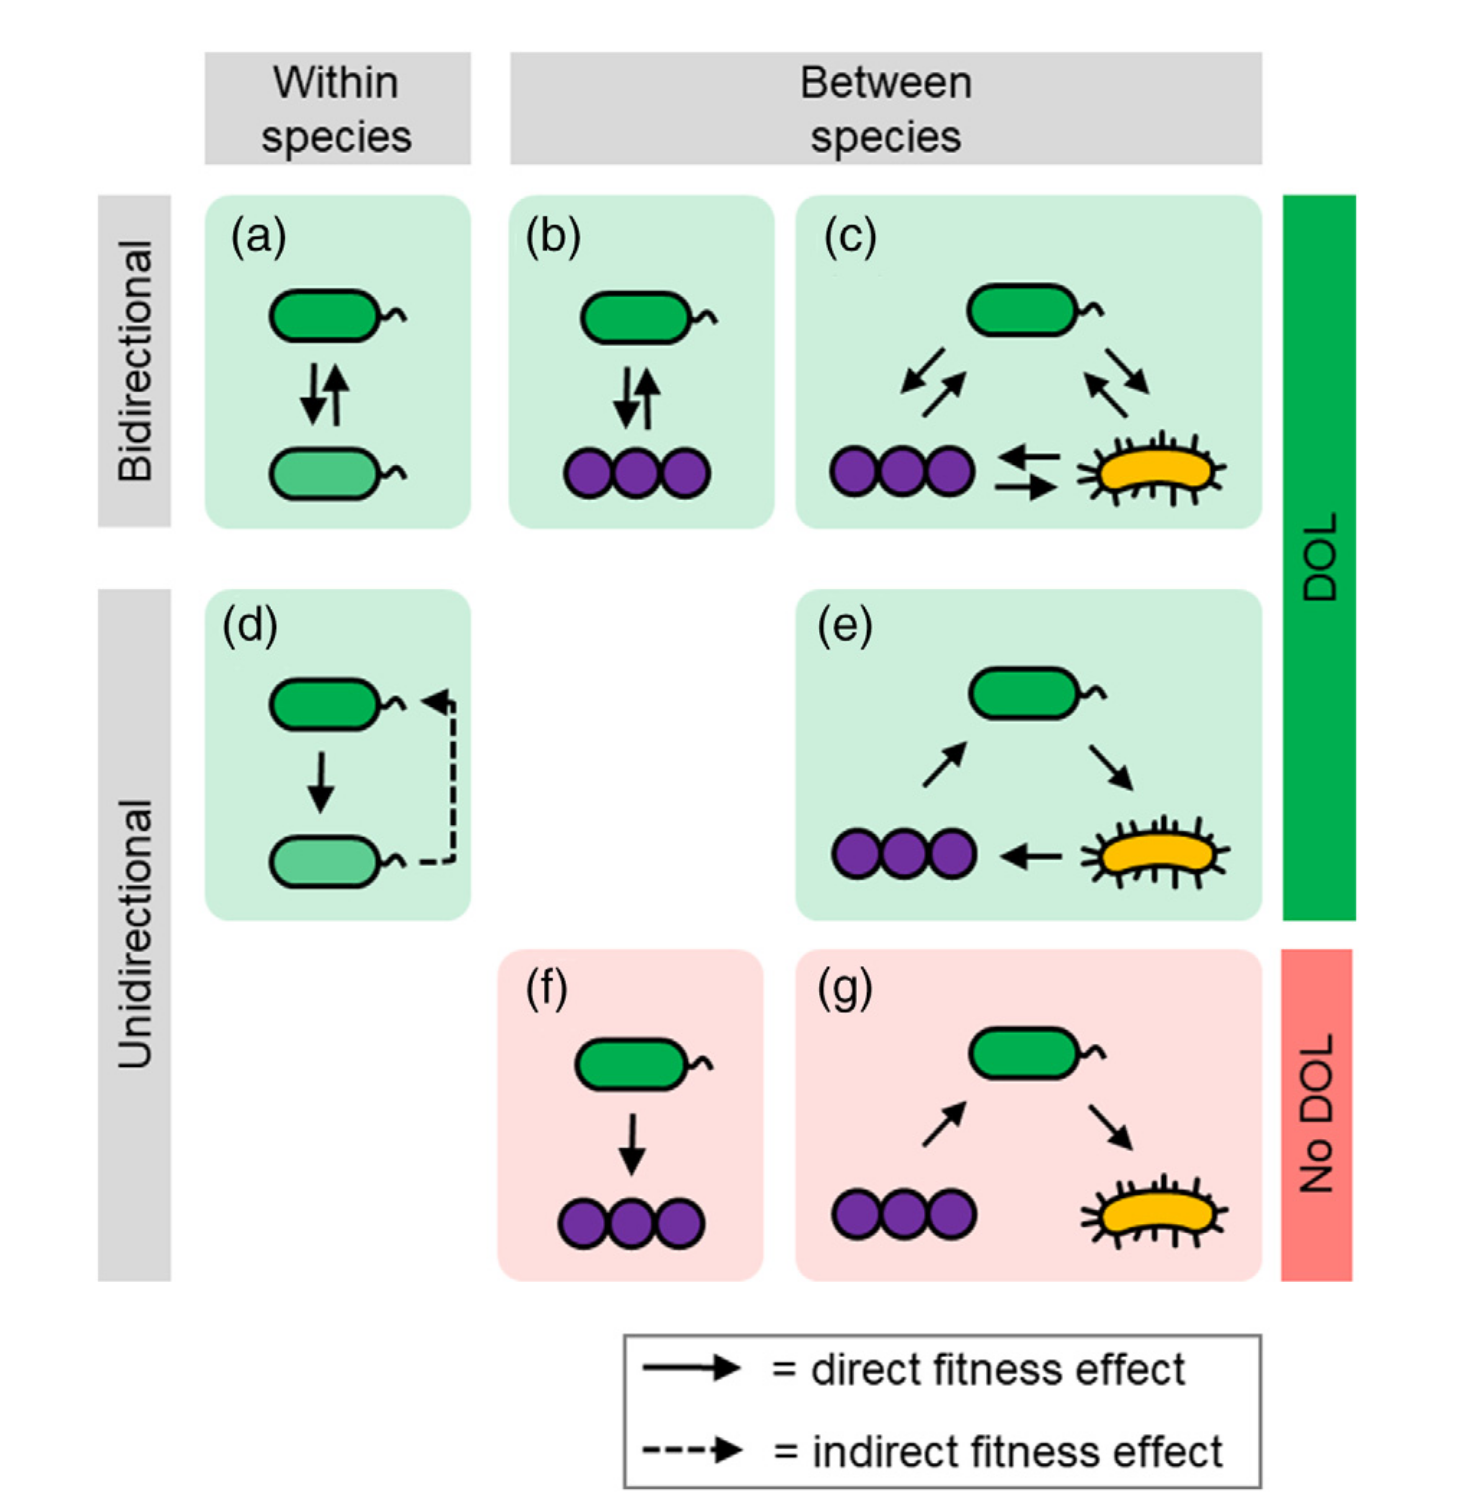
\includegraphics[width=0.6\linewidth,height=\textheight,keepaspectratio]{chapters/../figures/dol_bacteria.png}

}

\caption{\label{fig-microbial-dol}Division of Labor in Microbial
Communities}

\end{figure}%

\emph{Classification of pairwise and three-way interactions as DOL.
Interactions can be uni- or bidirectional as well as occur within one or
between two microbial species. Arrows indicate fitness benefits that are
exchanged between interaction partners that can be direct (straight
line) or indirect (dashed line). For an interaction to classify as DOL,
four main criteria need to be fulfilled, which is only the case in
closed (reciprocal) interactions (green), yet not in open (linear)
interactions (red). (a) Mutually beneficial (reciprocal) interaction
within two conspecific genotypes. (b) Mutually beneficial (reciprocal)
interaction within two heterospecific genotypes. (c) Mutually beneficial
(reciprocal) interaction between three different species. (d)
Unidirectional interaction between two members of the same species. (e)
Unidirectional interaction between three members of three different
species. (f) Unidirectional interaction between two members of two
different species. (g) Unidirectional (linear) interaction chain between
members of three different species.}

\section{Interspecific Division of Labor in Root
Microbiota}\label{interspecific-division-of-labor-in-root-microbiota}

Interspecific DOL has been well-characterized in various ecosystems,
with numerous examples of cross-feeding and mutualistic interactions
documented in the human gut microbiome and soil
communities\textsuperscript{\citeproc{ref-rafieenia2022}{4}}.

The root microbiota represents a particularly well-studied example of
interspecific DOL. Roots of healthy plants host diverse bacteria that
are collectively referred to as the bacterial root microbiota. Unlike
their multicellular eukaryotic hosts that evolved diverse cell-types to
achieve distinct biological functions and promote a division of labour,
unicellular organisms such as bacteria rely on metabolic exchange(s)
with their surrounding biotic environment to establish and maintain
their ecological niches. Recent
reports\textsuperscript{\citeproc{ref-mataigne2021}{5},\citeproc{ref-mataigne2022}{6}},
indicate that metabolic interdependencies and cross-feeding exchanges
are widespread among taxonomically diverse bacteria and likely drive
microbial co-existence within complex bacterial
communities\textsuperscript{\citeproc{ref-estrela2016}{7},\citeproc{ref-adkins-jablonsky2021}{8}}

\section{Intraspecific Division of Labor: An Emerging Research
Area}\label{intraspecific-division-of-labor-an-emerging-research-area}

While interspecific DOL has been extensively studied in various
ecosystems, intraspecific DOL within clonal bacterial populations
remains less explored, despite its potential importance for
understanding population-level adaptation and functional diversity. The
traditional view of biological populations assumed that all individuals
within a clonal population behave identically. However, evidence has
accumulated over decades showing that even genetically identical
organisms can exhibit functional heterogeneity, leading to
population-level benefits through task
specialization\textsuperscript{\citeproc{ref-luxf3pez-paguxe1n2025}{9}}.
While intraspecific division of labor has been well-documented in
multicellular organisms and social insects, its study in bacterial
populations represents a more recent and growing field of research.

\section{Sources of Variation in Intraspecific
DOL}\label{sources-of-variation-in-intraspecific-dol}

Intraspecific DOL emerges through diverse mechanisms that create
functional specialization within populations (produce phenotypic
heterogeneity). These mechanisms can be classified into three main
categories: (1) coordinated specialization, where individuals coordinate
to determine roles through signals, cues, or developmental programs; (2)
random specialization, where each individual adopts a helper phenotype;
and (3) genetic control, where phenotypic differences are determined by
genetic variation between
individuals\textsuperscript{\citeproc{ref-cooper2018}{1},\citeproc{ref-cooper2022}{10}}.

Genetic mecanisme est le plus simple a comprendre : -mutation qui
peuvent entrainer un gain ou une perte de fonction gain-of-function
mutations, where novel capabilities are acquired through genetic
changes, ou modifier l'expression de gènes (loss-of-function mutations,
where genes are inactivated or down-regulated)

-transfert horizontal de gènes ()

Genetic mechanisms represent the most straightforward source of
variation, where heritable mutations lead to gain or loss of
function\textsuperscript{\citeproc{ref-giri2019}{2}}, or horizontal gene
transfer introduces new
capabilities\textsuperscript{\citeproc{ref-cyriaque2024}{11}}. These
changes create stable subpopulations with distinct functional profiles
that persist across generations. The most important causal processes in
this category include: (i) loss-of-function mutations, where genes are
inactivated or down-regulated, creating dependencies on other organisms
that can provide the missing functions; (ii) gain-of-function mutations,
where novel capabilities are acquired through genetic changes; (iii)
horizontal gene transfer, where genetic material is exchanged between
organisms, introducing new metabolic pathways or resistance mechanisms A
particularly striking example involves auxotrophic bacteria - organisms
that have lost genes coding for essential molecules through mutations.
These mutants can survive by relying on helper organisms that provide
the missing
compounds\textsuperscript{\citeproc{ref-pande2014}{12},\citeproc{ref-morris2012}{13}}.
While this creates dependency, it also reduces metabolic costs and
enables specialization within the population, allowing different mutants
to thrive collectively in challenging environments.

However, genetic variation is not the only driver of functional
specialization. Gene expression-based mechanisms involve more complex
regulation of protein synthesis and can create transient or
reversible\textsuperscript{\citeproc{ref-dekkers1998}{14}} functional
specialization that may eventually become genetically encoded. Random
fluctuations in gene expression due to the inherent
noise\textsuperscript{\citeproc{ref-raj2008}{15}--\citeproc{ref-keren2015}{17}}
in biological systems can lead to phenotypic heterogeneity even among
genetically identical cells. This noise-driven variation can create
functional diversity that benefits the population as a whole. Building
upon this concept, the novel theory of noise-averaging cooperation
(NAC)\textsuperscript{\citeproc{ref-lopez2022}{18}} explains how
stochastic metabolic noise can drive the emergence of cross-feeding
interactions and metabolic interdependencies. Due to their small size,
bacteria experience substantial noise in metabolic regulation, which
limits individual growth rates. To compensate, related bacteria can
share metabolites to `average out' this noise and improve collective
growth. This metabolite sharing, or `leakage', can then facilitate the
evolution of metabolic interdependencies and even drive speciation
through gene deletions, as predicted by the Black Queen
Hypothesis\textsuperscript{\citeproc{ref-morris2012}{13}}. The Black
Queen Hypothesis, proposed by Morris and colleagues, suggests that in
environments where certain functions are costly to maintain but
beneficial to the community, some organisms may lose these functions
(becoming ``leaky'') while others retain them, creating metabolic
interdependencies. NAC thus provides a mechanistic link between
stochastic gene expression noise and the emergence of genetic
specialization within populations, bridging the gap between phenotypic
and genetic mechanisms of variation.

Environmental regulation further complicates this picture, as
differential gene expression driven by microenvironmental cues and
cellular perception of local
conditions\textsuperscript{\citeproc{ref-korshoj2024}{19}} can create
spatial or temporal patterns of functional specialization within
populations. These environmentally-induced variations can become
stabilized through genetic changes if they confer consistent fitness
benefits, illustrating how phenotypic plasticity can drive evolutionary
innovation.

These mechanisms often interact and overlap, making it challenging to
distinguish between them. Factors such as growth/defense trade-offs,
physiological state, growth stage, and even cell lysis can contribute to
functional heterogeneity within populations. Importantly, phenotypic
variation can provide the substrate for genetic evolution - stochastic
gene expression patterns that confer fitness benefits may become
stabilized through genetic changes over time. This evolutionary
perspective highlights how the division of labor within populations can
emerge through a complex interplay of immediate phenotypic responses and
long-term genetic adaptation. The resolution of measurement techniques
and the capacity to detect variation between cells (now possible with
single-cell technologies) are crucial for understanding these complex
interactions and their evolutionary implications.

The root environment presents unique challenges and opportunities for
bacterial colonization. The rhizosphere, the soil region directly
influenced by root exudates, represents a nutrient-rich but competitive
environment where bacteria must balance resource acquisition with
defense against competitors. This complex ecosystem provides an ideal
setting for studying how bacterial populations adapt through functional
specialization and metabolic cooperation.

• Enzymes spécifiques de voies métaboliques

• Facteurs de virulence ou de stress

• Gènes liés au quorum sensing (\emph{luxR, lasI}\ldots)

• Transporteurs de fer (sidérophores)

Comme tu analyses \textbf{Pseudomonas brassicacearum en stress de fer},
il serait intéressant de vérifier :

• L'expression des gènes de \textbf{sidérophores} (\emph{pch},
\emph{ent}, \emph{pyoverdine})

• La régulation de \textbf{facteurs sigma} (\emph{rpoS}, \emph{rpoN})

• La présence de \textbf{différenciation métabolique} entre
sous-populations

(a specialized role that benefits the group, such as producing public
goods or performing specific metabolic functions) with a certain
probability independently

, or horizontal gene transfer introduces new
capabilities\textsuperscript{\citeproc{ref-cyriaque2024}{11}} \#\# Model
Organism: Pseudomonas brassicacearum R401

Successful establishment of bacteria at roots is driven by multiple
independent biological processes involved in both host-microbe (i.e.,
signal recognition, chemotaxis, surface attachment, biofilm formation,
virulence factors) and microbe-microbe interactions (i.e., production of
antimicrobials or public goods) (Knights et al.~2021). Therefore, we
postulate that the simultaneous activation of these diverse processes is
costly and that cooperation between genetically identical strains is key
for promoting bacterial pervasiveness at roots. Consistent with this
hypothesis, we recently demonstrated that the robust root coloniser
Pseudomonas brassicacearum R401 (hereafter referred to as PsR401)
deploys multiple independent strategies that co-function to promote
colonisation and persistence at roots (Getzke et al., 2023). Notably, we
identified two independent processes involved in microbe-microbe
competition -- namely the production of an antimicrobial and of a
molecule scavenging the micronutrient iron -- that act additively to
promote strain competitiveness at roots (Getzke et al., 2023). We
identified a third bacterial locus in PsR401 involved in the production
of a phytotoxin that promotes both pathogenicity and root colonisation
in mono-association experiments with A. thaliana (unpublished, see
below). Our work provides proof-of-concept data illustrating that PsR401
deploys diverse exo-metabolites during root microbiota establishment
that have versatile functions in host-microbe and microbe-microbe
interactions. Together with earlier work (Gu et al.~2020, Harbort et al
2020), it also delineates iron as a major micronutrient modulating
strain competitiveness and proliferation at roots. Given that the public
good iron becomes rate-limiting in the root compartment and that
production of the above-mentioned processes are all modulated by iron
availability (Lim et al., 2012; Palma et al., 2003, Mo et al.~1991), we
anticipate that division of labour between bacterial intra-populations
is bolstered under iron limiting conditions such as those found in the
root habitat.

Our study focuses on \emph{Pseudomonas brassicacearum} R401 (PsR401), a
robust root colonizer of \emph{Arabidopsis thaliana} that can act as an
opportunistic pathogen. This strain represents an excellent model for
studying intraspecific DOL due to its complex colonization strategies
and environmental adaptability.

\subsection{Colonization Strategies}\label{colonization-strategies}

PsR401 deploys multiple independent strategies for root colonization and
persistence:

\begin{itemize}
\tightlist
\item
  \textbf{Antimicrobial production}: Suppresses competitors in the
  rhizosphere
\item
  \textbf{Siderophore production}: Enhances iron acquisition and
  competitiveness by sequestering iron
\item
  \textbf{Phytotoxin production}: Promotes both pathogenicity and root
  colonization
\end{itemize}

\subsection{Iron as a Key Limiting
Factor}\label{iron-as-a-key-limiting-factor}

These processes are all modulated by iron availability, which becomes
rate-limiting in the root compartment. Iron acts as a ``public good'' in
the rhizosphere - all bacteria require it, but it is scarce in the
environment. Given that the production of antimicrobials, siderophores,
and phytotoxines is energetically costly and iron-dependent, we
hypothesize that division of labor between bacterial intra-populations
is bolstered under iron-limiting conditions.

\section{Single-Cell Technologies: Unveiling Cellular
Heterogeneity}\label{single-cell-technologies-unveiling-cellular-heterogeneity}

Single-cell technologies have revolutionized our understanding of
cellular diversity in eukaryotic systems. Methods such as scRNA-seq,
scATAC-seq, scMetabolomics, and spatial omics have provided
unprecedented insights into cellular heterogeneity and functional
specialization. These new technologies allow us to access within-species
diversity and study the possible metabolic specialization between cells.
Single-cell omics have been developed for this purpose in human health
and are now applied to microbial systems. However, analyzing such
datasets still requires custom pipelines to respond to the specificity
of bacterial biology and technical challenges.

\subsection{Technical Challenges in Bacterial Single-Cell
RNA-seq}\label{technical-challenges-in-bacterial-single-cell-rna-seq}

However, applying these technologies to bacterial systems presents
unique challenges:

\begin{itemize}
\tightlist
\item
  \textbf{Lack of poly-A tails}: Bacterial mRNAs lack poly-A tails,
  requiring alternative capture methods
\item
  \textbf{High rRNA content}: rRNA constitutes up to 95\% of bacterial
  RNA, necessitating effective depletion strategies
\item
  \textbf{Low RNA content}: Bacterial cells contain much less RNA than
  mammalian cells
\item
  \textbf{Cell wall complexity}: Diverse cell wall structures complicate
  RNA extraction
\item
  \textbf{Operon structure}: Bacterial operons require specific
  approaches for complete capture
\item
  \textbf{Small RNA detection}: Regulatory sRNAs are challenging to
  detect due to their short length
\end{itemize}

\subsection{Methodological Approaches}\label{methodological-approaches}

Several approaches have been developed to address these challenges:

\begin{itemize}
\tightlist
\item
  \textbf{Plate-based methods}: High sensitivity but low throughput
  (hundreds of cells)
\item
  \textbf{Split-pool barcoding}: High throughput with moderate
  sensitivity (microSPLiT)
\item
  \textbf{Droplet-based methods}: Balance between throughput and
  sensitivity
\end{itemize}

\section{Research Objectives and Experimental
Approach}\label{research-objectives-and-experimental-approach}

\subsection{Primary Research Question}\label{primary-research-question}

The goal of this internship is to explore scRNA-seq (single-cell
RNA-seq) datasets of \emph{Pseudomonas brassicacearum}, a root
colonizer. The student will analyze sample datasets from various
nutritional conditions to determine if DOL can be detected within this
species as a strategy for efficient root colonization.

The central question of this study is: \textbf{Is there functional
specialization (DOL) within clonal populations of PsR401?}

This question addresses two main biological hypotheses:

\begin{enumerate}
\def\labelenumi{\arabic{enumi}.}
\tightlist
\item
  \textbf{Noisy regulation hypothesis}: Gene expression varies
  stochastically between identical cells
\item
  \textbf{Specialized cells hypothesis}: Certain cells become
  functionally specialized under specific conditions
\end{enumerate}

\subsection{Experimental Design}\label{experimental-design}

We employ the microSPLiT
technology\textsuperscript{\citeproc{ref-kuchina2021}{20}}, a
high-throughput single-cell RNA sequencing method for bacteria developed
from SPLiT-seq for eukaryotic cells. This method allows for the analysis
of transcriptomic heterogeneity within bacterial populations at
single-cell resolution, providing insights into gene expression patterns
and cellular diversity that would be masked in bulk RNA-seq approaches.

The experimental setup includes: - \textbf{Controlled conditions}:
Iron-limiting and glucose-limiting environments - \textbf{Time course
analysis}: During exponential growth phase - \textbf{Multiple
replicates}: Biological and technical replicates for robust analysis -
\textbf{High-throughput sequencing}: Targeting \textasciitilde3,000
cells with \textasciitilde1.5 billion reads

This approach will provide mechanistic insights into whether and how a
robust bacterial root colonizer can partition tasks within
intra-populations to achieve greater functional diversity, minimize
energetic costs, and adapt to environmental constraints.

The ANR DivIDE project seeks to understand the mechanisms of division of
labor in bacterial populations, with WP2 focusing on transcriptional
variation supporting intraspecific DOL. This internship represents a
first approach to exploring these complex interactions at the
single-cell level.

\bookmarksetup{startatroot}

\chapter{Materials and Methods}\label{sec-materials-and-methods}

\section{Bacterial culture}\label{bacterial-culture}

\begin{figure}

\centering{

\includegraphics[width=4in,height=3in]{chapters/02-Materials-and-methods_files/figure-latex/mermaid-figure-1.png}

}

\caption{\label{fig-experimental-design}Experimental design for
bacterial culture}

\end{figure}%

\emph{The workflow illustrates the progression from initial culture of
P. brassicacearum R401 on petri dishes to liquid culture in two
different media: M9 (low glucose and iron) and M9F (high glucose and
iron). Each medium condition was replicated three times (Rep A, B, C)
and growth was monitored at three timepoints (T1, T2, T3) by optical
density measurements. This design resulted in 18 total experimental
conditions (2 media × 3 biological replicates × 3 timepoints) for
subsequent single-cell RNA-seq analysis.}

An isogenic\footnote{An isogenic population refers to a group of
  organisms that are genetically identical, derived from a single
  ancestral cell or clone.} population of \emph{P. brassicacearum} R401
was initially cultured on petri dishes and then transferred to different
liquid media to investigate the effects of nutrient availability on
bacterial growth and gene expression
(Figure~\ref{fig-experimental-design}).

Two distinct culture conditions were applied to the bacteria: M9 medium
containing low glucose and low iron concentrations, and M9F medium
containing high glucose and high iron concentrations (see
Table~\ref{tbl-media} for detailed concentrations). Each condition was
replicated three times to ensure statistical robustness of the
experimental results. The bacterial growth was monitored by measuring
optical density (OD) at regular intervals. The growth curves obtained
from these measurements are presented (Figure~\ref{fig-growth-curves})
and (Table~\ref{tbl-growth-curves}). This experimental design resulted
in a total of 18 conditions: 2 media types × 3 biological replicates × 3
time points, providing comprehensive coverage of the growth dynamics
under different nutrient conditions.

\begin{figure}

\centering{

\pandocbounded{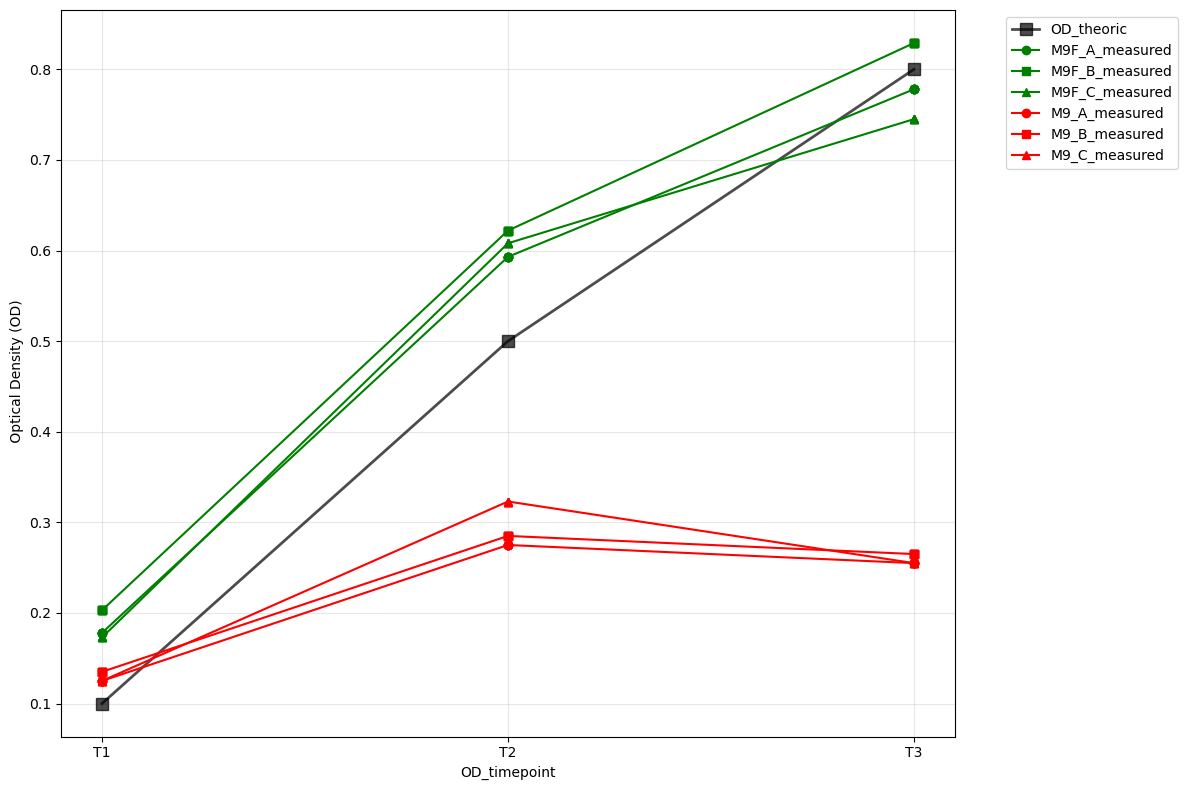
\includegraphics[keepaspectratio]{chapters/../figures/growth_curves.png}}

}

\caption{\label{fig-growth-curves}Bacterial growth dynamics of \emph{P.
brassicacearum} R401 populations measured by optical density (OD600)
cultured under two different nutrient conditions: M9 (low glucose/iron)
and M9F (high glucose/iron).}

\end{figure}%

\emph{Measurements were taken at three timepoints (T1, T2, T3) for three
biological replicates (Rep A, B, C).}

The growth curves reveal distinct patterns between the two culture
conditions. Bacteria grown in M9F medium (high glucose and iron)
exhibited significantly higher growth rates and reached higher optical
densities (OD 0.17-0.21 at T1, 0.59-0.63 at T2, 0.74-0.83 at T3)
compared to M9 medium (low glucose and iron) which showed limited growth
(OD 0.13 at T1, 0.28-0.33 at T2, 0.26 at T3). While M9F cultures showed
continued growth from T2 to T3, the growth rate slowed down during this
period, indicating the beginning of transition towards stationary phase.
The M9 cultures appeared to reach a growth plateau by T3, while M9F
cultures maintained higher densities despite the growth deceleration,
suggesting nutrient limitation in the M9 condition. Biological
replicates showed excellent reproducibility validating the experimental
design.

Cells were collected at each timepoint (T1, T2, T3) from all biological
replicates for subsequent single-cell RNA-seq analysis using the
Microbial split-pool ligation transcriptomics (microSPLiT)
protocol\textsuperscript{\citeproc{ref-kuchina2021}{20},\citeproc{ref-gaisser2024}{21}}.

\section{microSPLiT protocol}\label{microsplit-protocol}

MicroSPLiT\textsuperscript{\citeproc{ref-kuchina2021}{20},\citeproc{ref-gaisser2024}{21}}
is a high-throughput single-cell RNA sequencing method for bacteria,
capable of profiling transcriptional states in hundreds of thousands of
cells per experiment without the need for specialized
equipment\textsuperscript{\citeproc{ref-gaisser2024}{21},\citeproc{ref-nishimura2025}{22}}.
Unlike other single-cell RNA-seq approaches that require physical
isolation of individual cells (e.g., plate-based or droplet-based
methods), microSPLiT uses a split-pool barcoding strategy to uniquely
label transcripts within each cell. (see
Figure~\ref{fig-nishimura_review} for an overview of single-cell RNA-seq
methods in bacteria)

\begin{tcolorbox}[enhanced jigsaw, colbacktitle=quarto-callout-tip-color!10!white, bottomtitle=1mm, coltitle=black, colframe=quarto-callout-tip-color-frame, left=2mm, bottomrule=.15mm, rightrule=.15mm, opacityback=0, toptitle=1mm, colback=white, title=\textcolor{quarto-callout-tip-color}{\faLightbulb}\hspace{0.5em}{Information}, arc=.35mm, toprule=.15mm, breakable, leftrule=.75mm, opacitybacktitle=0.6, titlerule=0mm]

The microSPLiT strategy will not be described in detail here; for more
information, see Gaisser
protocol.\textsuperscript{\citeproc{ref-gaisser2024}{21}}. Only the key
steps necessary for a general understanding of the method are presented
below.

\end{tcolorbox}

\begin{figure}

\centering{

\pandocbounded{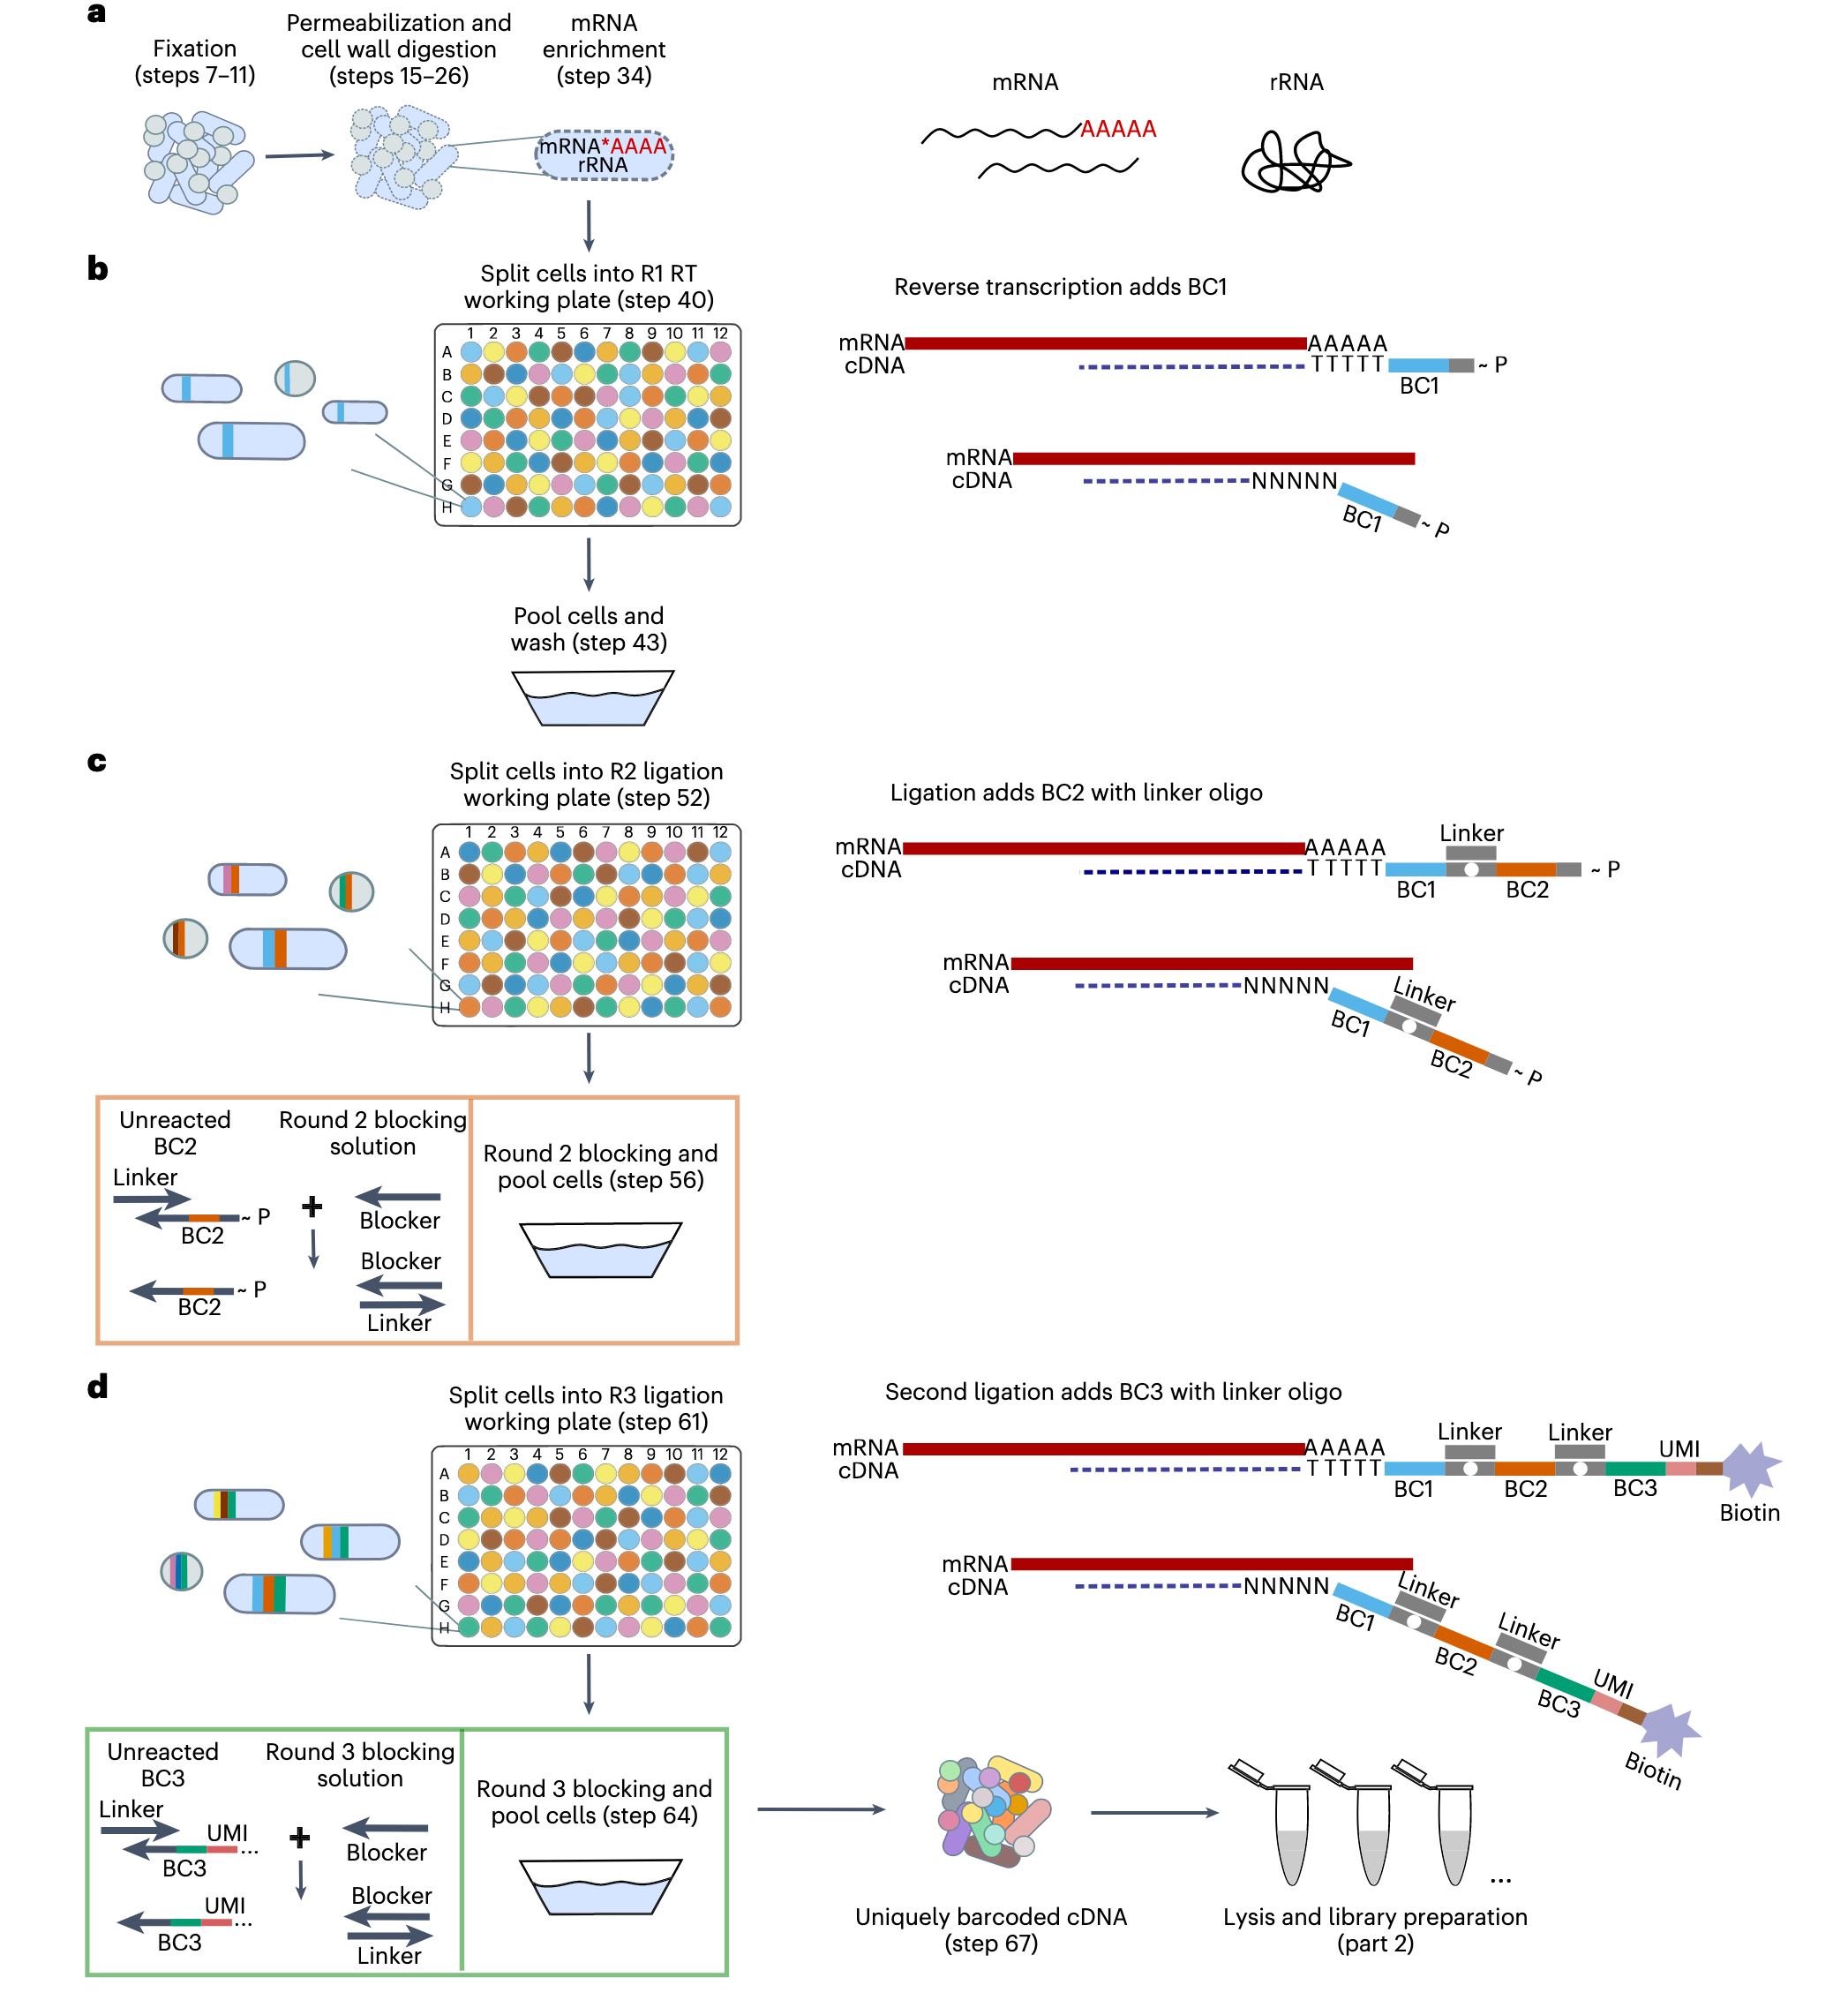
\includegraphics[keepaspectratio]{chapters/../figures/protocol.png}}

}

\caption{\label{fig-protocol}MicroSPLiT in-cell cDNA barcoding scheme.}

\end{figure}%

\emph{a, Bacterial cells are fixed overnight and permeabilized before
the mRNA is preferentially polyadenylated. After mRNA enrichment, cells
may contain both polyadenylated and non-polyadenylated mRNA. b, Cells
are distributed into the first barcoding plate, and the mRNA is reverse
transcribed by using a mixture of poly-dT and random hexamer primers
carrying a barcode (barcode 1, BC1) and a 5' phosphate for future
ligation at their 5' end. After the barcoding reaction, cells are pooled
together and split again into the second barcoded plate. c, Ligation
adds a 5' phosphorylated barcode 2 (BC2) to BC1 with a linker strand. A
blocking solution is then added to each of the wells of the second
plate, preventing any unreacted BC2 from future ligation. Cells are
pooled and split into the third and final barcoded plate. d, A second
ligation step adds barcode 3 (BC3) with another linker strand. BC3 also
contains a 5' biotin, a primer binding site and a unique molecular
identifier (UMI). A blocking solution for the R3 linker is added to each
of the wells in the plate before the final pooling of cells. This
results in uniquely barcoded cells that can be distributed in aliquots
into sub-libraries and stored until future use or used immediately for
library preparation. (R1, round 1; R2, round 2; R3, round
3).\textsuperscript{\citeproc{ref-gaisser2024}{21}}}

\subsection{Fixation and
permeabilization}\label{fixation-and-permeabilization}

The first step is fixation of the bacterial suspension with formaldehyde
Figure~\ref{fig-protocol} immediately after sampling the 18 conditions
Figure~\ref{fig-experimental-design}. This preserves the transcriptomic
state and cross-links RNA to proteins, preventing leakage of each cell's
transcriptome. Next, cells are permeabilized using mild detergent and
lysozyme, allowing enzymes and oligonucleotides to access intracellular
RNA for barcoding.

\begin{tcolorbox}[enhanced jigsaw, colbacktitle=quarto-callout-note-color!10!white, bottomtitle=1mm, coltitle=black, colframe=quarto-callout-note-color-frame, left=2mm, bottomrule=.15mm, rightrule=.15mm, opacityback=0, toptitle=1mm, colback=white, title=\textcolor{quarto-callout-note-color}{\faInfo}\hspace{0.5em}{Note}, arc=.35mm, toprule=.15mm, breakable, leftrule=.75mm, opacitybacktitle=0.6, titlerule=0mm]

Adequate permeabilization is essential for efficient barcoding, but
over-permeabilization can compromise cell integrity. For successful
single-cell resolution, cells must remain intact after permeabilization
to allow multiple split-pool steps and retain cross-linked RNA.
Figure~\ref{fig-protocol}

\end{tcolorbox}

\subsection{mRNA enrichment}\label{mrna-enrichment}

After permeabilization, the transcripts in the fixed and permeabilized
cells undergo in situ polyadenylation with the addition of a poly(A)
polymerase (PAP) and ATP. This step enriches for mRNA in the total
barcoded RNA pool because, under these conditions, PAP preferentially
polyadenylates mRNA as opposed to ribosomique RNA (rRNA)
Figure~\ref{fig-protocol}.

\subsection{Barcoding}\label{barcoding}

\begin{tcolorbox}[enhanced jigsaw, colbacktitle=quarto-callout-tip-color!10!white, bottomtitle=1mm, coltitle=black, colframe=quarto-callout-tip-color-frame, left=2mm, bottomrule=.15mm, rightrule=.15mm, opacityback=0, toptitle=1mm, colback=white, title=\textcolor{quarto-callout-tip-color}{\faLightbulb}\hspace{0.5em}{Tip}, arc=.35mm, toprule=.15mm, breakable, leftrule=.75mm, opacitybacktitle=0.6, titlerule=0mm]

\textbf{The protocol utilizes several rounds of split-pool barcoding
where cells are distributed into 96-well plates, barcoded, pooled, and
redistributed for subsequent rounds, creating unique barcode
combinations that identify individual cells.}

\end{tcolorbox}

\subsubsection{Barcoding round 1 (R1) to identify the condition and the
technical
replicate}\label{barcoding-round-1-r1-to-identify-the-condition-and-the-technical-replicate}

Each of the 18 samples is split into 5 technical replicates for
barcoding, resulting in 90 subsamples. These technical replicates are
then distributed into individual wells of a 96-well plate (6 wells not
used), with each well containing uniquely barcoded primers
Figure~\ref{fig-protocol}. In each well, mRNA is reverse transcribed
into cDNA using a mix of barcoded poly(T) and random hexamer primers.
The primers used in each well contain either a dT15 sequence to capture
polyadenylated mRNA or six random nucleotides to bind any RNA, followed
by a universal sequence for subsequent ligation steps. By assigning each
technical replicate to a specific well, all cells in the same well
receive the same unique barcode during reverse transcription. This
allows each technical replicate and condition to be identified later
based on the first barcode.

\subsubsection{Barcoding rounds 2 (R2) and 3 (R3) for unique cell and
transcript
identification}\label{barcoding-rounds-2-r2-and-3-r3-for-unique-cell-and-transcript-identification}

Cells are then pooled, washed and randomly redistributed into a new
96-well plate (round 2 (R2) ligation working plate) containing a second
set of well-specific barcodes, which are appended to the first barcode
on the cDNA through an in-cell ligation reaction
Figure~\ref{fig-protocol}. Due to the random redistribution of cells,
each well of the second-round plate is likely to contain a mix of cells
with different first-round barcodes, resulting in highly diverse barcode
combinations. The ligation reaction is carried out by the T4 DNA ligase,
which requires double-stranded DNA. Therefore, in the second barcoding
plate, each barcode is first hybridized to a short linker
oligonucleotide whose overhang is complementary to the universal
sequence at the 5' end of the RT barcodes. Figure~\ref{fig-protocol}.

\begin{tcolorbox}[enhanced jigsaw, colbacktitle=quarto-callout-note-color!10!white, bottomtitle=1mm, coltitle=black, colframe=quarto-callout-note-color-frame, left=2mm, bottomrule=.15mm, rightrule=.15mm, opacityback=0, toptitle=1mm, colback=white, title=\textcolor{quarto-callout-note-color}{\faInfo}\hspace{0.5em}{Note}, arc=.35mm, toprule=.15mm, breakable, leftrule=.75mm, opacitybacktitle=0.6, titlerule=0mm]

After the ligation step, some barcodes may remain unreacted in the
solution. To prevent these free barcodes from attaching non-specifically
to DNA from other cells during pooling, a blocker strand is added. This
blocker has a longer complementary region to the linker, allowing it to
displace any unreacted barcodes from the linker and thus ensures that
only correctly ligated barcodes remain attached to the cDNA.
Figure~\ref{fig-protocol}

\end{tcolorbox}

Cells are then pooled again, and a split-ligation-pool cycle is repeated
for the second time. Cells are randomly distributed into a third 96-well
plate (round 3 (R3) ligation working plate), which is loaded with
barcoded oligonucleotides containing the third cell barcode annealed
with a linker, a 10-base Unique Molecular Identifier (UMI), a universal
PCR handle and a 5' biotin\footnote{Biotin is a small vitamin molecule
  that binds with extremely high affinity to streptavidin. This
  biotin-streptavidin interaction is used for the selective capture and
  purification of biotinylated cDNA molecules on streptavidin-coated
  beads during the library preparation process.} molecule. The ligation
reaction is stopped by adding a second blocker strand and EDTA.

\begin{tcolorbox}[enhanced jigsaw, colbacktitle=quarto-callout-warning-color!10!white, bottomtitle=1mm, coltitle=black, colframe=quarto-callout-warning-color-frame, left=2mm, bottomrule=.15mm, rightrule=.15mm, opacityback=0, toptitle=1mm, colback=white, title=\textcolor{quarto-callout-warning-color}{\faExclamationTriangle}\hspace{0.5em}{Warning}, arc=.35mm, toprule=.15mm, breakable, leftrule=.75mm, opacitybacktitle=0.6, titlerule=0mm]

In our experiment, only 95 out of the 96 wells of the R3 plate are used
to minimize potential bias in cell distribution. This setup allows for
90 × 96 × 95 = \textbf{820,800 possible barcode combinations}, enabling
the identification of up to 820,800 individual cells.

\end{tcolorbox}

\subsection{Sub-library and sequencing
preparation}\label{sub-library-and-sequencing-preparation}

The pooled cells are washed, counted, and divided into multiple
sub-libraries. Only sub-libraries containing approximately 3,000 cells
were selected for sequencing, in order to maximize sequencing depth per
cell and minimize barcode collision rates which is the probability that
two cells receive the same barcode combination.

After lysis and cDNA purification on streptavidin beads
(Figure~\ref{fig-protocol-p2}), a second reverse transcription is
performed to improve cDNA yield, during which a template switch oligo
(TSO) is added to introduce a 3' adapter. The resulting cDNA is then
amplified by PCR. Following amplification, a size selection step removes
short byproducts such as adapter or barcode dimers, ensuring that only
high-quality cDNA fragments are retained for sequencing.

To optimize sequencing depth, the final library was split into four
sub-libraries, each receiving a distinct index during adapter ligation:
BC\_0076 (CAGATC), BC\_0077 (ACTTGA), BC\_0078 (TAGCTT), and BC\_0079
(GGCTAC). These indexes were used solely to improve sequencing quality
and balance on the NovaSeq platform, without introducing any
experimental or technical variation between sub-libraries.

\subsection{Sequencing and demultiplexing
sub-libraries}\label{sequencing-and-demultiplexing-sub-libraries}

Sequencing was performed on a NovaSeq\textsuperscript{TM} X plus
instrument at GenoBIRD platform in paired-end mode. The library pool was
loaded onto all lanes of the flowcell at a final concentration of 200 pM
with 20\% PhiX\footnote{PhiX is a control library containing a known
  viral genome sequence that is spiked into sequencing runs to monitor
  sequencing quality, calibrate base calling, and provide a reference
  for quality control metrics. It helps ensure accurate sequencing
  performance and data quality assessment.}. The sequencing program
consisted of 241 cycles for Read 1, 6 cycles for Index i7 and 91 cycles
for Read 2. The sequencing facility performed demultiplexing of
sub-libraries, resulting in eight FASTQ files (R1 and R2 for each
index). R1 files contain the cDNA sequences, while R2 files contain the
cell barcodes (from the three split-pool rounds) and unique molecular
identifiers (UMIs).

\begin{itemize}
\tightlist
\item
  For each index, two paired-end FASTQ files were generated :

  \begin{itemize}
  \tightlist
  \item
    \textbf{R1} contains the cDNA sequence of interest (transcriptome).
  \item
    \textbf{R2} contains the cell barcodes and unique molecular
    identifiers (UMIs).
  \end{itemize}
\end{itemize}

\section{Pipeline for microSPLiT data
processing}\label{pipeline-for-microsplit-data-processing}

\begin{figure}

\centering{

\pandocbounded{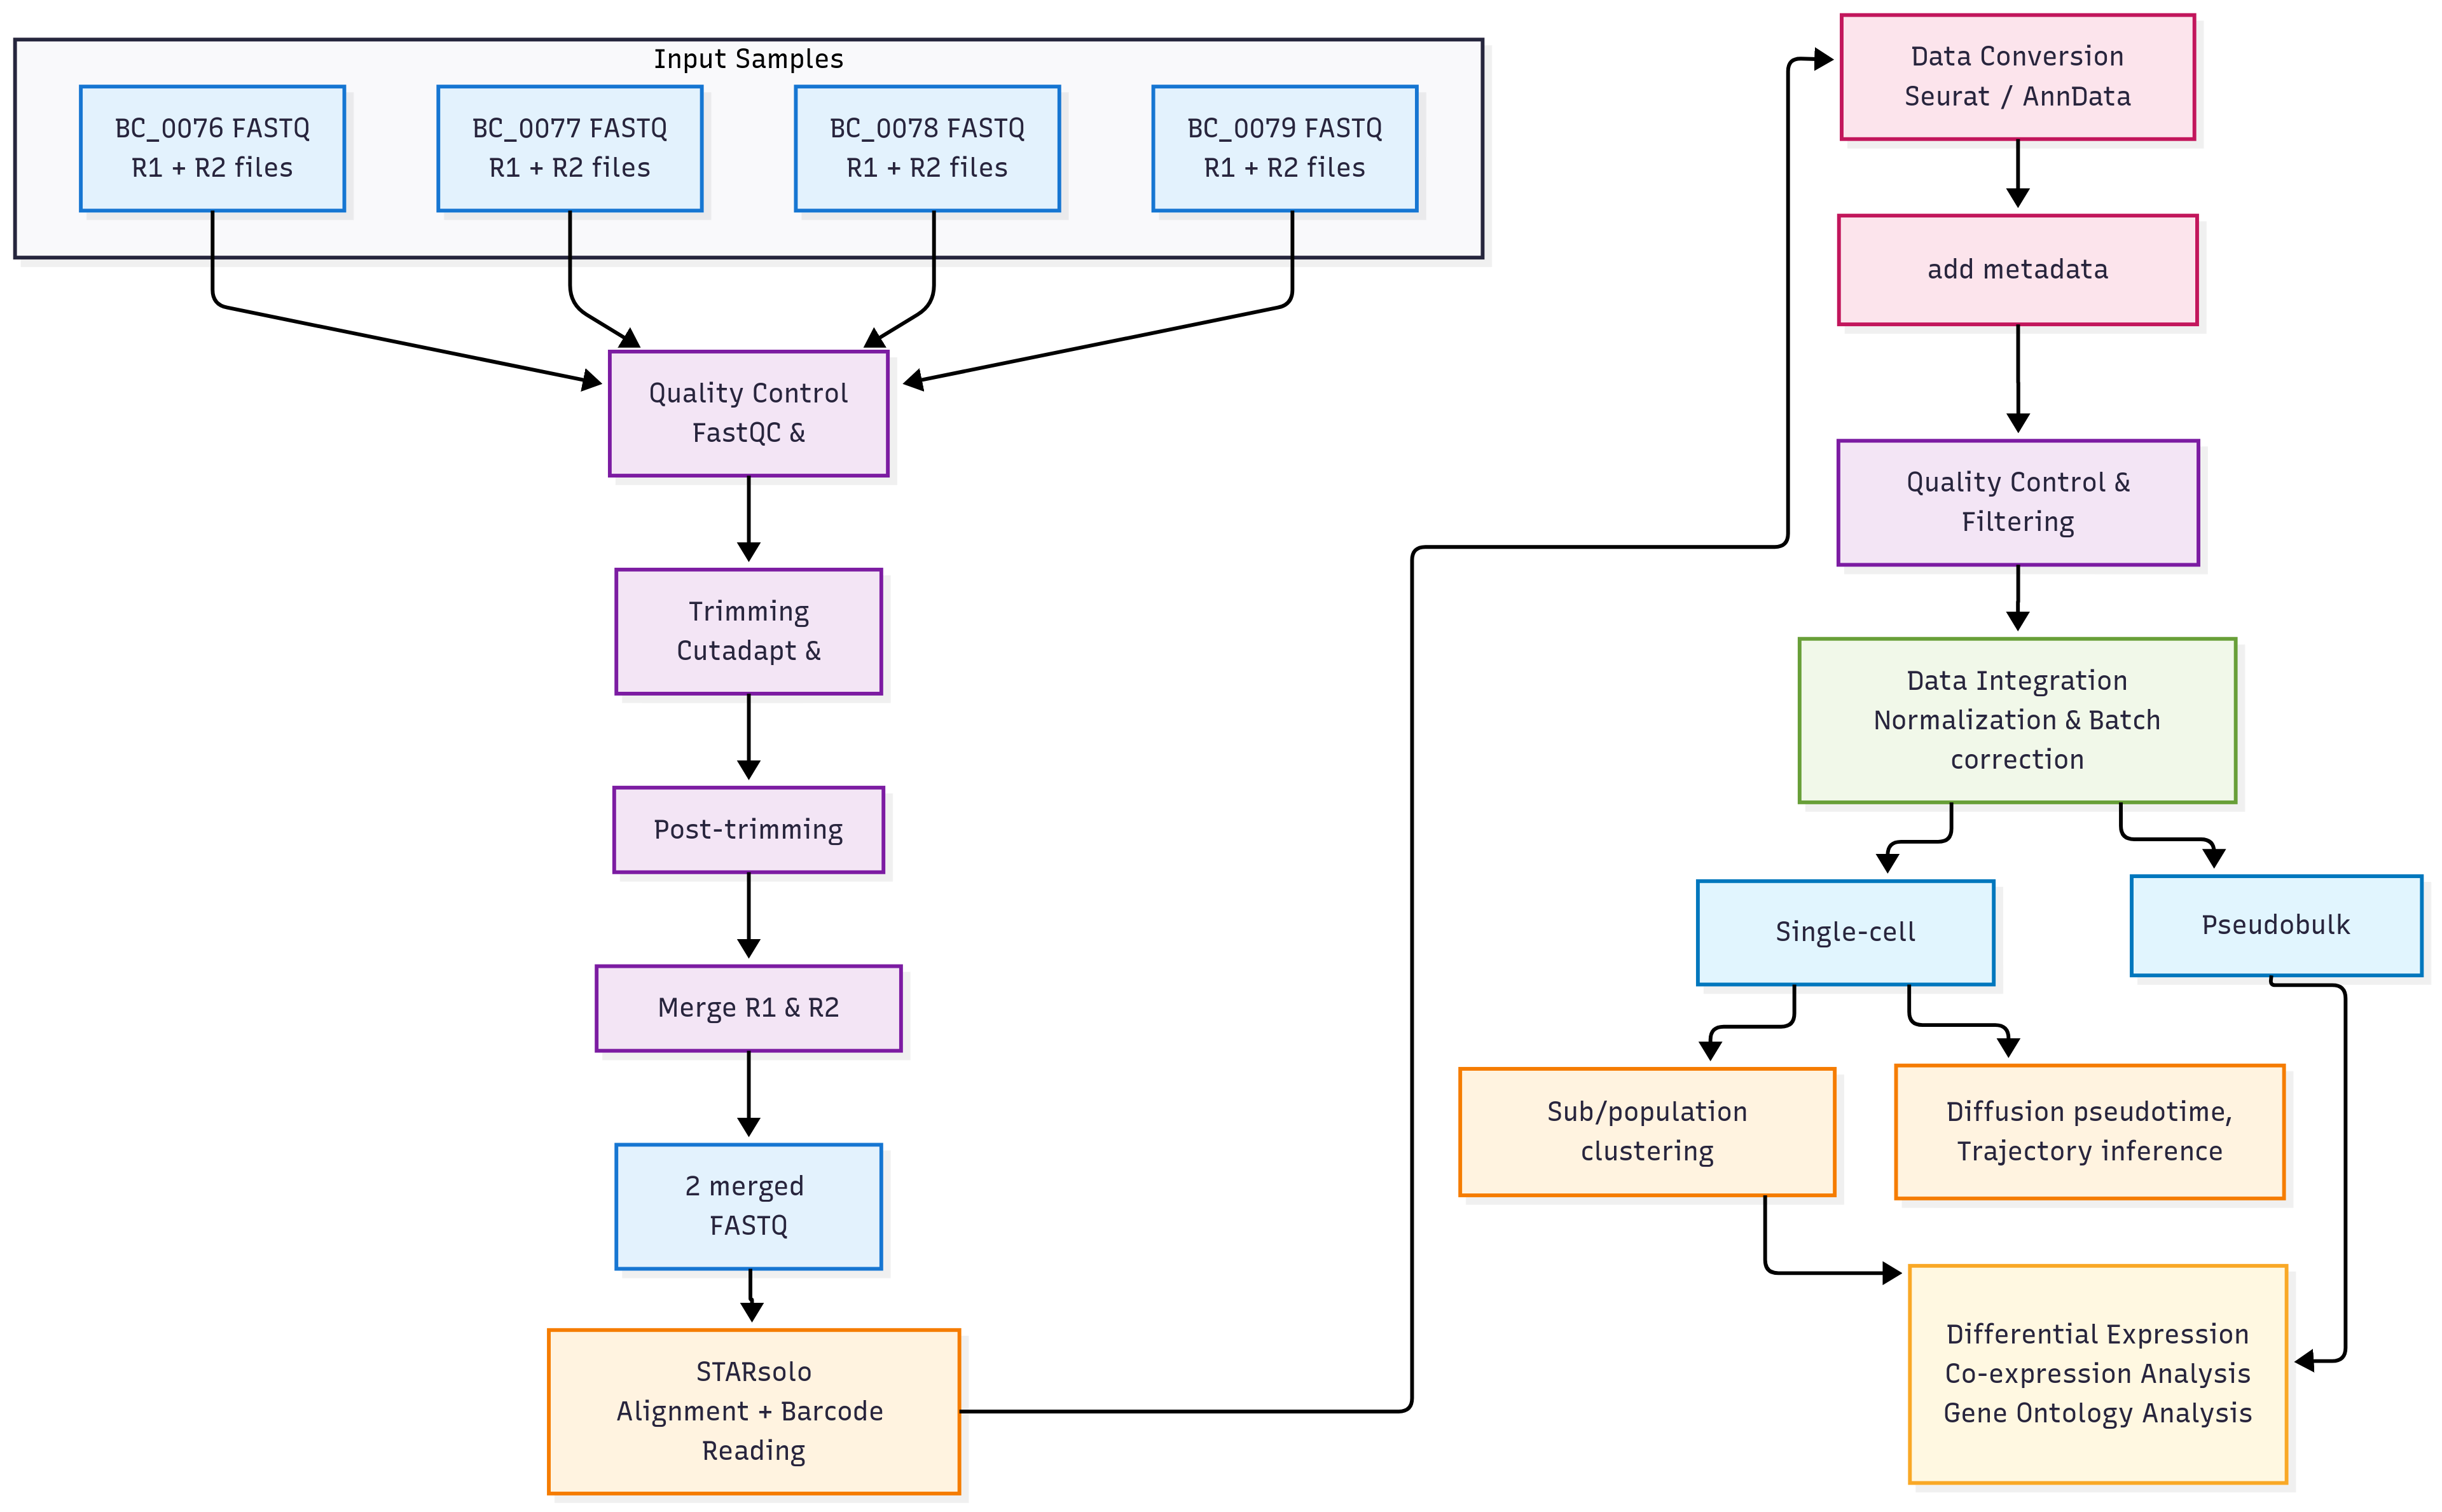
\includegraphics[keepaspectratio]{chapters/../figures/pipeline.png}}

}

\caption{\label{fig-pipeline}Comprehensive pipeline for microSPLiT
single-cell RNA-seq data processing.}

\end{figure}%

\emph{The workflow encompasses the complete analytical process from raw
sequencing data to biological interpretation, including quality control
and preprocessing of FASTQ files, alignment and quantification using
STARsolo, data structuring with metadata assignment, quality filtering
and integration, single-cell and pseudobulk analysis approaches,
population characterization through clustering and trajectory inference,
and downstream expression analysis including differential expression,
co-expression networks, and gene ontology enrichment.
Figure~\ref{fig-pipeline}}

\subsection{Preprocessing of the sequencing
data}\label{preprocessing-of-the-sequencing-data}

All quality control, trimming, alignment, barcode reading and generation
of cell-gene count matrix steps were performed on the GenOuest
high-performance computing cluster using SLURM job scripts and
parallelization to ensure efficient and reproducible analysis of
large-scale sequencing data.

\subsubsection{Quality control and
trimming}\label{quality-control-and-trimming}

Read quality was initially assessed for all four libraries (R1 and R2)
using FastQC\textsuperscript{\citeproc{ref-babraham}{23}} and
MultiQC\textsuperscript{\citeproc{ref-ewels2016}{24}}. Trimming was then
performed with Cutadapt\textsuperscript{\citeproc{ref-martin2011}{25}}
and Fastp\textsuperscript{\citeproc{ref-chen2018}{26}} to clean the
sequencing data. For R2 files, trimming focused on filtering for valid
barcodes. For R1 files, trimming removed various artifacts:
template-switching oligo (TSO) sequences at the 5' end, adapter
sequences, and 3' artifacts including polyG stretches (NovaSeq-specific
artifacts) and potential R1 complement sequences when cDNA was short.
Only reads with a minimum length of 25 bp were kept. The detailed
trimming pipeline is described in Appendix Section
Section~\ref{sec-appendix-trimming-steps}. After trimming, read quality
was reassessed with FastQC\textsuperscript{\citeproc{ref-babraham}{23}}
and MultiQC\textsuperscript{\citeproc{ref-chen2018}{26}}, and results
were merged into unique files (R1 and R2).

\subsubsection{Quality control after
trimming}\label{quality-control-after-trimming}

After trimming, a quality control step was performed to ensure that the
remaining reads were of high quality and suitable for downstream
analysis. This step involved checking the distribution of read lengths,
GC content, and other relevant metrics.

\subsubsection{Merge files}\label{merge-files}

After quality control, the files from all four libraries (R1 and R2 for
each index) were merged into a single file for each index. This step
ensured that all cells from all conditions and technical replicates were
included in the analysis.

\subsubsection{Alignment, barcode reading and generation of cell-gene
count
matrix}\label{alignment-barcode-reading-and-generation-of-cell-gene-count-matrix}

The alignment and quantification pipeline was implemented using
STARsolo\textsuperscript{\citeproc{ref-dobin2013}{27},\citeproc{ref-kaminow}{28}},
an extension of the STAR aligner specifically designed for single-cell
RNA-seq data. STARsolo was chosen based on benchmarking studies showing
it offers the best combination of speed and reproducibility for
SPLiT-seq / microSPLiT data
analysis\textsuperscript{\citeproc{ref-kuijpers2024}{29}}. The
implementation followed the recommendations outlined in Gaisser et
al\textsuperscript{\citeproc{ref-gaisser2024}{21}} for optimal
microSPLiT data processing. Complete pipeline scripts and parameters are
detailed in Appendix Section Section~\ref{sec-appendix-starsolo}.

\textbf{Reference genome and annotation.} The reference genome of
\emph{Pseudomonas brassicacearum} R401:
\href{https://www.ncbi.nlm.nih.gov/datasets/genome/GCA_030064105.1/}{ASM3006410v1
(GCA\_030064105.1)} and its
\href{https://www.ncbi.nlm.nih.gov/datasets/gene/GCA_030064105.1/}{annotation}
were downloaded from GenBank. The GFF3 annotation file was converted to
GTF format using gffread
(Cufflinks\textsuperscript{\citeproc{ref-trapnell2010}{30}} package) for
compatibility with STARsolo.

\textbf{Correcting GTF file for compatibility with STAR.} The conversion
was verified to ensure all required fields were present, particularly
confirming that genes were labeled as `exon' features rather than `CDS'
descriptors, and that chromosome names matched between reference
sequence and annotation files. This correction was performed to ensure
proper compatibility with STARsolo.

\textbf{Alignment parameters.} The pipeline used optimized parameters
for microSPLiT data: minimum 50 matching bases for valid alignment and 1
mismatch tolerance for both barcode and UMI matching. The complex
barcode structure (R2) was configured with positions 0\_10\_0\_17,
0\_48\_0\_55, and 0\_78\_0\_85 for the three barcoding rounds, and UMI
position 0\_0\_0\_9.

\textbf{Output matrices.} STARsolo generated count matrices using
\texttt{GeneFull} feature counting and \texttt{UniqueAndMult-Uniform}
mapping strategy (distributes multi-mapped reads uniformly). Although
bacteria lack introns, \texttt{GeneFull} was chosen to include reads
that may map to intergenic regions or incompletely annotated gene
boundaries, which is common in bacterial genomes. The
\texttt{UniqueAndMult-Uniform} strategy is particularly important for
bacterial genomes due to the presence of paralogous genes, repetitive
sequences, and operon structures that can result in reads mapping to
multiple genomic locations. Raw data matrices (unfiltered barcodes) were
used for downstream
analysis\textsuperscript{\citeproc{ref-gaisser2024}{21}}, with cell
filtering applied later in the processing pipeline.

\textbf{Quality control and output files.} After STARsolo analysis,
quality control was performed using the Log.final.out and summary.csv
files. The main output files for downstream analysis included
barcode.tsv (cell identifiers), features.tsv (gene identifiers), and
UniqueAndMult-Uniform.mtx (count matrix).

\subsection{Single-cell data
processing}\label{single-cell-data-processing}

All downstream analyses were performed locally using a reproducible
development container environment
(Docker\textsuperscript{\citeproc{ref-merkel2014}{31}} and
\href{https://rocker-project.org/images/devcontainer/features.html}{Rocker
Project}) with Visual Studio Code dev containers to ensure consistent
software versions and analysis reproducibility, including version
control for R and Python packages.

\subsubsection{Data conversion and metadata
assignment.}\label{data-conversion-and-metadata-assignment.}

Raw count matrix was converted to
\href{https://satijalab.org/seurat/}{Seurat v5}
objects\textsuperscript{\citeproc{ref-hao2024}{32}} in R. Two types of
metadata were assigned:

\begin{itemize}
\tightlist
\item
  \textbf{Cell metadata} based on barcode combinations, linking each
  cell to its experimental condition (medium type, biological and
  technical replicate, timepoint, and well plate position at each
  barcoding round)
\end{itemize}

\begin{itemize}
\tightlist
\item
  \textbf{Gene metadata} including sequence type and gene symbols for
  downstream analysis.
\end{itemize}

For Python-based analyses, Seurat objects were converted to AnnData
objects\textsuperscript{\citeproc{ref-virshup2024}{33}} for use with
\href{https://scanpy.readthedocs.io/en/stable/}{Scanpy}\textsuperscript{\citeproc{ref-wolf2018}{34}}.

\subsubsection{Quality control and
filtering.}\label{quality-control-and-filtering.}

The data was processed through quality control and filtering steps.
Quality control metrics were calculated for each cell, including total
UMI counts and number of detected genes. Cells with low quality metrics
or potential contamination were filtered out to ensure robust downstream
analysis. Because the reads depth or cell expression is different
between : Stress condition (M9F) and non-stress condition (M9) et also
between the 3 timepoints (T1, T2, T3) (see suppl figure ) , we decided
to filter the cells based on the number of UMI counts per cell (nCounts)
and the number of detected genes (nFeatures) per sample.

\textbf{Cell filtering strategy.} For each of the 90 samples (18
conditions × 5 technical replicates), cells were filtered to retain only
the top 10\% of cells with the highest number of expressed genes
(nFeatures) per sample, resulting in 82,080 cells from the initial
820,800 possible cells. This selection strategy ensures that only the
highest quality cells from each sample are retained for downstream
analysis.

\textbf{UMI-based filtering.} Following the initial gene-based
filtering, cells were further filtered based on UMI counts per cell
(nCounts). From each sample, only the best cells were retained to
achieve a target of 3,000 cells total across all conditions. This
approach maximizes sequencing depth per cell while maintaining
representation across all experimental conditions.

\textbf{Doublet estimation.} Based on the doublet rate of 0.34\%
reported by Kuchina et
al.\textsuperscript{\citeproc{ref-gaisser2024}{21}}, we estimated
approximately 10.2 potential doublets among the 3,000 selected cells
(0.34 × 3000/100). To remove potential doublets, cells were filtered
using arbitrary thresholds: cells with nCount \textgreater{} 5000 or
nFeature \textgreater{} 1500 were excluded, as these thresholds
typically indicate doublet contamination in single-cell RNA-seq data (3
cells removed).

\textbf{Gene filtering.} Only mRNA sequences were retained for analysis,
excluding ribosomal RNA and transfer RNA sequences etc. Additionally,
genes were required to be expressed in a minimum of 5 cells to ensure
statistical reliability in downstream analyses.

\textbf{Final dataset.} After applying these filtering criteria, the
final processed dataset contained high-quality single-cell
transcriptomes ready for differential expression analysis and cell state
characterization.

\begin{tcolorbox}[enhanced jigsaw, colbacktitle=quarto-callout-warning-color!10!white, bottomtitle=1mm, coltitle=black, colframe=quarto-callout-warning-color-frame, left=2mm, bottomrule=.15mm, rightrule=.15mm, opacityback=0, toptitle=1mm, colback=white, title=\textcolor{quarto-callout-warning-color}{\faExclamationTriangle}\hspace{0.5em}{Warning}, arc=.35mm, toprule=.15mm, breakable, leftrule=.75mm, opacitybacktitle=0.6, titlerule=0mm]

The filtering thresholds used in this study were chosen arbitrarily, as
each single-cell RNA-seq study typically defines its own filtering
criteria. These choices may have implications for the interpretation of
results, particularly regarding the representation of different cell
states and the detection of rare cell populations. The potential biases
introduced by these filtering strategies will be discussed in the
Results and Discussion sections, as this is a common limitation across
single-cell RNA-seq studies in the field.

\end{tcolorbox}

-retiré un replica tech aussi (voir annexe ) au total on conserve : x
cellules , avec x genes

\bookmarksetup{startatroot}

\chapter{Results}\label{results}

beucoup de mal avec la methode : nombre de cellules reel ? control

\begin{itemize}
\tightlist
\item
  4 libraries of unequal sizes (see Solène's explanation for why they
  were not exactly equivalent)
\item
  This impacts library efficiency
\item
  =\textgreater{} Recommendation: balance the libraries for optimal
  results
\end{itemize}

\section{Stats sur les reads R1 et R2
:}\label{stats-sur-les-reads-r1-et-r2}

\begin{itemize}
\tightlist
\item
  On a subset of 1,000,000 reads:

  \begin{itemize}
  \tightlist
  \item
    Percentage of reads containing TSO
  \item
    Percentage of reads containing polyA
  \item
    Percentage of reads containing adapter
  \item
    Percentage of reads containing linker -\textgreater{} possibly in
    appendix
  \end{itemize}
\end{itemize}

Reminder about saturation calculation method:

\section{Trimming}\label{trimming}

ici j'ai suivi les recommendations de kuchina , seulement presenté les
resultats Genfull , mettre plus tard les resultats de Gene

\begin{itemize}
\tightlist
\item
  renvoie vers l'annexe pour les multiqc (fastp, cutadapt) avant et
  apres trimming
\item
\item
  mais au final on obtient des resultats tres interessants et propres
\end{itemize}

=\textgreater{} peut etre il aurait été interressant de faire un
trimming comme kuchina 2021 pour comparer les resultats =\textgreater{}
renvoie vers la discussion pour le trimming fait dans l'article
de\textsuperscript{\citeproc{ref-kuchina2021}{20}} - avait presque 90\%
de saturation =\textgreater{} a verifier si c'est vraiment le cas - et
10 \% des sequences avec TSO (voir Annexe)

\begin{itemize}
\tightlist
\item
  Summary table of Starsolo results
\item
  numbers of reads before and after trimming
\item
  taux de saturation \ldots{}
\item
  =\textgreater{} renvoie vers la discussion pour les taux de saturation
\end{itemize}

\section{STARsolo}\label{starsolo}

-pour starsolo renvoie un gene qui serait mal annoté donc est
automatiquement ignoré

commande starsolo suivante comme dans bretn permet UMI a une
erreur\ldots{} possition des barcodes

\section{Genome}\label{genome}

\section{Transcriptome}\label{transcriptome}

\bookmarksetup{startatroot}

\chapter{Fitrage des cellules}\label{fitrage-des-cellules}

\begin{itemize}
\item
  reflexion sur le filtrages des cellules est complexe : comme
  mentionnée dans l'article de il existe des methodes de filtrages plus
  ou moins complexes\\
  -filtrage sur le types de reads, globales ou seuils differents entre
  les differentes conditions biologiques -filtrage sur le nombre de
  reads par cellule -filtrage sur le nombre de genes exprimés par
  cellule -filtrage sur le nombre de reads par gene
\item
  filtrage avec un threashold
\item
  dans l'article de kuchina 2021 , ils ont utilisé un seuil de 200 UMI
  par cellule
\item
\item
  preprint de \ldots{} pourrait etre interessant de se focus aussi sur
  rRNA (lien avec growth rate)
\end{itemize}

\bookmarksetup{startatroot}

\chapter{}\label{section}

housekeeping genes

choix ou non de pooler les replicas techniques ensembles

\section{Summary of results}\label{summary-of-results}

\section{MultiQC Quality Reports}\label{multiqc-quality-reports}

Detailed sequence quality reports are available below. Click on each
report to view it.

\subsubsection{MultiQC Report R1 Before Trimming}

Click to view MultiQC report R1 before trimming

\subsubsection{MultiQC Report R1 After Trimming}

Click to view MultiQC report R1 after trimming

\subsubsection{MultiQC Report R2 Before Trimming}

Click to view MultiQC report R2 before trimming

\subsubsection{MultiQC Report R2 After Trimming}

Click to view MultiQC report R2 after trimming

Key quality metrics are summarized in the tables below.

\begin{table}

\caption{\label{tbl-example}Before trimming}

\begin{minipage}{\linewidth}

\begin{longtable}[]{@{}lllll@{}}
\toprule\noalign{}
Sample Name & Dups & GC & Median len & Seqs \\
\midrule\noalign{}
\endhead
\bottomrule\noalign{}
\endlastfoot
BC\_0076\_R1 & 94.5\% & 55.0\% & 241bp & 631.4M \\
BC\_0077\_R1 & 94.1\% & 53.0\% & 241bp & 325.5M \\
BC\_0079\_R1 & 93.8\% & 53.0\% & 241bp & 379.1M \\
BC\_0080\_R1 & 94.6\% & 54.0\% & 241bp & 397.7M \\
\textbf{Total} & - & - & - & \textbf{1,733.7M} \\
\end{longtable}

\end{minipage}%

\end{table}%

\begin{table}

\caption{\label{tbl-example}After trimming}

\begin{minipage}{\linewidth}

\begin{longtable}[]{@{}lllll@{}}
\toprule\noalign{}
Sample Name & Dups & GC & Median len & Seqs \\
\midrule\noalign{}
\endhead
\bottomrule\noalign{}
\endlastfoot
BC\_0076\_R1 & 98.7\% & 51.0\% & 127bp & 450.8M \\
BC\_0077\_R1 & 98.6\% & 51.0\% & 157bp & 248.4M \\
BC\_0079\_R1 & 98.6\% & 51.0\% & 152bp & 285.2M \\
BC\_0080\_R1 & 98.7\% & 51.0\% & 132bp & 300.1M \\
\textbf{Total} & - & - & - & \textbf{1,284.5M} \\
\end{longtable}

\end{minipage}%

\end{table}%

\begin{table}

\caption{\label{tbl-summary}Summary of sequence metrics before and after
trimming, including percentage changes}

\begin{minipage}{\linewidth}

\begin{longtable}[]{@{}
  >{\raggedright\arraybackslash}p{(\linewidth - 12\tabcolsep) * \real{0.1429}}
  >{\raggedright\arraybackslash}p{(\linewidth - 12\tabcolsep) * \real{0.1429}}
  >{\raggedright\arraybackslash}p{(\linewidth - 12\tabcolsep) * \real{0.1429}}
  >{\raggedright\arraybackslash}p{(\linewidth - 12\tabcolsep) * \real{0.1429}}
  >{\raggedright\arraybackslash}p{(\linewidth - 12\tabcolsep) * \real{0.1429}}
  >{\raggedright\arraybackslash}p{(\linewidth - 12\tabcolsep) * \real{0.1429}}
  >{\raggedright\arraybackslash}p{(\linewidth - 12\tabcolsep) * \real{0.1429}}@{}}
\toprule\noalign{}
\begin{minipage}[b]{\linewidth}\raggedright
Sample Name
\end{minipage} & \begin{minipage}[b]{\linewidth}\raggedright
Before Trimming
\end{minipage} & \begin{minipage}[b]{\linewidth}\raggedright
\end{minipage} & \begin{minipage}[b]{\linewidth}\raggedright
After Trimming
\end{minipage} & \begin{minipage}[b]{\linewidth}\raggedright
\end{minipage} & \begin{minipage}[b]{\linewidth}\raggedright
Change in
\end{minipage} & \begin{minipage}[b]{\linewidth}\raggedright
\end{minipage} \\
\midrule\noalign{}
\endhead
\bottomrule\noalign{}
\endlastfoot
& Median len & Seqs & Median len & Seqs & Length & Sequences \\
-------------- & ---------------- & ------------ & ---------------- &
------------ & ----------- & ----------- \\
BC\_0076\_R1 & 241bp & 631.4M & 127bp & 450.8M & -47.3\% & -28.6\% \\
BC\_0077\_R1 & 241bp & 325.5M & 157bp & 248.4M & -34.9\% & -23.7\% \\
BC\_0079\_R1 & 241bp & 379.1M & 152bp & 285.2M & -36.9\% & -24.8\% \\
BC\_0080\_R1 & 241bp & 397.7M & 132bp & 300.1M & -45.2\% & -24.5\% \\
\textbf{Mean} & \textbf{241bp} & \textbf{433.4M} & \textbf{142bp} &
\textbf{321.1M} & - & - \\
\textbf{Total} & - & \textbf{1733.7M} & - & \textbf{1284.5M} &
\textbf{-41.1\%} & \textbf{-25.4\%} \\
\end{longtable}

\end{minipage}%

\end{table}%

\begin{table}

\caption{\label{tbl-starsolo}STARsolo barcode statistics}

\begin{minipage}{\linewidth}

\begin{longtable}[]{@{}ll@{}}
\toprule\noalign{}
Metric & Count \\
\midrule\noalign{}
\endhead
\bottomrule\noalign{}
\endlastfoot
nNoAdapter & 0 \\
nNoUMI & 0 \\
nNoCB & 67,177 \\
nNinCB & 0 \\
nNinUMI & 16,893,550 \\
nUMIhomopolymer & 1,697,129 \\
nTooMany & 0 \\
nNoMatch & 163,166,830 \\
nMismatchesInMultCB & 3,323,192 \\
nExactMatch & 1,046,121,284 \\
nMismatchOneWL & 53,206,471 \\
nMismatchToMultWL & 0 \\
\end{longtable}

\end{minipage}%

\end{table}%

\subsection{Barcode Statistics
Interpretation}\label{barcode-statistics-interpretation}

The analysis of cell barcodes reveals several important points about our
data quality:

\begin{itemize}
\tightlist
\item
  \textbf{Barcode Quality}:

  \begin{itemize}
  \tightlist
  \item
    The absence of reads without adapter (\texttt{nNoAdapter\ =\ 0}) and
    without UMI (\texttt{nNoUMI\ =\ 0}) indicates excellent library
    preparation quality
  \item
    The relatively low number of reads without cell barcode
    (\texttt{nNoCB\ =\ 67,177}) represents less than 0.01\% of total
    reads, which is excellent
  \end{itemize}
\item
  \textbf{Barcode Accuracy}:

  \begin{itemize}
  \tightlist
  \item
    The majority of reads (1,046,121,284) have a perfectly aligned
    barcode (\texttt{nExactMatch})
  \item
    Approximately 53 million reads show a single mismatch
    (\texttt{nMismatchOneWL})
  \item
    The absence of reads with multiple matches
    (\texttt{nMismatchToMultWL\ =\ 0}) suggests good barcode specificity
  \end{itemize}
\item
  \textbf{UMI Quality}:

  \begin{itemize}
  \tightlist
  \item
    The number of invalid UMIs (\texttt{nNinUMI\ =\ 16,893,550})
    represents a relatively small proportion of total reads and might be
    primarily due to sequencing errors at the beginning of reads, which
    is a common observation in Illumina sequencing
  \item
    The presence of homopolymers in UMIs
    (\texttt{nUMIhomopolymer\ =\ 1,697,129}) is a known phenomenon that
    can affect molecular counting accuracy, but the relatively low
    number suggests this is not a major concern
  \end{itemize}
\item
  \textbf{Overall Matching}:

  \begin{itemize}
  \tightlist
  \item
    The significant number of unmatched reads
    (\texttt{nNoMatch\ =\ 163,166,830}) suggests that a substantial
    portion of reads do not match expected barcodes
  \item
    This could be due to sequencing errors or potential contamination
  \end{itemize}
\end{itemize}

These results indicate overall good library preparation quality, with
excellent cell barcode specificity, although some improvements could be
made regarding UMI quality.

\section{Genfull}\label{genfull}

\begin{table}

\caption{\label{tbl-starsolo-features}STARsolo feature mapping
statistics}

\begin{minipage}{\linewidth}

\begin{longtable}[]{@{}ll@{}}
\toprule\noalign{}
Metric & Count \\
\midrule\noalign{}
\endhead
\bottomrule\noalign{}
\endlastfoot
nUnmapped & 114,628,761 \\
nNoFeature & 13,153,735 \\
nAmbigFeature & 936,951,032 \\
nAmbigFeatureMultimap & 935,077,136 \\
nTooMany & 0 \\
nNoExactMatch & 125,216 \\
nExactMatch & 4,471,174,098 \\
nMatch & 971,519,404 \\
nMatchUnique & 34,593,349 \\
nCellBarcodes & 699,355 \\
nUMIs & 34,258,961 \\
\end{longtable}

\end{minipage}%

\end{table}%

\subsection{Detailed Interpretation of STARsolo
Statistics}\label{detailed-interpretation-of-starsolo-statistics}

Based on the official STAR documentation and explanations from Alex
Dobin (STAR developer)
\href{https://github.com/alexdobin/STAR/issues/1887}{\textsuperscript{\citeproc{ref-alexdobinux2fSTARux5cux231887}{\textbf{alexdobin/STAR\#1887?}}}},
here is a detailed interpretation of our STARsolo statistics:

\subsubsection{Barcode Statistics
(Barcodes.stats)}\label{barcode-statistics-barcodes.stats}

Statistics with the ``no'' prefix indicate reads that are not used for
quantification:

\begin{itemize}
\tightlist
\item
  \textbf{Barcode Quality} :

  \begin{itemize}
  \tightlist
  \item
    \texttt{nNoAdapter} : Reads without adapter
  \item
    \texttt{nNoUMI} : Reads without valid UMI
  \item
    \texttt{nNoCB} : Reads without valid cell barcode
  \item
    \texttt{nNinCB} : Reads with `N' bases in cell barcode
  \item
    \texttt{nNinUMI} : Reads with `N' bases in UMI
  \item
    \texttt{nUMIhomopolymer} : Reads with homopolymeric UMI
  \end{itemize}
\end{itemize}

\subsubsection{Mapping Statistics
(Features.stats)}\label{mapping-statistics-features.stats}

These statistics refer to the number of reads, except for
\texttt{nCellBarcodes} and \texttt{nUMIs} which represent the number of
valid cell barcodes and UMIs respectively.

\begin{itemize}
\tightlist
\item
  \textbf{General Mapping} :

  \begin{itemize}
  \tightlist
  \item
    \texttt{nUnmapped} : Reads not mapped to the genome
  \item
    \texttt{nNoFeature} : Reads not mapped to an annotated feature
  \item
    \texttt{nAmbigFeature} : Reads mapped to multiple features
  \item
    \texttt{nAmbigFeatureMultimap} : Subset of \texttt{nAmbigFeature}
    where reads are mapped to multiple genomic loci
  \end{itemize}
\item
  \textbf{Mapping Quality} :

  \begin{itemize}
  \tightlist
  \item
    \texttt{nExactMatch} : Reads with exact mapping
  \item
    \texttt{nMatch} : Total mapped reads (unique + multiple)
  \item
    \texttt{nMatchUnique} : Reads with unique mapping
  \end{itemize}
\end{itemize}

\subsubsection{Sequencing Saturation}\label{sequencing-saturation}

Sequencing saturation is calculated as follows:

\begin{verbatim}
Saturation = 1 - (N_umi / N_reads)
\end{verbatim}

where: - N\_umi = number of unique CB/UMI/gene combinations - N\_reads =
number of reads with valid CB/UMI/gene

In our case, the very low saturation (0.97\%) indicates that we could
sequence deeper to capture more unique molecules.

\subsubsection{Key Points of Our
Analysis}\label{key-points-of-our-analysis}

\begin{itemize}
\tightlist
\item
  The high number of ambiguous mappings
  (\texttt{nAmbigFeature\ =\ 936,951,032}) is typical for bacterial data
  due to the compact nature of the genome
\item
  The majority of reads have exact mapping
  (\texttt{nExactMatch\ =\ 4,471,174,098}), indicating good mapping
  quality. This possibly includes both unique and multi-mapped reads
  that match exactly to their reference locations
\item
  The number of detected cell barcodes
  (\texttt{nCellBarcodes\ =\ 699,355}) is high, suggesting good cellular
  diversity
\item
  The number of UMIs (\texttt{nUMIs\ =\ 34,258,961}) indicates good
  molecular coverage
\end{itemize}

These metrics suggest that our data is of good technical quality,
although the low saturation indicates potential for deeper sequencing.

\section{Genefull summary stats}\label{genefull-summary-stats}

\begin{table}

\caption{\label{tbl-starsolo-summary}STARsolo summary statistics}

\begin{minipage}{\linewidth}

\begin{longtable}[]{@{}ll@{}}
\toprule\noalign{}
Metric & Value \\
\midrule\noalign{}
\endhead
\bottomrule\noalign{}
\endlastfoot
Number of Reads & 1,284,475,633 \\
Reads With Valid Barcodes & 85.58\% \\
Sequencing Saturation & 0.97\% \\
Q30 Bases in CB+UMI & 95.51\% \\
Q30 Bases in RNA read & 95.79\% \\
Reads Mapped to Genome: Unique+Multiple & 89.57\% \\
Reads Mapped to Genome: Unique & 3.64\% \\
Reads Mapped to GeneFull: Unique+Multiple & 75.64\% \\
Reads Mapped to GeneFull: Unique & 2.69\% \\
Estimated Number of Cells & 27,203 \\
Unique Reads in Cells Mapped to GeneFull & 12,794,311 \\
Fraction of Unique Reads in Cells & 36.98\% \\
Mean Reads per Cell & 470 \\
Median Reads per Cell & 381 \\
UMIs in Cells & 12,663,144 \\
Mean UMI per Cell & 465 \\
Median UMI per Cell & 378 \\
Mean GeneFull per Cell & 296 \\
Median GeneFull per Cell & 258 \\
Total GeneFull Detected & 6,035 \\
\end{longtable}

\end{minipage}%

\end{table}%

\section{Interpretation of STARsolo
Results}\label{interpretation-of-starsolo-results}

The STARsolo analysis revealed several key insights about our
single-cell RNA-seq data:

\subsection{Sequencing Quality and
Mapping}\label{sequencing-quality-and-mapping}

\begin{itemize}
\tightlist
\item
  The sequencing quality is excellent, with over 95\% of bases having
  Q30 quality scores in both barcode/UMI and RNA reads
\item
  A high proportion (85.58\%) of reads contained valid cell barcodes,
  indicating good library preparation
\item
  The mapping rates are robust:

  \begin{itemize}
  \tightlist
  \item
    89.57\% of reads mapped to the genome (unique + multiple)
  \item
    75.64\% of reads mapped to genes (unique + multiple)
  \end{itemize}
\item
  The low unique mapping rate (3.64\% to genome, 2.69\% to genes) is
  typical for bacterial RNA-seq due to \ldots{}
\end{itemize}

\subsection{Mapping Terminology}\label{mapping-terminology}

\begin{itemize}
\tightlist
\item
  \textbf{Gene mapping}: Refers to reads mapped to annotated coding
  sequences (CDS) only
\item
  \textbf{GeneFull mapping}: Includes reads mapped to all annotated
  features including:

  \begin{itemize}
  \tightlist
  \item
    Coding sequences (CDS)
  \item
    Untranslated regions (UTRs)
  \item
    Non-coding RNAs
  \item
    Intergenic regions
  \item
    This broader mapping approach is particularly relevant for bacterial
    transcriptomics as it captures the full complexity of the
    transcriptome
  \end{itemize}
\end{itemize}

\subsection{Cell Recovery and
Expression}\label{cell-recovery-and-expression}

\begin{itemize}
\tightlist
\item
  We estimated 27,203 cells in our dataset
\item
  The sequencing saturation is very low (0.97\%), suggesting we could
  sequence deeper if needed
\item
  Cell-level metrics show good coverage:

  \begin{itemize}
  \tightlist
  \item
    Mean/median reads per cell: 470/381
  \item
    Mean/median UMIs per cell: 465/378
  \item
    Mean/median genes per cell: 296/258
  \end{itemize}
\item
  We detected 6,035 genes in total across all cells
\end{itemize}

\subsection{Data Quality Assessment}\label{data-quality-assessment}

\begin{itemize}
\tightlist
\item
  The high Q30 scores and mapping rates indicate good technical quality
\item
  The cell-level metrics suggest sufficient coverage for downstream
  analysis
\item
  The low sequencing saturation suggests potential for deeper sequencing
  if needed
\item
  The high proportion of reads with valid barcodes (85.58\%) indicates
  good library preparation
\end{itemize}

\subsection{filter}\label{filter}

Nous on prend tout les barcodes pas ceux qui sont filtré donc les 820,
800 barcodes

\section{apres starsolo mettre le nombre de reads avec valid barcodes
dans la
table}\label{apres-starsolo-mettre-le-nombre-de-reads-avec-valid-barcodes-dans-la-table}

\subsection{genome}\label{genome-1}

circular representation of c-bacterial genome and read alignment voir
comment faire ce type de figure et l'article qui l'avait fait

\subsection{}\label{section-1}

Attention j'ai filtré pour ne garder que les CDS mais certains pas
annotés plutot exclure les tRNA et rRNA

In addition, we kept the highest-scored multimapping reads, assigning a
fractional count based on the number of equally good alignments, because
bacterial genomes are known to contain overlapping coding sequences. We
then generated a matrix of gene counts for each cell (N-by-K matrix,
with N cells and K genes).

dans l'article de kuchina ils ont filtré les cellules en fonction du
nombre de reads et de genes :

``Processing of data from the heat shock experiment Clustering and data
analysis for the speciesmixing experiment with heat shock treatment was
performed using Scanpy (59). We only kept transcriptomes that had a
\textbf{number of total reads higher than 200}. Then, we removed the
\textbf{ribosomal and tRNA reads from the data}, retaining only reads
that represented the mRNA counts for both species. We further filtered
cells based on the mRNA counts, \textbf{retaining cells expressing
\textgreater100 reads and \textgreater100 genes}, and additionally
filtered the genes, retaining the \textbf{genes expressed in
\textgreater5 cells}. We then applied standard Scanpy normalization and
scaling, dimensionality reduction, and clustering, as described in the
Scanpy tutorial (59, 60). The clusters were produced by the Louvain
graph-clustering method and manually inspected for the top
differentially expressed genes. After inspection, three pairs of
transcriptionally similar clusters with fewer differentially expressed
genes were merged, resulting in clusters 1, 2, and 3 in Fig. 1D.''
(\href{zotero://select/library/items/AWDKBVJW}{Kuchina et al., 2021,
p.~8})
(\href{zotero://open-pdf/library/items/YFM8QJY6?page=9&annotation=LXF2XHIY}{pdf})

\bookmarksetup{startatroot}

\chapter{Initialize the Seurat object with the raw (non-normalized
data).}\label{initialize-the-seurat-object-with-the-raw-non-normalized-data.}

pbmc \textless- CreateSeuratObject(counts = pbmc.data, project =
``pbmc3k'', min.cells = 3, min.features = 200)

https://rnabioco.github.io/cellar/previous/2019/docs/2\_filtering\_QC.html

le choix de filtration sera discuté apres

because the reads depth is different between : Stress condition (M9F)
and non-stress condition (M9) et also between the 3 timepoints (T1, T2,
T3) (voir figure, reuslttas comme deja observé chez )

Single-cell analysis Two separate libraries were concatenated after
filtering, log-normalized by 600 counts per cell, and scaled to unit
variance and zero mean. Subsequently, ComBat(70) was run for batch
effect correction. Normalized expression data was dimensionally reduced
using principal component analysis (PCA). Shared neighbor graphs and
uniform manifold approximation representations (UMAP(71)) were
calculated with the first 12 principal components. All subsequent
calculations were run in Python using Scanpy(72) documentation for
single-cell analysis. Differential gene expression analysis Scanpy gene
ranking functions (sc.tl.rank\_genes\_groups and
sc.get.rank\_genes\_groups\_df) were used to analyze and retrieve
statistical data between two groups of interest within the annotated
data object. The output parameters included names of all genes, z-score,
log fold change, p-values, and adjusted p-values. To create a volcano
plot from this data, either the \textbar score\textbar{} or
-log(adjusted p-value) was plotted on the y-axis against the log-fold
change on the x axis. Lists of defense genes from DefenseFinder(39),
host response genes upregulated after phage treatment, and CPS genes
were used to assign colors to each point. Host response genes were taken
as the top 15 distinct genes identified in the phage-treated sample only
clustering analysis relative to the untreated sample. Initial CPS gene
annotations were mapped by and received from Dr.~Laurie Comstock
(University of Chicago). Calculation of co-expression scores To assess
the co-expression between two genes A and B, first, probabilities of
expression of individual genes were calculated as fractions of cells
having above-zero normalized non-scaled expression values p(A) and p(B),
respectively. Then, the probability of simultaneous expression of the
two genes, p(A\&B), was calculated as a fraction of cells having
above-zero normalized non-scaled expression values for both inspected
genes. Co-expression score was calculated as a ratio of p(A\&B) to the
multiplication of p(A) and p(B). Values close to 1 indicate independent
expression of genes; values above 1 indicate co-expression, and values
below 1 indicate mutually exclusive expression of genes. To define a
border of a CPS operon, mean co-expression values were calculated
between genes adjacent to the CPS operon and core genes of a CPS operon.
Co-expression between gene sets (e.g., CPS operons) was calculated
similarly to genes, with probability of expression calculated as a
fraction of cells having above-zero normalized non-scaled expression
values for any of genes within a set. Diffusion pseudotime analysis The
data was first subsetted into the phage-treated sample alone. A root
cell was defined using adata.uns{[}`iroot'{]} =
np.flatnonzero(adata.obs{[}`louvan'{]}==0){[}1{]}, which selected a
random indexed cell from the untreated cluster within all phage-treated
cells. Scanpy diffusion maps were created prior to running the existing
diffusion pseudotime tool with 0 branchings and 10 diffusion components.
For downstream analysis using pseudotime values, 5 bins of equal size
were created to group cells into pseudotime ranges (0.0-0.2, 0.2-0.4,
0.4-0.6, 0.6-0.8, and 0.8-1.0). Differential expression analysis was run
to identify the top 10 distinct B. fragilis genes within each pseudotime
bin, and the Clusters of Orthologous Groups (COGs) database was used to
define functional categories for these genes. Duplicate genes were
removed. Raw mean expression for each of these genes, grouped by
functional category, was calculated using the adata.raw.X matrix.

{[}\textsuperscript{\citeproc{ref-gupta}{35}}{]}\textsuperscript{\citeproc{ref-cyriaque2024}{11}}\textsuperscript{\citeproc{ref-brettner2024a}{36}}\textsuperscript{\citeproc{ref-brettner2024b}{37}}

\textsuperscript{\citeproc{ref-korshoj2024}{19}}

\section{Overview}\label{overview}

This chapter presents the findings of our single-cell RNA-seq analysis
of Pseudomonas, focusing on the division of labor within bacterial
populations.

\section{Single-cell RNA-seq
Analysis}\label{single-cell-rna-seq-analysis}

\subsection{Data Quality and
Preprocessing}\label{data-quality-and-preprocessing}

\subsection{Cell Type Identification}\label{cell-type-identification}

\subsection{Differential Expression
Analysis}\label{differential-expression-analysis}

\subsection{Division of Labor
Patterns}\label{division-of-labor-patterns}

\section{Functional Analysis}\label{functional-analysis}

\subsection{Pathway Enrichment}\label{pathway-enrichment}

\subsection{Gene Set Analysis}\label{gene-set-analysis}

\subsection{Regulatory Network
Analysis}\label{regulatory-network-analysis}

\section{Integration with Previous
Studies}\label{integration-with-previous-studies}

\section{Summary of Key Findings}\label{summary-of-key-findings}

\bookmarksetup{startatroot}

\chapter{Discussion}\label{discussion}

We applied microSPLiT to P. brassicacearum growing in two different
conditions in rich medium (M9F) and in minimal medium (M9).

-d'autres methodes de filtrage , log log comme dans\ldots{}

While other tools exist for alignment and barcode reading in
SPLiT-seq/microSPLiT protocols, such as
Kallisto\textsuperscript{\citeproc{ref-bray2016}{38},\citeproc{ref-sullivan2025}{39}},
The pipeline could be further improved with additional quality
verification steps and implementation of workflow management systems
such as Nextflow and nf-core for enhanced reproducibility and
scalability.

\begin{verbatim}
-   different other tools existe comme pour alignement et lecture des barcodes SPLiTseq/ microSPliT comme Kallisto [@bray2016], [@sullivan2025] mais d'apres le benchmarking de le plus rapide, reproductible est starsolo [@kuijpers2024]
\end{verbatim}

pleins parametre pour etre change, unique alignement peut de rRNA je
trouve par rapport a autre articles

To remove empty and low gene detection barcodes, we applied the ``knee''
detection filter previously described in Brettner et al.~202435. These
quality-thresholded gene-by-barcode matrices were then converted to the
R datatype, Seurat Objects, using the Seurat R package for further
analyses83.

\begin{itemize}
\tightlist
\item
  biais de la methode
\item
  coloration fluorescences pour voir marqueur , cell states , i
\end{itemize}

-agotation oiu pas

-discuter du pipeline bac -voir

\begin{itemize}
\item
  recepetion tardives des resultats
\item
  mis beaucoup de temps pour le trimming ( 1mois) le temps de comprendre
  la structure de la librairie et
\item
\item
\item
  analyse temporelle , metabolique , bulkRNAseq
\item
  utilisation pour capturer specifique mRNA (voir article : 2 methodes
  existes ; et apres aussi peut etre fait )
\item
  mais je pense deja bioinformatiquement on peut faire des choses pour
  ameliorer reads utilisables
\item
  comparer avec differentes methodes de single cell RNA seq, voir si on
  observe toujours la meme chose ou pas
\item
  versionnement des outils utilisés (renv , singularity, conda)
\item
  rapport fait un template pour rendu propre
\item
\end{itemize}

autres outils pourrait etre ajouter dans le pipeline comme BarQC
alternative à Starsolo pour meilleur la lecture des barcodes (en
considerant utilisant des positions non fixe (CIGAR motif) et evaluer la
qualité UMIs et
repartitions\textsuperscript{\citeproc{ref-rossello}{40}},

pour la qualité et contamination : centriguge et
recentrifuge\textsuperscript{\citeproc{ref-martuxed2019}{41},\citeproc{ref-kim2016}{42}}

meme si moins de risque de contamination car cellules fixé \ldots{}
(deve

\begin{itemize}
\tightlist
\item
  Nextflow pour le trimming, QC , et STARsolo serait une bonne idée , et
  barQC ; pourrait etre utile pour la communauté
\end{itemize}

-autono -gestion des datas tailles des \#\# Interpretation of Key
Findings

\subsection{Division of Labor
Mechanisms}\label{division-of-labor-mechanisms}

\subsection{Biological Significance}\label{biological-significance}

\subsection{Technical Considerations}\label{technical-considerations}

\section{Comparison with Existing
Literature}\label{comparison-with-existing-literature}

\subsection{Similarities with Previous
Studies}\label{similarities-with-previous-studies}

\subsection{Novel Insights}\label{novel-insights}

\subsection{Discrepancies and Their
Implications}\label{discrepancies-and-their-implications}

\section{Methodological Strengths and
Limitations}\label{methodological-strengths-and-limitations}

\subsection{Technical Advantages}\label{technical-advantages}

\subsection{Potential Limitations}\label{potential-limitations}

\subsection{Future Methodological
Improvements}\label{future-methodological-improvements}

\section{Biological Implications}\label{biological-implications}

\subsection{Ecological Significance}\label{ecological-significance}

\subsection{Evolutionary Perspectives}\label{evolutionary-perspectives}

\subsection{Potential Applications}\label{potential-applications}

\section{Future Research Directions}\label{future-research-directions}

\subsection{Open Questions}\label{open-questions}

\subsection{Suggested Follow-up
Studies}\label{suggested-follow-up-studies}

\subsection{Technical Improvements}\label{technical-improvements}

\section{Conclusion}\label{conclusion}

\bookmarksetup{startatroot}

\chapter{Conclusion and Future Work}\label{conclusion-and-future-work}

\section{Summary of Main Findings}\label{summary-of-main-findings}

\subsection{Key Discoveries}\label{key-discoveries}

\subsection{Methodological
Contributions}\label{methodological-contributions}

\subsection{Biological Insights}\label{biological-insights}

\section{Impact on the Field}\label{impact-on-the-field}

\subsection{Contribution to Single-cell RNA-seq
Methodology}\label{contribution-to-single-cell-rna-seq-methodology}

\subsection{Contribution to Pseudomonas
Research}\label{contribution-to-pseudomonas-research}

\subsection{Broader Implications for Microbial
Ecology}\label{broader-implications-for-microbial-ecology}

\section{Future Research Directions}\label{future-research-directions-1}

\subsection{Technical Improvements}\label{technical-improvements-1}

\subsection{Biological Questions to
Address}\label{biological-questions-to-address}

\subsection{Potential Applications}\label{potential-applications-1}

\section{Final Remarks}\label{final-remarks}

\section{References}\label{references}

\clearpage
% Désactiver l'inclusion des prochaines figures et tableaux dans les listes
\captionsetup[figure]{list=false}
\captionsetup[table]{list=false}

\bookmarksetup{startatroot}

\chapter*{Bibliography}\label{bibliography}
\addcontentsline{toc}{chapter}{Bibliography}

\markboth{Bibliography}{Bibliography}

\phantomsection\label{refs}
\begin{CSLReferences}{0}{0}
\bibitem[\citeproctext]{ref-cooper2018}
\CSLLeftMargin{1. }%
\CSLRightInline{Cooper, G. A. \& West, S. A.
\href{https://doi.org/10.1038/s41559-018-0564-9}{Division of labour and
the evolution of extreme specialization}. \emph{Nature Ecology \&
Evolution} \textbf{2}, 1161--1167 (2018).}

\bibitem[\citeproctext]{ref-giri2019}
\CSLLeftMargin{2. }%
\CSLRightInline{Giri, S., Waschina, S., Kaleta, C. \& Kost, C.
\href{https://doi.org/10.1016/j.jmb.2019.06.023}{Defining division of
labor in microbial communities}. \emph{Journal of Molecular Biology}
\textbf{431}, 4712--4731 (2019).}

\bibitem[\citeproctext]{ref-taborsky2025}
\CSLLeftMargin{3. }%
\CSLRightInline{Taborsky, M., Fewell, J. H., Gilles, R. \& Taborsky, B.
\href{https://doi.org/10.1098/rstb.2023.0261}{Division of labour as key
driver of social evolution}. \emph{Philosophical Transactions of the
Royal Society B: Biological Sciences} \textbf{380}, 20230261 (2025).}

\bibitem[\citeproctext]{ref-rafieenia2022}
\CSLLeftMargin{4. }%
\CSLRightInline{Rafieenia, R., Atkinson, E. \& Ledesma-Amaro, R.
\href{https://doi.org/10.1016/j.copbio.2022.102706}{Division of labor
for substrate utilization in natural and synthetic microbial
communities}. \emph{Current Opinion in Biotechnology} \textbf{75},
102706 (2022).}

\bibitem[\citeproctext]{ref-mataigne2021}
\CSLLeftMargin{5. }%
\CSLRightInline{Mataigne, V., Vannier, N., Vandenkoornhuyse, P. \&
Hacquard, S. \href{https://doi.org/10.3389/fmicb.2021.780469}{Microbial
systems ecology to understand cross-feeding in microbiomes}.
\emph{Frontiers in Microbiology} \textbf{12}, (2021).}

\bibitem[\citeproctext]{ref-mataigne2022}
\CSLLeftMargin{6. }%
\CSLRightInline{Mataigne, V., Vannier, N., Vandenkoornhuyse, P. \&
Hacquard, S.
\href{https://doi.org/10.1186/s40168-022-01383-z}{Multi-genome metabolic
modeling predicts functional inter-dependencies in the arabidopsis root
microbiome}. \emph{Microbiome} \textbf{10}, 217 (2022).}

\bibitem[\citeproctext]{ref-estrela2016}
\CSLLeftMargin{7. }%
\CSLRightInline{Estrela, S., Kerr, B. \& Morris, J. J.
\href{https://doi.org/10.1016/j.mib.2016.04.007}{Transitions in
individuality through symbiosis}. \emph{Current Opinion in Microbiology}
\textbf{31}, 191--198 (2016).}

\bibitem[\citeproctext]{ref-adkins-jablonsky2021}
\CSLLeftMargin{8. }%
\CSLRightInline{Adkins-Jablonsky, S. J., Clark, C. M., Papoulis, S. E.,
Kuhl, M. D. \& Morris, J. J.
\href{https://doi.org/10.1073/pnas.2109813118}{Market forces determine
the distribution of a leaky function in a simple microbial community}.
\emph{Proceedings of the National Academy of Sciences of the United
States of America} \textbf{118}, e2109813118 (2021).}

\bibitem[\citeproctext]{ref-luxf3pez-paguxe1n2025}
\CSLLeftMargin{9. }%
\CSLRightInline{López-Pagán, N. \emph{et al.}
\href{https://doi.org/10.1038/s41564-025-01966-0}{Pseudomonas syringae
subpopulations cooperate by coordinating flagellar and type III
secretion spatiotemporal dynamics to facilitate plant infection}.
\emph{Nature Microbiology} \textbf{10}, 958--972 (2025).}

\bibitem[\citeproctext]{ref-cooper2022}
\CSLLeftMargin{10. }%
\CSLRightInline{Cooper, G. A., Liu, M., Peña, J. \& West, S. A.
\href{https://doi.org/10.1038/s41467-021-27902-4}{The evolution of
mechanisms to produce phenotypic heterogeneity in microorganisms}.
\emph{Nature Communications} \textbf{13}, 195 (2022).}

\bibitem[\citeproctext]{ref-cyriaque2024}
\CSLLeftMargin{11. }%
\CSLRightInline{Cyriaque, V. \emph{et al.}
\href{https://doi.org/10.1038/s41467-024-49793-x}{Single-cell RNA
sequencing reveals plasmid constrains bacterial population heterogeneity
and identifies a non-conjugating subpopulation}. \emph{Nature
Communications} \textbf{15}, 5853 (2024).}

\bibitem[\citeproctext]{ref-pande2014}
\CSLLeftMargin{12. }%
\CSLRightInline{Pande, S. \emph{et al.}
\href{https://doi.org/10.1038/ismej.2013.211}{Fitness and stability of
obligate cross-feeding interactions that emerge upon gene loss in
bacteria}. \emph{The ISME Journal} \textbf{8}, 953--962 (2014).}

\bibitem[\citeproctext]{ref-morris2012}
\CSLLeftMargin{13. }%
\CSLRightInline{Morris, J. J., Lenski, R. E. \& Zinser, E. R.
\href{https://doi.org/10.1128/mBio.00036-12}{The black queen hypothesis:
Evolution of dependencies through adaptive gene loss}. \emph{mBio}
\textbf{3}, e00036--12 (2012).}

\bibitem[\citeproctext]{ref-dekkers1998}
\CSLLeftMargin{14. }%
\CSLRightInline{Dekkers, L. C., Phoelich, C. C., Fits, L. van der \&
Lugtenberg, B. J. J. \href{https://doi.org/10.1073/pnas.95.12.7051}{A
site-specific recombinase is required for competitive root colonization
by pseudomonas fluorescens WCS365}. \emph{Proceedings of the National
Academy of Sciences} \textbf{95}, 7051--7056 (1998).}

\bibitem[\citeproctext]{ref-raj2008}
\CSLLeftMargin{15. }%
\CSLRightInline{Raj, A. \& Oudenaarden, A. van.
\href{https://doi.org/10.1016/j.cell.2008.09.050}{Nature, nurture, or
chance: Stochastic gene expression and its consequences}. \emph{Cell}
\textbf{135}, 216--226 (2008).}

\bibitem[\citeproctext]{ref-chowdhury2021}
\CSLLeftMargin{16. }%
\CSLRightInline{Chowdhury, D., Wang, C., Lu, A. \& Zhu, H.
\href{https://doi.org/10.3389/fgene.2021.698910}{Cis-regulatory logic
produces gene-expression noise describing phenotypic heterogeneity in
bacteria}. \emph{Frontiers in Genetics} \textbf{12}, (2021).}

\bibitem[\citeproctext]{ref-keren2015}
\CSLLeftMargin{17. }%
\CSLRightInline{Keren, L. \emph{et al.}
\href{https://doi.org/10.1101/gr.191635.115}{Noise in gene expression is
coupled to growth rate}. \emph{Genome Research} \textbf{25}, 1893--1902
(2015).}

\bibitem[\citeproctext]{ref-lopez2022}
\CSLLeftMargin{18. }%
\CSLRightInline{Lopez, J. G. \& Wingreen, N. S.
\href{https://doi.org/10.7554/eLife.70694}{Noisy metabolism can promote
microbial cross-feeding}. \emph{eLife} \textbf{11}, e70694 (2022).}

\bibitem[\citeproctext]{ref-korshoj2024}
\CSLLeftMargin{19. }%
\CSLRightInline{Korshoj, L. E. \& Kielian, T.
\href{https://doi.org/10.1038/s41467-024-54581-8}{Bacterial single-cell
RNA sequencing captures biofilm transcriptional heterogeneity and
differential responses to immune pressure}. \emph{Nature Communications}
\textbf{15}, 10184 (2024).}

\bibitem[\citeproctext]{ref-kuchina2021}
\CSLLeftMargin{20. }%
\CSLRightInline{Kuchina, A. \emph{et al.}
\href{https://doi.org/10.1126/science.aba5257}{Microbial single-cell RNA
sequencing by split-pool barcoding}. \emph{Science} \textbf{371},
eaba5257 (2021).}

\bibitem[\citeproctext]{ref-gaisser2024}
\CSLLeftMargin{21. }%
\CSLRightInline{Gaisser, K. D. \emph{et al.}
\href{https://doi.org/10.1038/s41596-024-01007-w}{High-throughput
single-cell transcriptomics of bacteria using combinatorial barcoding}.
\emph{Nature Protocols} \textbf{19}, 3048--3084 (2024).}

\bibitem[\citeproctext]{ref-nishimura2025}
\CSLLeftMargin{22. }%
\CSLRightInline{Nishimura, M., Takahashi, K. \& Hosokawa, M. Recent
advances in single-cell RNA sequencing of bacteria: Techniques,
challenges, and applications. \emph{Journal of Bioscience and
Bioengineering} (2025)
doi:\href{https://doi.org/10.1016/j.jbiosc.2025.01.008}{10.1016/j.jbiosc.2025.01.008}.}

\bibitem[\citeproctext]{ref-babraham}
\CSLLeftMargin{23. }%
\CSLRightInline{\href{https://www.bioinformatics.babraham.ac.uk/projects/fastqc/}{Babraham
bioinformatics - FastQC a quality control tool for high throughput
sequence data}.}

\bibitem[\citeproctext]{ref-ewels2016}
\CSLLeftMargin{24. }%
\CSLRightInline{Ewels, P., Magnusson, M., Lundin, S. \& Käller, M.
\href{https://doi.org/10.1093/bioinformatics/btw354}{MultiQC: summarize
analysis results for multiple tools and samples in a single report}.
\emph{Bioinformatics (Oxford, England)} \textbf{32}, 3047--3048 (2016).}

\bibitem[\citeproctext]{ref-martin2011}
\CSLLeftMargin{25. }%
\CSLRightInline{Martin, M.
\href{https://doi.org/10.14806/ej.17.1.200}{Cutadapt removes adapter
sequences from high-throughput sequencing reads}. \emph{EMBnet.journal}
\textbf{17}, 10--12 (2011).}

\bibitem[\citeproctext]{ref-chen2018}
\CSLLeftMargin{26. }%
\CSLRightInline{Chen, S., Zhou, Y., Chen, Y. \& Gu, J.
\href{https://doi.org/10.1093/bioinformatics/bty560}{Fastp: An
ultra-fast all-in-one FASTQ preprocessor}. \emph{Bioinformatics}
\textbf{34}, i884--i890 (2018).}

\bibitem[\citeproctext]{ref-dobin2013}
\CSLLeftMargin{27. }%
\CSLRightInline{Dobin, A. \emph{et al.}
\href{https://doi.org/10.1093/bioinformatics/bts635}{STAR: ultrafast
universal RNA-seq aligner}. \emph{Bioinformatics (Oxford, England)}
\textbf{29}, 15--21 (2013).}

\bibitem[\citeproctext]{ref-kaminow}
\CSLLeftMargin{28. }%
\CSLRightInline{Kaminow, B., Yunusov, D. \& Dobin, A. STARsolo:
accurate, fast and versatile mapping/quantification of single-cell and
single-nucleus RNA-seq data.
doi:\href{https://doi.org/10.1101/2021.05.05.442755}{10.1101/2021.05.05.442755}.}

\bibitem[\citeproctext]{ref-kuijpers2024}
\CSLLeftMargin{29. }%
\CSLRightInline{Kuijpers, L. \emph{et al.}
\href{https://doi.org/10.1186/s12864-024-10285-3}{Split pool
ligation-based single-cell transcriptome sequencing (SPLiT-seq) data
processing pipeline comparison}. \emph{BMC Genomics} \textbf{25}, 361
(2024).}

\bibitem[\citeproctext]{ref-trapnell2010}
\CSLLeftMargin{30. }%
\CSLRightInline{Trapnell, C. \emph{et al.}
\href{https://doi.org/10.1038/nbt.1621}{Transcript assembly and
quantification by RNA-Seq reveals unannotated transcripts and isoform
switching during cell differentiation}. \emph{Nature Biotechnology}
\textbf{28}, 511--515 (2010).}

\bibitem[\citeproctext]{ref-merkel2014}
\CSLLeftMargin{31. }%
\CSLRightInline{Merkel, D. Docker: Lightweight linux containers for
consistent development and deployment. \emph{Linux J.} \textbf{2014},
2:2 (2014).}

\bibitem[\citeproctext]{ref-hao2024}
\CSLLeftMargin{32. }%
\CSLRightInline{Hao, Y. \emph{et al.}
\href{https://doi.org/10.1038/s41587-023-01767-y}{Dictionary learning
for integrative, multimodal and scalable single-cell analysis}.
\emph{Nature Biotechnology} \textbf{42}, 293--304 (2024).}

\bibitem[\citeproctext]{ref-virshup2024}
\CSLLeftMargin{33. }%
\CSLRightInline{Virshup, I., Rybakov, S., Theis, F. J., Angerer, P. \&
Wolf, F. A. \href{https://doi.org/10.21105/joss.04371}{anndata: Access
and store annotated data matrices}. \emph{Journal of Open Source
Software} \textbf{9}, 4371 (2024).}

\bibitem[\citeproctext]{ref-wolf2018}
\CSLLeftMargin{34. }%
\CSLRightInline{Wolf, F. A., Angerer, P. \& Theis, F. J.
\href{https://doi.org/10.1186/s13059-017-1382-0}{SCANPY: Large-scale
single-cell gene expression data analysis}. \emph{Genome Biology}
\textbf{19}, 15 (2018).}

\bibitem[\citeproctext]{ref-gupta}
\CSLLeftMargin{35. }%
\CSLRightInline{Gupta, A. \emph{et al.} Combinatorial phenotypic
landscape enables bacterial resistance to phage infection.
doi:\href{https://doi.org/10.1101/2025.01.13.632860}{10.1101/2025.01.13.632860}.}

\bibitem[\citeproctext]{ref-brettner2024a}
\CSLLeftMargin{36. }%
\CSLRightInline{Brettner, L., Eder, R., Schmidlin, K. \&
Geiler-Samerotte, K. \href{https://doi.org/10.1002/yea.3927}{An ultra
high-throughput, massively multiplexable, single-cell RNA-seq platform
in yeasts}. \emph{Yeast} \textbf{41}, 242--255 (2024).}

\bibitem[\citeproctext]{ref-brettner2024b}
\CSLLeftMargin{37. }%
\CSLRightInline{Brettner, L. \& Geiler-Samerotte, K. Single-cell
heterogeneity in ribosome content and the consequences for the growth
laws. \emph{bioRxiv: The Preprint Server for Biology} 2024.04.19.590370
(2024)
doi:\href{https://doi.org/10.1101/2024.04.19.590370}{10.1101/2024.04.19.590370}.}

\bibitem[\citeproctext]{ref-bray2016}
\CSLLeftMargin{38. }%
\CSLRightInline{Bray, N. L., Pimentel, H., Melsted, P. \& Pachter, L.
\href{https://doi.org/10.1038/nbt.3519}{Near-optimal probabilistic
RNA-seq quantification}. \emph{Nature Biotechnology} \textbf{34},
525--527 (2016).}

\bibitem[\citeproctext]{ref-sullivan2025}
\CSLLeftMargin{39. }%
\CSLRightInline{Sullivan, D. K. \emph{et al.}
\href{https://doi.org/10.1038/s41596-024-01057-0}{kallisto, bustools and
kb-python for quantifying bulk, single-cell and single-nucleus RNA-seq}.
\emph{Nature Protocols} \textbf{20}, 587--607 (2025).}

\bibitem[\citeproctext]{ref-rossello}
\CSLLeftMargin{40. }%
\CSLRightInline{Rossello, M., Tandonnet, S. \& Almudi, I. BarQC: Quality
Control and Preprocessing for SPLiT-Seq Data.
doi:\href{https://doi.org/10.1101/2025.02.04.635005}{10.1101/2025.02.04.635005}.}

\bibitem[\citeproctext]{ref-martuxed2019}
\CSLLeftMargin{41. }%
\CSLRightInline{Martí, J. M.
\href{https://doi.org/10.1371/journal.pcbi.1006967}{Recentrifuge: Robust
comparative analysis and contamination removal for metagenomics}.
\emph{PLoS Computational Biology} \textbf{15}, e1006967 (2019).}

\bibitem[\citeproctext]{ref-kim2016}
\CSLLeftMargin{42. }%
\CSLRightInline{Kim, D., Song, L., Breitwieser, F. P. \& Salzberg, S. L.
\href{https://doi.org/10.1101/gr.210641.116}{Centrifuge: Rapid and
sensitive classification of metagenomic sequences}. \emph{Genome
Research} \textbf{26}, 1721--1729 (2016).}

\end{CSLReferences}

\cleardoublepage
\phantomsection
\addcontentsline{toc}{part}{Appendices}
\appendix

\chapter{Appendix A}\label{sec-appendix-a}

\section{Media composition}\label{sec-appendix-media}

The following table details the composition of the culture media used in
this study.

\begin{longtable}[]{@{}lll@{}}
\caption{Media composition for bacterial culture
experiments}\label{tbl-media}\tabularnewline
\toprule\noalign{}
Component & M9F (mL) & M9 (mL) \\
\midrule\noalign{}
\endfirsthead
\toprule\noalign{}
Component & M9F (mL) & M9 (mL) \\
\midrule\noalign{}
\endhead
\bottomrule\noalign{}
\endlastfoot
Base M9 & 125 & 125 \\
Glucose 1M & 2.5 & 0.25 \\
MgSO4 1M & 0.25 & 0.25 \\
CaCl2 1M & 0.0125 & 0.0125 \\
FeCl3 100mM & 0.1277 & 0 \\
\textbf{Vf (mL)} & \textbf{127.7625} & \textbf{125.5125} \\
\end{longtable}

The M9 medium represents low nutrient conditions with minimal glucose
and iron concentrations, while M9F medium provides high nutrient
availability with elevated glucose and iron levels.

\section{Growth curves data}\label{sec-appendix-growth}

The following table presents the optical density (OD) measurements for
each culture condition and biological replicate at the three timepoints.

\begin{longtable}[]{@{}lllll@{}}
\caption{Growth curves data for bacterial culture
experiments}\label{tbl-growth-curves}\tabularnewline
\toprule\noalign{}
Culture Medium & Rep Bio & OD1 (T1) & OD2 (T2) & OD3 (T3) \\
\midrule\noalign{}
\endfirsthead
\toprule\noalign{}
Culture Medium & Rep Bio & OD1 (T1) & OD2 (T2) & OD3 (T3) \\
\midrule\noalign{}
\endhead
\bottomrule\noalign{}
\endlastfoot
M9 & A & 0.130 & 0.280 & 0.260 \\
M9 & B & 0.130 & 0.280 & 0.260 \\
M9 & C & 0.130 & 0.328 & 0.260 \\
M9F & A & 0.173 & 0.588 & 0.773 \\
M9F & B & 0.208 & 0.627 & 0.834 \\
M9F & C & 0.168 & 0.603 & 0.740 \\
\end{longtable}

\section{Overview of single-cell RNA-seq methods in
bacteria}\label{sec-appendix-nishimura}

\begin{figure}

\centering{

\pandocbounded{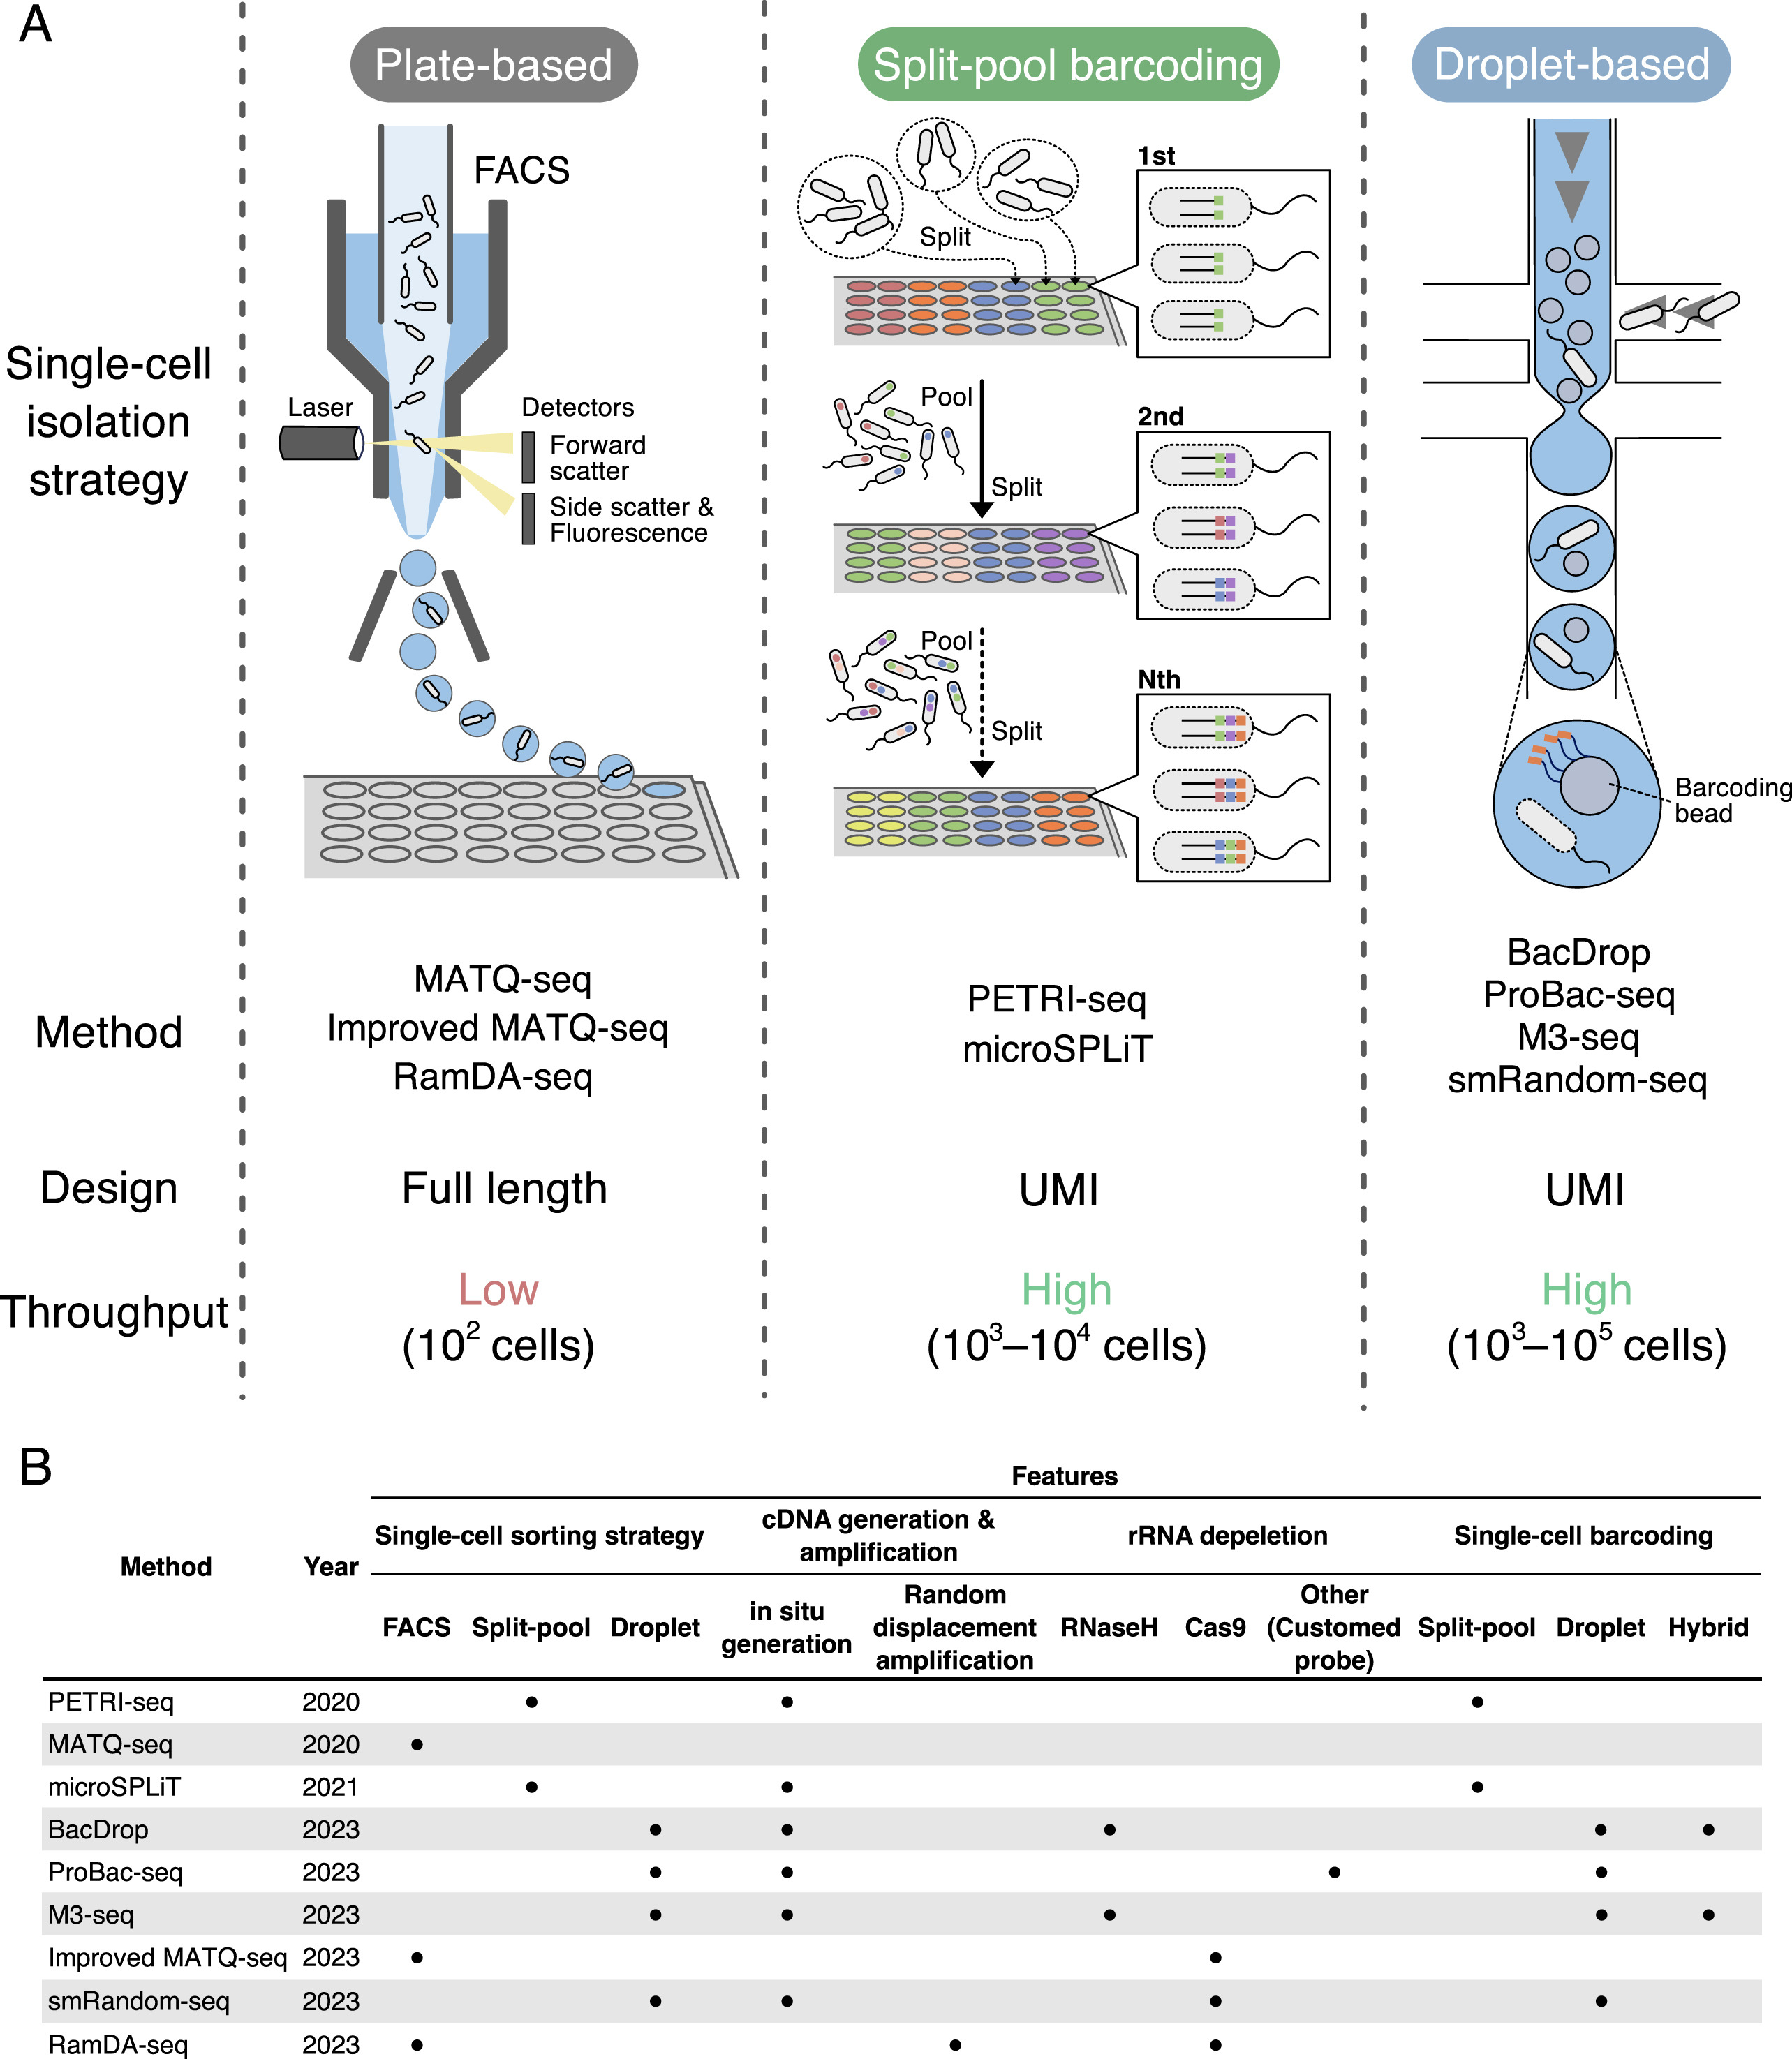
\includegraphics[keepaspectratio]{chapters/../figures/nishimura_review.jpg}}

}

\caption{\label{fig-nishimura_review}Overview of bacterial single-cell
RNA sequencing approaches. (A) Schematic summary of single-cell
isolation strategies employed in bacterial single-cell RNA-seq,
highlighting the key features and distinctions of each approach. FACS,
fluorescent activated cell sorting; UMI, unique molecular identifier.
(B) Summary of features of each bacterial single-cell RNA-seq method,
including MATQ-seq, RamDA-seq, PETRI-seq, microSPLiT, BacDrop,
ProBac-seq, M3-seq, and
smRandom-seq\textsuperscript{\citeproc{ref-nishimura2025}{22}}}

\end{figure}%

\section{MicroSPLiT sequencing library
preparation}\label{microsplit-sequencing-library-preparation}

\begin{figure}

\centering{

\pandocbounded{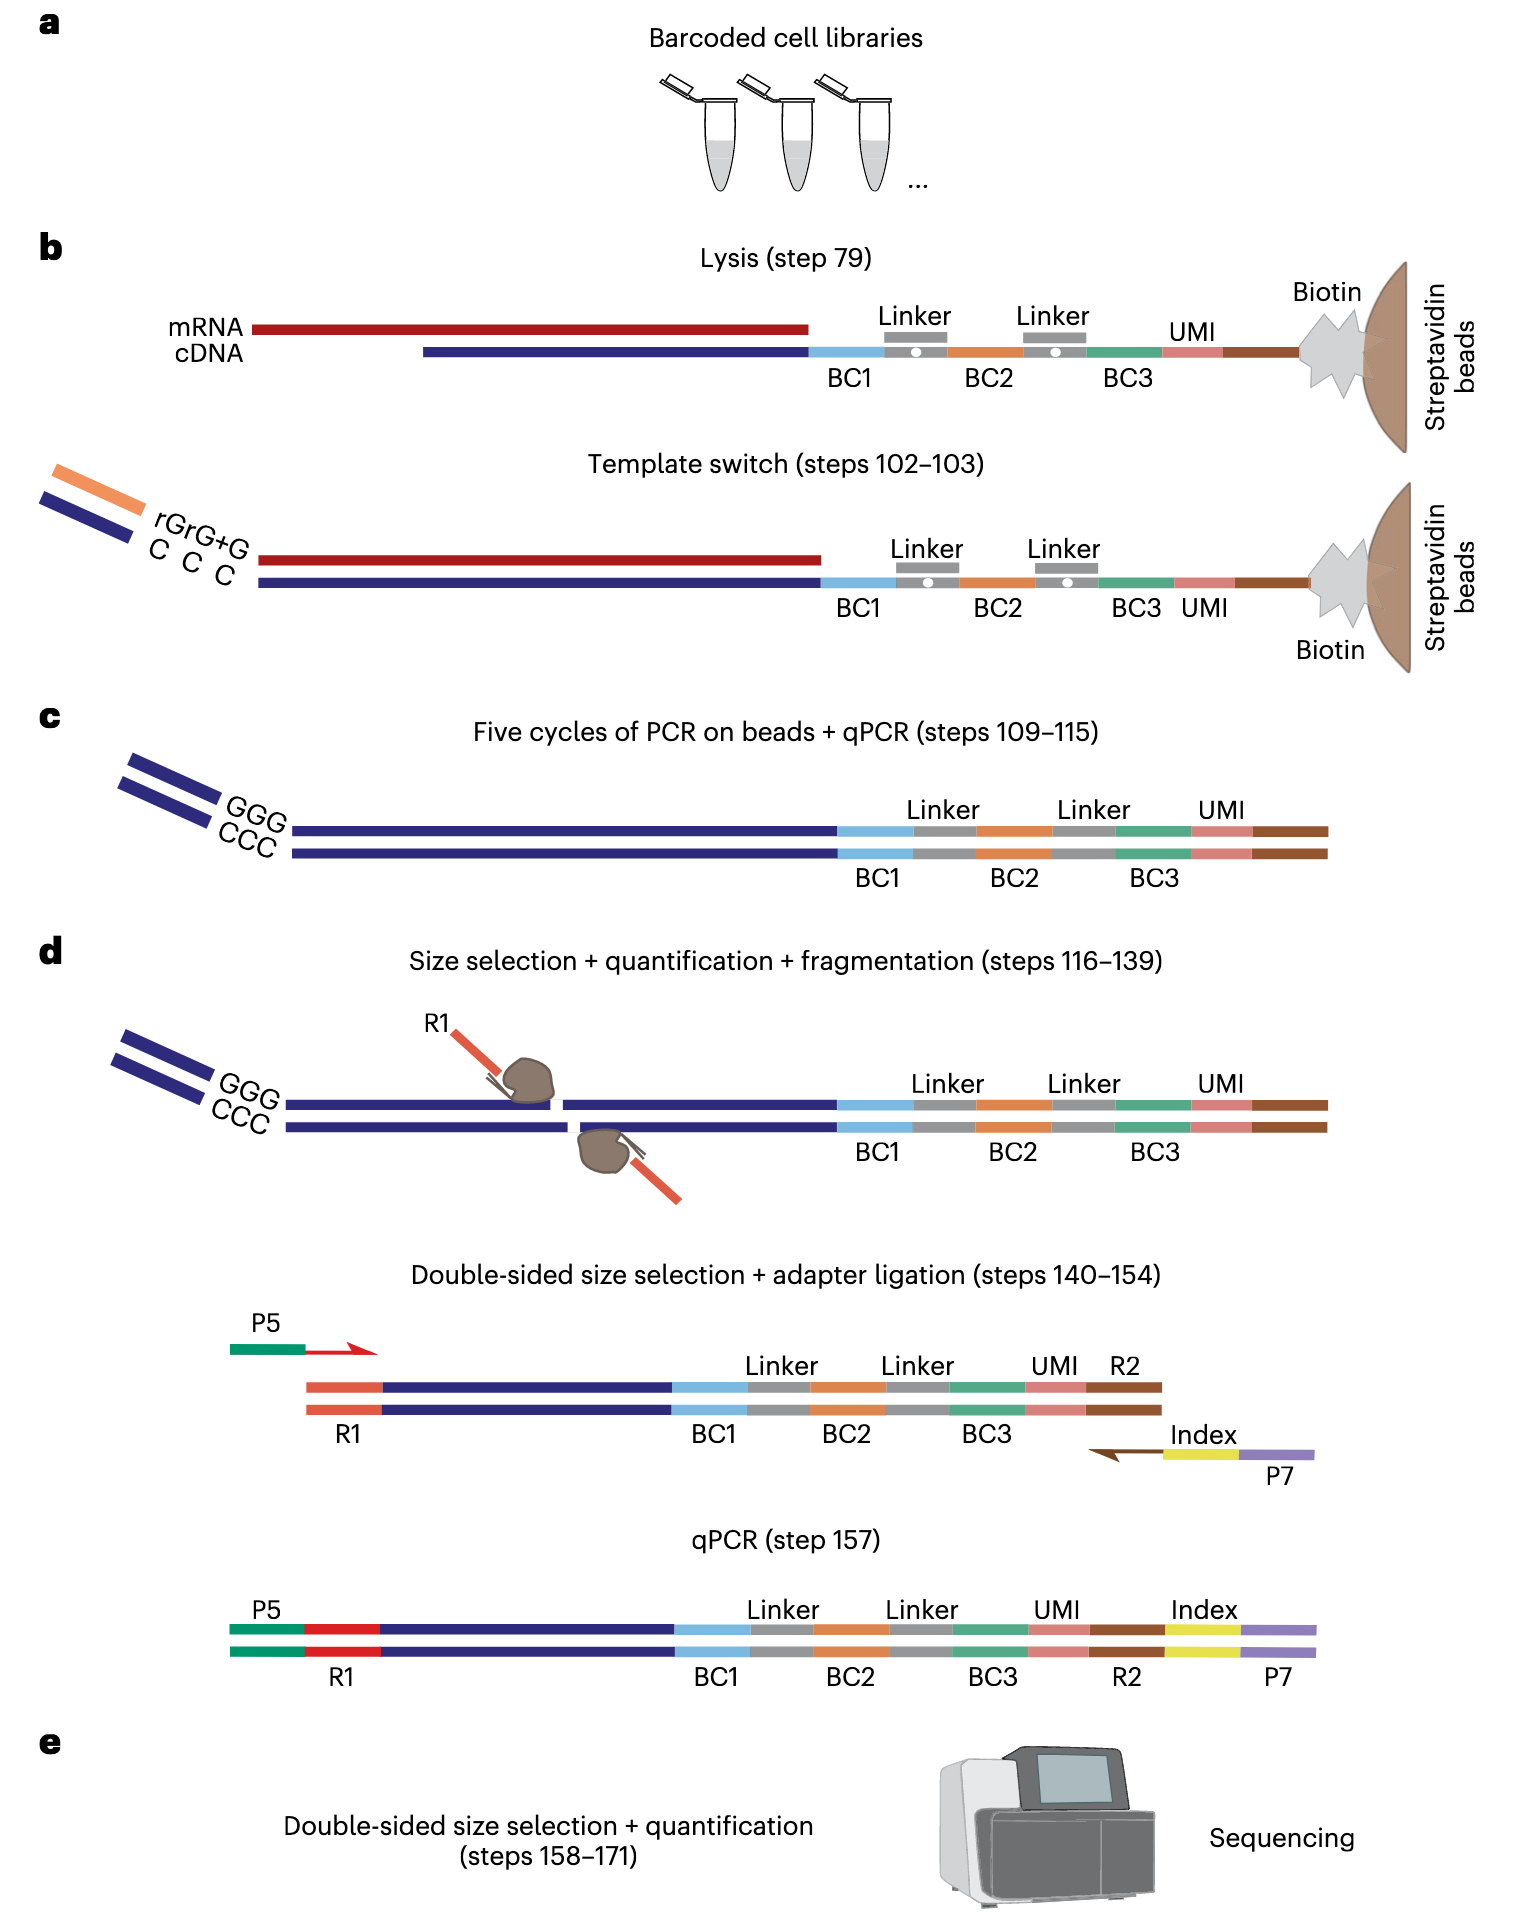
\includegraphics[keepaspectratio]{chapters/../figures/protocol_p2.png}}

}

\caption{\label{fig-protocol-p2}MicroSPLiT sequencing library
preparation. a, Selected sub-libraries with barcoded cells are lysed.
Because cDNA molecules primed with both random hexamer and poly-dT
primers undergo the same downstream reactions, only one of them is shown
for clarity. b, After lysis, cDNA is purified via streptavidin beads.
The cells then undergo an additional RT and template switching step. The
template switch primer has two RNA G bases and a locked nucleic acid G
base (`rGrG+G') sequence to facilitate the binding. c, cDNA is
amplified, and size is selected to eliminate the unwanted short product
(`dimer') from the cDNA amplification product. At this point, the size
and concentration of the cDNA product are quantified (Part 2, Step 127).
d, The library then undergoes fragmentation and adapter ligation. The
desired sequencing product containing the barcodes is amplified with the
primers for both the third barcode adapter and the ligation adapter,
which contain Read 1 (R1) and Read 2 (R2) sequences. Illumina P5 and P7
sequence adapters and a final sub-library index are also appended at
this final PCR step . e, A 0.5--0.7× double size selection then selects
out unwanted fragments. The final product's concentration and size are
measured before sequencing .}

\end{figure}%

\section{TSO removal statistics}\label{sec-appendix-tso}

The following table summarizes the number of R1 reads before and after
TSO removal for each sample, as well as the corresponding percentage.

\begin{longtable}[]{@{}llll@{}}
\caption{TSO removal statistics for each sample. The table shows the
total number of R1 reads, the number of R1 reads after TSO sequence
removal, and the corresponding
percentage.}\label{tbl-tso-removal}\tabularnewline
\toprule\noalign{}
Sample & Total R1 & R1 with TSO removed & Percentage (\%) \\
\midrule\noalign{}
\endfirsthead
\toprule\noalign{}
Sample & Total R1 & R1 with TSO removed & Percentage (\%) \\
\midrule\noalign{}
\endhead
\bottomrule\noalign{}
\endlastfoot
BC\_0076 & 631,393,326 & 153,472,373 & 24.3 \\
BC\_0077 & 325,495,590 & 90,142,002 & 27.7 \\
BC\_0079 & 379,108,253 & 102,386,519 & 27.0 \\
BC\_0080 & 397,654,767 & 99,430,515 & 25.0 \\
\end{longtable}

// Table added to summarize TSO removal efficiency for each sample. //
\ldots{} existing code \ldots{}

\section{Trimming pipeline steps}\label{sec-appendix-trimming-steps}

The following steps were performed sequentially for read trimming, as
implemented in the custom pipeline (see process\_sample.sh). Each step
is performed in paired-end mode to maintain synchronization between R1
and R2 files.

\begin{enumerate}
\def\labelenumi{\arabic{enumi}.}
\item
  \textbf{TSO trimming (Cutadapt):}\\
  Removal of template-switching oligo (TSO) sequences from R1 using
  Cutadapt. This step targets TSO sequences at the 5' end of cDNA reads
  to eliminate technical artifacts.

\begin{Shaded}
\begin{Highlighting}[]
\ExtensionTok{cutadapt} \AttributeTok{{-}j} \VariableTok{$\{SLURM\_CPUS\_PER\_TASK\}} \DataTypeTok{\textbackslash{}}
    \AttributeTok{{-}g} \StringTok{"AAGCAGTGGTATCAACGCAGAGTGAATGGG; min\_overlap=6; max\_errors=0.2"} \DataTypeTok{\textbackslash{}}
    \AttributeTok{{-}g} \StringTok{"CAGAGTGAATGGG; min\_overlap=6; max\_errors=0.2"} \DataTypeTok{\textbackslash{}}
    \AttributeTok{{-}{-}pair{-}filter}\OperatorTok{=}\NormalTok{both }\DataTypeTok{\textbackslash{}}
    \AttributeTok{{-}m}\NormalTok{ 20: }\DataTypeTok{\textbackslash{}}
    \AttributeTok{{-}{-}too{-}short{-}output} \StringTok{"}\VariableTok{$\{output\_dir\}}\StringTok{/}\VariableTok{$\{sample\_name\}}\StringTok{\_R1\_too\_short.fastq.gz"} \DataTypeTok{\textbackslash{}}
    \AttributeTok{{-}{-}too{-}short{-}paired{-}output} \StringTok{"}\VariableTok{$\{output\_dir\}}\StringTok{/}\VariableTok{$\{sample\_name\}}\StringTok{\_R2\_too\_short.fastq.gz"} \DataTypeTok{\textbackslash{}}
    \AttributeTok{{-}o} \StringTok{"}\VariableTok{$\{r1\_output\}}\StringTok{"} \DataTypeTok{\textbackslash{}}
    \AttributeTok{{-}p} \StringTok{"}\VariableTok{$\{r2\_output\}}\StringTok{"} \DataTypeTok{\textbackslash{}}
    \StringTok{"}\VariableTok{$\{r1\_input\}}\StringTok{"} \StringTok{"}\VariableTok{$\{r2\_input\}}\StringTok{"} \DataTypeTok{\textbackslash{}}
    \AttributeTok{{-}{-}report}\OperatorTok{=}\NormalTok{full }\DataTypeTok{\textbackslash{}}
    \AttributeTok{{-}{-}json} \StringTok{"}\VariableTok{$\{output\_dir\}}\StringTok{/}\VariableTok{$\{sample\_name\}}\StringTok{\_stats.json"}
\end{Highlighting}
\end{Shaded}
\item
  \textbf{Initial quality and adapter trimming (Fastp):}\\
  Removal of low-quality bases, polyG/polyX tails, and adapter sequences
  using Fastp. This step also removes the TruSeq Read 2 adapter and I7
  adapter at the end of R1 if present.

\begin{Shaded}
\begin{Highlighting}[]
\ExtensionTok{fastp} \DataTypeTok{\textbackslash{}}
    \AttributeTok{{-}i} \StringTok{"}\VariableTok{$\{r1\_input\}}\StringTok{"} \DataTypeTok{\textbackslash{}}
    \AttributeTok{{-}I} \StringTok{"}\VariableTok{$\{r2\_input\}}\StringTok{"} \DataTypeTok{\textbackslash{}}
    \AttributeTok{{-}o} \StringTok{"}\VariableTok{$\{r1\_output\}}\StringTok{"} \DataTypeTok{\textbackslash{}}
    \AttributeTok{{-}O} \StringTok{"}\VariableTok{$\{r2\_output\}}\StringTok{"} \DataTypeTok{\textbackslash{}}
    \AttributeTok{{-}{-}html} \StringTok{"}\VariableTok{$\{output\_dir\}}\StringTok{/}\VariableTok{$\{sample\_name\}}\StringTok{\_report.html"} \DataTypeTok{\textbackslash{}}
    \AttributeTok{{-}{-}json} \StringTok{"}\VariableTok{$\{output\_dir\}}\StringTok{/}\VariableTok{$\{sample\_name\}}\StringTok{\_report.json"} \DataTypeTok{\textbackslash{}}
    \AttributeTok{{-}{-}report\_title} \StringTok{"microSplit Initial Fastp Report {-} }\VariableTok{$\{sample\_name\}}\StringTok{"} \DataTypeTok{\textbackslash{}}
    \AttributeTok{{-}{-}compression}\NormalTok{ 4 }\DataTypeTok{\textbackslash{}}
    \AttributeTok{{-}{-}verbose} \DataTypeTok{\textbackslash{}}
    \AttributeTok{{-}{-}unpaired1} \StringTok{"}\VariableTok{$\{unpaired1\}}\StringTok{"} \DataTypeTok{\textbackslash{}}
    \AttributeTok{{-}{-}unpaired2} \StringTok{"}\VariableTok{$\{unpaired2\}}\StringTok{"} \DataTypeTok{\textbackslash{}}
    \AttributeTok{{-}{-}length\_required}\NormalTok{ 91 }\DataTypeTok{\textbackslash{}}
    \AttributeTok{{-}{-}dont\_overwrite} \DataTypeTok{\textbackslash{}}
    \AttributeTok{{-}{-}trim\_front1}\NormalTok{ 0 }\DataTypeTok{\textbackslash{}}
    \AttributeTok{{-}{-}trim\_front2}\NormalTok{ 0 }\DataTypeTok{\textbackslash{}}
    \AttributeTok{{-}{-}trim\_tail1}\NormalTok{ 0 }\DataTypeTok{\textbackslash{}}
    \AttributeTok{{-}{-}trim\_tail2}\NormalTok{ 0 }\DataTypeTok{\textbackslash{}}
    \AttributeTok{{-}{-}trim\_poly\_g} \DataTypeTok{\textbackslash{}}
    \AttributeTok{{-}{-}poly\_g\_min\_len}\NormalTok{ 10 }\DataTypeTok{\textbackslash{}}
    \AttributeTok{{-}{-}trim\_poly\_x} \DataTypeTok{\textbackslash{}}
    \AttributeTok{{-}{-}poly\_x\_min\_len}\NormalTok{ 12 }\DataTypeTok{\textbackslash{}}
    \AttributeTok{{-}{-}detect\_adapter\_for\_pe} \DataTypeTok{\textbackslash{}}
    \AttributeTok{{-}{-}adapter\_sequence}\OperatorTok{=}\NormalTok{ATCTCGTATGCCGTCTTCTGCTTGA }\DataTypeTok{\textbackslash{}}
    \AttributeTok{{-}{-}adapter\_sequence}\OperatorTok{=}\NormalTok{AGATCGGAAGAGCACACGTCTGAACTCCAGTCAC}
\end{Highlighting}
\end{Shaded}
\item
  \textbf{PolyA trimming (Cutadapt):}\\
  Removal of polyA stretches (\textgreater=12 nt) and all downstream
  sequences from R1 using Cutadapt, targeting polyA sequences introduced
  during library preparation. This step cleans reads with short cDNA
  that extend into the R2 complementary region, using polyA as a repeat
  sequence (read\_polyA from the library).

\begin{Shaded}
\begin{Highlighting}[]
\ExtensionTok{cutadapt} \AttributeTok{{-}j} \VariableTok{$\{SLURM\_CPUS\_PER\_TASK\}} \DataTypeTok{\textbackslash{}}
    \AttributeTok{{-}a} \StringTok{"A\{12\}; min\_overlap=12; max\_errors=0.2"} \DataTypeTok{\textbackslash{}}
    \AttributeTok{{-}{-}pair{-}filter}\OperatorTok{=}\NormalTok{both }\DataTypeTok{\textbackslash{}}
    \AttributeTok{{-}m}\NormalTok{ 20: }\DataTypeTok{\textbackslash{}}
    \AttributeTok{{-}{-}too{-}short{-}output} \StringTok{"}\VariableTok{$\{output\_dir\}}\StringTok{/}\VariableTok{$\{sample\_name\}}\StringTok{\_R1\_too\_short.fastq.gz"} \DataTypeTok{\textbackslash{}}
    \AttributeTok{{-}{-}too{-}short{-}paired{-}output} \StringTok{"}\VariableTok{$\{output\_dir\}}\StringTok{/}\VariableTok{$\{sample\_name\}}\StringTok{\_R2\_too\_short.fastq.gz"} \DataTypeTok{\textbackslash{}}
    \AttributeTok{{-}o} \StringTok{"}\VariableTok{$\{r1\_output\}}\StringTok{"} \DataTypeTok{\textbackslash{}}
    \AttributeTok{{-}p} \StringTok{"}\VariableTok{$\{r2\_output\}}\StringTok{"} \DataTypeTok{\textbackslash{}}
    \StringTok{"}\VariableTok{$\{r1\_input\}}\StringTok{"} \StringTok{"}\VariableTok{$\{r2\_input\}}\StringTok{"} \DataTypeTok{\textbackslash{}}
    \AttributeTok{{-}{-}report}\OperatorTok{=}\NormalTok{full }\DataTypeTok{\textbackslash{}}
    \AttributeTok{{-}{-}json} \StringTok{"}\VariableTok{$\{output\_dir\}}\StringTok{/}\VariableTok{$\{sample\_name\}}\StringTok{\_stats.json"}
\end{Highlighting}
\end{Shaded}

  This step trims polyA15 and longer stretches that may remain after the
  previous steps.
\item
  \textbf{Specific adapter trimming (Cutadapt):}\\
  Removal of the specific adapter sequence CCACAGTCTCAAGCAC from R1
  using Cutadapt (corresponds to the round 2 linker sequence). This step
  uses the round 2 linker barcode as a reference point and eliminates
  everything behind it, particularly useful for cleaning random hexamer
  sequences with short cDNA that extend into R2 complementary sequences.

\begin{Shaded}
\begin{Highlighting}[]
\ExtensionTok{cutadapt} \AttributeTok{{-}j} \VariableTok{$\{SLURM\_CPUS\_PER\_TASK\}} \DataTypeTok{\textbackslash{}}
    \AttributeTok{{-}a} \StringTok{"CCACAGTCTCAAGCAC; min\_overlap=6; max\_errors=0.1"} \DataTypeTok{\textbackslash{}}
    \AttributeTok{{-}{-}pair{-}filter}\OperatorTok{=}\NormalTok{both }\DataTypeTok{\textbackslash{}}
    \AttributeTok{{-}m}\NormalTok{ 20: }\DataTypeTok{\textbackslash{}}
    \AttributeTok{{-}{-}too{-}short{-}output} \StringTok{"}\VariableTok{$\{output\_dir\}}\StringTok{/}\VariableTok{$\{sample\_name\}}\StringTok{\_R1\_too\_short.fastq.gz"} \DataTypeTok{\textbackslash{}}
    \AttributeTok{{-}{-}too{-}short{-}paired{-}output} \StringTok{"}\VariableTok{$\{output\_dir\}}\StringTok{/}\VariableTok{$\{sample\_name\}}\StringTok{\_R2\_too\_short.fastq.gz"} \DataTypeTok{\textbackslash{}}
    \AttributeTok{{-}o} \StringTok{"}\VariableTok{$\{r1\_output\}}\StringTok{"} \DataTypeTok{\textbackslash{}}
    \AttributeTok{{-}p} \StringTok{"}\VariableTok{$\{r2\_output\}}\StringTok{"} \DataTypeTok{\textbackslash{}}
    \StringTok{"}\VariableTok{$\{r1\_input\}}\StringTok{"} \StringTok{"}\VariableTok{$\{r2\_input\}}\StringTok{"} \DataTypeTok{\textbackslash{}}
    \AttributeTok{{-}{-}report}\OperatorTok{=}\NormalTok{full }\DataTypeTok{\textbackslash{}}
    \AttributeTok{{-}{-}json} \StringTok{"}\VariableTok{$\{output\_dir\}}\StringTok{/}\VariableTok{$\{sample\_name\}}\StringTok{\_stats.json"}
\end{Highlighting}
\end{Shaded}
\item
  \textbf{Linker and additional adapter trimming (Cutadapt):}\\
  Removal of linker and additional adapter sequences from R1 using
  Cutadapt, to further clean the reads. This includes TruSeq Read 2
  adapter (AGATCGGAAGAGCACACGTCTGAACTCCAGTCA), Round 3 linker
  (AGTCGTACGCCGATGCGAAACATCGGCCAC), and Round 2 linker
  (CCACAGTCTCAAGCACGTGGAT).\\
  This step ensures that any remaining linker or adapter sequences are
  removed for certain libraries.

\begin{Shaded}
\begin{Highlighting}[]
\ExtensionTok{cutadapt} \AttributeTok{{-}j} \VariableTok{$\{SLURM\_CPUS\_PER\_TASK\}} \DataTypeTok{\textbackslash{}}
    \AttributeTok{{-}a} \StringTok{"CCACAGTCTCAAGCACGTGGAT; min\_overlap=6; max\_errors=0.2"} \DataTypeTok{\textbackslash{}}
    \AttributeTok{{-}a} \StringTok{"AGTCGTACGCCGATGCGAAACATCGGCCAC; min\_overlap=6; max\_errors=0.2"} \DataTypeTok{\textbackslash{}}
    \AttributeTok{{-}a} \StringTok{"AGATCGGAAGAGCACACGTCTGAACTCCAGTCA; min\_overlap=6; max\_errors=0.2"} \DataTypeTok{\textbackslash{}}
    \AttributeTok{{-}{-}pair{-}filter}\OperatorTok{=}\NormalTok{both }\DataTypeTok{\textbackslash{}}
    \AttributeTok{{-}m}\NormalTok{ 20: }\DataTypeTok{\textbackslash{}}
    \AttributeTok{{-}{-}too{-}short{-}output} \StringTok{"}\VariableTok{$\{output\_dir\}}\StringTok{/}\VariableTok{$\{sample\_name\}}\StringTok{\_R1\_too\_short.fastq.gz"} \DataTypeTok{\textbackslash{}}
    \AttributeTok{{-}{-}too{-}short{-}paired{-}output} \StringTok{"}\VariableTok{$\{output\_dir\}}\StringTok{/}\VariableTok{$\{sample\_name\}}\StringTok{\_R2\_too\_short.fastq.gz"} \DataTypeTok{\textbackslash{}}
    \AttributeTok{{-}o} \StringTok{"}\VariableTok{$\{r1\_output\}}\StringTok{"} \DataTypeTok{\textbackslash{}}
    \AttributeTok{{-}p} \StringTok{"}\VariableTok{$\{r2\_output\}}\StringTok{"} \DataTypeTok{\textbackslash{}}
    \StringTok{"}\VariableTok{$\{r1\_input\}}\StringTok{"} \StringTok{"}\VariableTok{$\{r2\_input\}}\StringTok{"} \DataTypeTok{\textbackslash{}}
    \AttributeTok{{-}{-}report}\OperatorTok{=}\NormalTok{full }\DataTypeTok{\textbackslash{}}
    \AttributeTok{{-}{-}json} \StringTok{"}\VariableTok{$\{output\_dir\}}\StringTok{/}\VariableTok{$\{sample\_name\}}\StringTok{\_stats.json"}
\end{Highlighting}
\end{Shaded}
\item
  \textbf{Final quality and length filtering (Fastp):}\\
  Final trimming with Fastp, including additional adapter removal,
  trimming of fixed bases from the 5' and 3' ends, and filtering for
  minimum read length to ensure high-quality output for downstream
  analysis.\\
  This step trims R1 at both 5' and 3' ends to keep only cDNA and ensure
  clean sequences for downstream analysis.

\begin{Shaded}
\begin{Highlighting}[]
\ExtensionTok{fastp} \DataTypeTok{\textbackslash{}}
    \AttributeTok{{-}i} \StringTok{"}\VariableTok{$\{r1\_input\}}\StringTok{"} \DataTypeTok{\textbackslash{}}
    \AttributeTok{{-}I} \StringTok{"}\VariableTok{$\{r2\_input\}}\StringTok{"} \DataTypeTok{\textbackslash{}}
    \AttributeTok{{-}o} \StringTok{"}\VariableTok{$\{r1\_output\}}\StringTok{"} \DataTypeTok{\textbackslash{}}
    \AttributeTok{{-}O} \StringTok{"}\VariableTok{$\{r2\_output\}}\StringTok{"} \DataTypeTok{\textbackslash{}}
    \AttributeTok{{-}{-}trim\_front1}\NormalTok{ 10 }\DataTypeTok{\textbackslash{}}
    \AttributeTok{{-}{-}trim\_front2}\NormalTok{ 0 }\DataTypeTok{\textbackslash{}}
    \AttributeTok{{-}{-}trim\_tail1}\NormalTok{ 16 }\DataTypeTok{\textbackslash{}}
    \AttributeTok{{-}{-}trim\_tail2}\NormalTok{ 0 }\DataTypeTok{\textbackslash{}}
    \AttributeTok{{-}{-}length\_required}\NormalTok{ 25 }\DataTypeTok{\textbackslash{}}
    \AttributeTok{{-}{-}detect\_adapter\_for\_pe} \DataTypeTok{\textbackslash{}}
    \AttributeTok{{-}{-}adapter\_sequence}\OperatorTok{=}\NormalTok{AAGCAGTGGTATCAACGCAGAGTGAATGGG }\DataTypeTok{\textbackslash{}}
    \AttributeTok{{-}{-}adapter\_sequence}\OperatorTok{=}\NormalTok{CCACAGTCTCAAGCACGTGGAT }\DataTypeTok{\textbackslash{}}
    \AttributeTok{{-}{-}adapter\_sequence}\OperatorTok{=}\NormalTok{AGTCGTACGCCGATGCGAAACATCGGCCAC }\DataTypeTok{\textbackslash{}}
    \AttributeTok{{-}{-}adapter\_sequence}\OperatorTok{=}\NormalTok{AGATCGGAAGAGCACACGTCTGAACTCCAGTCA }\DataTypeTok{\textbackslash{}}
    \AttributeTok{{-}{-}html} \StringTok{"}\VariableTok{$\{output\_dir\}}\StringTok{/}\VariableTok{$\{sample\_name\}}\StringTok{\_report.html"} \DataTypeTok{\textbackslash{}}
    \AttributeTok{{-}{-}json} \StringTok{"}\VariableTok{$\{output\_dir\}}\StringTok{/}\VariableTok{$\{sample\_name\}}\StringTok{\_report.json"} \DataTypeTok{\textbackslash{}}
    \AttributeTok{{-}{-}report\_title} \StringTok{"microSplit Final Fastp Report {-} }\VariableTok{$\{sample\_name\}}\StringTok{"} \DataTypeTok{\textbackslash{}}
    \AttributeTok{{-}{-}compression}\NormalTok{ 4 }\DataTypeTok{\textbackslash{}}
    \AttributeTok{{-}{-}verbose}
\end{Highlighting}
\end{Shaded}
\end{enumerate}

\section{Final effective command line of
STARsolo}\label{sec-appendix-starsolo}

\subsection{Computing Environment}\label{computing-environment}

The STARsolo analysis was performed on the GenOuest high-performance
computing cluster using the following specifications: - \textbf{Node
type}: bigmem (high-memory node) - \textbf{Memory allocation}: 500GB RAM
- \textbf{CPU threads}: 64 parallel threads

\subsection{STARsolo Command Line}\label{starsolo-command-line}

\begin{Shaded}
\begin{Highlighting}[]
\ExtensionTok{STAR} \DataTypeTok{\textbackslash{}}
\NormalTok{{-}{-}runThreadN 64 }\DataTypeTok{\textbackslash{}}
\NormalTok{{-}{-}genomeDir /path/to/genome\_index }\DataTypeTok{\textbackslash{}}
\NormalTok{{-}{-}readFilesIn }\DataTypeTok{\textbackslash{}}
\NormalTok{/path/to/input/merged\_trimmed{-}R1.fastq.gz }\DataTypeTok{\textbackslash{}}
\NormalTok{/path/to/input/merged\_trimmed{-}R2.fastq.gz }\DataTypeTok{\textbackslash{}}
\NormalTok{{-}{-}readFilesCommand gunzip }\AttributeTok{{-}c} \DataTypeTok{\textbackslash{}}
\NormalTok{{-}{-}outFileNamePrefix /path/to/output/starsolo\_output/ }\DataTypeTok{\textbackslash{}}
\NormalTok{{-}{-}outSAMtype BAM Unsorted }\DataTypeTok{\textbackslash{}}
\NormalTok{{-}{-}outFilterScoreMinOverLread 0 }\DataTypeTok{\textbackslash{}}
\NormalTok{{-}{-}outFilterMatchNmin 50 }\DataTypeTok{\textbackslash{}}
\NormalTok{{-}{-}outFilterMatchNminOverLread 0 }\DataTypeTok{\textbackslash{}}
\NormalTok{{-}{-}alignSJoverhangMin 1000 }\DataTypeTok{\textbackslash{}}
\NormalTok{{-}{-}alignSJDBoverhangMin 1000 }\DataTypeTok{\textbackslash{}}
\NormalTok{{-}{-}soloType CB\_UMI\_Complex }\DataTypeTok{\textbackslash{}}
\NormalTok{{-}{-}soloCBwhitelist }\DataTypeTok{\textbackslash{}}
\NormalTok{/path/to/barcodes/barcode\_round3.txt }\DataTypeTok{\textbackslash{}}
\NormalTok{/path/to/barcodes/barcode\_round2.txt }\DataTypeTok{\textbackslash{}}
\NormalTok{/path/to/barcodes/barcode\_round1.txt }\DataTypeTok{\textbackslash{}}
\NormalTok{{-}{-}soloFeatures Gene GeneFull }\DataTypeTok{\textbackslash{}}
\NormalTok{{-}{-}soloUMIdedup 1MM\_All }\DataTypeTok{\textbackslash{}}
\NormalTok{{-}{-}soloCBmatchWLtype 1MM }\DataTypeTok{\textbackslash{}}
\NormalTok{{-}{-}soloCBposition 0\_10\_0\_17 0\_48\_0\_55 0\_78\_0\_85 }\DataTypeTok{\textbackslash{}}
\NormalTok{{-}{-}soloUMIposition 0\_0\_0\_9 }\DataTypeTok{\textbackslash{}}
\NormalTok{{-}{-}soloMultiMappers Uniform}
\end{Highlighting}
\end{Shaded}

\subsection{STARsolo Parameters
Explanation}\label{starsolo-parameters-explanation}

This section details the key parameters used in our STARsolo analysis
and their significance:

\subsubsection{General STAR Parameters}\label{general-star-parameters}

\begin{itemize}
\tightlist
\item
  \texttt{-\/-runThreadN\ 64} : Use of 64 threads for parallel alignment
\item
  \texttt{-\/-genomeDir} : Path to the reference genome index
\item
  \texttt{-\/-readFilesIn} : Input FASTQ files (R1 and R2)
\item
  \texttt{-\/-readFilesCommand\ gunzip\ -c} : Command to decompress
  FASTQ.gz files
\item
  \texttt{-\/-outFileNamePrefix} : Prefix for output files
\item
  \texttt{-\/-outSAMtype\ BAM\ Unsorted} : Unsorted BAM output format
\end{itemize}

\subsubsection{Filtering Parameters}\label{filtering-parameters}

\begin{itemize}
\tightlist
\item
  \texttt{-\/-outFilterScoreMinOverLread\ 0} : Minimum filtering score
  relative to read length
\item
  \texttt{-\/-outFilterMatchNmin\ 50} : Minimum number of matching bases
  for a valid alignment
\item
  \texttt{-\/-outFilterMatchNminOverLread\ 0} : Minimum match ratio
  relative to read length
\item
  \texttt{-\/-alignSJoverhangMin\ 1000} and
  \texttt{-\/-alignSJDBoverhangMin\ 1000} : Maximum values for splice
  junction detection (set to maximum since bacterial genomes lack
  splicing)
\end{itemize}

\subsubsection{STARsolo-specific
Parameters}\label{starsolo-specific-parameters}

\begin{itemize}
\tightlist
\item
  \texttt{-\/-soloType\ CB\_UMI\_Complex} : Analysis type for cell
  barcodes (CB) and complex UMIs
\item
  \texttt{-\/-soloCBwhitelist} : List of valid cell barcodes for the
  three barcoding rounds
\item
  \texttt{-\/-soloFeatures\ Gene\ GeneFull} : Analysis of features at
  both gene and full transcript levels
\item
  \texttt{-\/-soloUMIdedup\ 1MM\_All} : UMI deduplication with one
  mutation tolerance
\item
  \texttt{-\/-soloCBmatchWLtype\ 1MM} : Cell barcode matching with one
  mutation tolerance
\item
  \texttt{-\/-soloCBposition} : Cell barcode positions in reads (3
  rounds)

  \begin{itemize}
  \tightlist
  \item
    Round 1: 0\_10\_0\_17
  \item
    Round 2: 0\_48\_0\_55
  \item
    Round 3: 0\_78\_0\_85
  \end{itemize}
\item
  \texttt{-\/-soloUMIposition\ 0\_0\_0\_9} : UMI position in reads
\item
  \texttt{-\/-soloMultiMappers\ Uniform} : Uniform distribution of
  multi-mapped reads
\end{itemize}

These parameters were chosen to optimize single-cell detection while
maintaining high alignment quality and accounting for the complexity of
our three-round barcoding protocol.

Each step is performed in paired-end mode to ensure synchronization
between R1 and R2 files. See the pipeline script for implementation
details.

\begin{itemize}
\tightlist
\item
  plan de plaque
\item
  librairies avec TSO
\item
  tableau choix de profondeur / nombre de cellules
\item
  mettre difference entre experience de kuhina et la notre pour les
  resultats de Starsolo
\end{itemize}

\chapter{Annexe B: erferfrefref}\label{annexe-b}

\section{summary stats and features.stats for
Gene}\label{summary-stats-and-features.stats-for-gene}

\begin{verbatim}
                                     nUnmapped      114628761
                                    nNoFeature       20579292
                                 nAmbigFeature      934096737
                         nAmbigFeatureMultimap      934096737
                                      nTooMany              0
                                 nNoExactMatch         124864
                                   nExactMatch     4458742628
                                        nMatch      964094047
                                  nMatchUnique       30022209
                                 nCellBarcodes         689818
                                         nUMIs       29709734
\end{verbatim}

Number of Reads,1284475633 Reads With Valid Barcodes,0.85576 Sequencing
Saturation,0.0104081 Q30 Bases in CB+UMI,0.955089 Q30 Bases in RNA
read,0.957923 Reads Mapped to Genome: Unique+Multiple,0.895694 Reads
Mapped to Genome: Unique,0.0363836 Reads Mapped to Gene: Unique+Multipe
Gene,0.750574 Reads Mapped to Gene: Unique Gene,0.0233731 Estimated
Number of Cells,27268 Unique Reads in Cells Mapped to Gene,11121465
Fraction of Unique Reads in Cells,0.370441 Mean Reads per Cell,407
Median Reads per Cell,331 UMIs in Cells,10998607 Mean UMI per Cell,403
Median UMI per Cell,327 Mean Gene per Cell,253 Median Gene per Cell,221
Total Gene Detected,5894

\section{warning}\label{warning-2}

!!!!! WARNING: while processing
sjdbGTFfile=/projects/microsplit/data/processed\_data/STARsolo\_result/merged\_trimmed/merged/raw\_data/genome\_annotation/genome\_annotation\_PsR401\_fixed.gtf,
line: CP125962.1 Genbank exon 298557 300953 . - 0 transcript\_id
``gene-QLH64\_29550''; gene\_id ``gene-QLH64\_29550''; gene\_name
``QLH64\_29550''; exon end = 300953 is larger than the chromosome
CP125962.1 length = 299955 , will skip this exon

Log of the STARsolo run : Alignment statistics: -----------------------
Number of input reads \textbar{} 1284475633 Average input read length
\textbar{} 135 Uniquely mapped reads number \textbar{} 46733841 Uniquely
mapped reads \% \textbar{} 3.64\% Number of reads mapped to multiple
loci \textbar{} 1103762730 \% of reads mapped to multiple loci
\textbar{} 85.93\% Number of reads unmapped: other \textbar{} 128049614
\% of reads unmapped: other \textbar{} 9.97\% Mismatch rate per base, \%
\textbar{} 0.38\% Fri May 30 15:39:42 CEST 2025 - Pipeline completed!

\subsection{Pretest STARSolo on BC\_0077 without trimming
:}\label{pretest-starsolo-on-bc_0077-without-trimming}

\begin{verbatim}
                                    nNoAdapter              0
                                        nNoUMI              0
                                         nNoCB              0
                                        nNinCB              0
                                       nNinUMI        4467771
                               nUMIhomopolymer        4325324
                                      nTooMany              0
                                      nNoMatch       66837523
                           nMismatchesInMultCB        1680783
                                   nExactMatch      234544811
                                nMismatchOneWL       13639378
                             nMismatchToMultWL              0
\end{verbatim}

barcodes stats

\subsubsection{Genfull summary stats}\label{genfull-summary-stats}

\begin{longtable}[]{@{}ll@{}}
\toprule\noalign{}
Metric & Count \\
\midrule\noalign{}
\endhead
\bottomrule\noalign{}
\endlastfoot
nUnmapped & 89,425,075 \\
nNoFeature & 1,000,851 \\
nAmbigFeature & 152,909,678 \\
nAmbigFeatureMultimap & 152,443,034 \\
nTooMany & 0 \\
nNoExactMatch & 185,805 \\
nExactMatch & 729,180,878 \\
nMatch & 157,719,964 \\
nMatchUnique & 4,847,425 \\
nCellBarcodes & 168,346 \\
nUMIs & 305,287 \\
\end{longtable}

\begin{longtable}[]{@{}ll@{}}
\toprule\noalign{}
Metric & Value \\
\midrule\noalign{}
\endhead
\bottomrule\noalign{}
\endlastfoot
Number of Reads & 325,495,590 \\
Reads With Valid Barcodes & 76.19\% \\
Sequencing Saturation & 93.70\% \\
Q30 Bases in CB+UMI & 92.28\% \\
Q30 Bases in RNA read & 86.19\% \\
Reads Mapped to Genome: Unique+Multiple & 58.16\% \\
Reads Mapped to Genome: Unique & 2.15\% \\
Reads Mapped to GeneFull: Unique+Multiple & 48.46\% \\
Reads Mapped to GeneFull: Unique & 1.49\% \\
Estimated Number of Cells & 66,026 \\
Unique Reads in Cells Mapped to GeneFull & 3,538,648 \\
Fraction of Unique Reads in Cells & 73.00\% \\
Mean Reads per Cell & 53 \\
Median Reads per Cell & 36 \\
UMIs in Cells & 202,967 \\
Mean UMI per Cell & 3 \\
Median UMI per Cell & 2 \\
Mean GeneFull per Cell & 2 \\
Median GeneFull per Cell & 2 \\
Total GeneFull Detected & 5,295 \\
\end{longtable}

\subsubsection{Gene summary stats}\label{gene-summary-stats}

\begin{verbatim}
                                     nUnmapped       89425075
                                    nNoFeature        7350074
                                 nAmbigFeature      147588031
                         nAmbigFeatureMultimap      147588029
                                      nTooMany              0
                                 nNoExactMatch         182600
                                   nExactMatch      704353731
                                        nMatch      151371640
                                  nMatchUnique        3820029
                                 nCellBarcodes         135433
                                         nUMIs         224743
\end{verbatim}

Number of Reads,325495590 Reads With Valid Barcodes,0.76192 Sequencing
Saturation,0.941167 Q30 Bases in CB+UMI,0.922758 Q30 Bases in RNA
read,0.861863 Reads Mapped to Genome: Unique+Multiple,0.581583 Reads
Mapped to Genome: Unique,0.0215405 Reads Mapped to Gene: Unique+Multipe
Gene,0.46505 Reads Mapped to Gene: Unique Gene,0.011736 Estimated Number
of Cells,47264 Unique Reads in Cells Mapped to Gene,2582244 Fraction of
Unique Reads in Cells,0.675975 Mean Reads per Cell,54 Median Reads per
Cell,40 UMIs in Cells,136574 Mean UMI per Cell,2 Median UMI per Cell,2
Mean Gene per Cell,2 Median Gene per Cell,2 Total Gene Detected,4838

\chapter{Annexe C: codcefe}\label{annexe-c}

\clearpage
\thispagestyle{empty}
\vspace*{\fill}
\vspace*{\fill}
\clearpage



% Back cover content
\newpage  % Force a new page
\thispagestyle{empty}  % Page without header or footer
\begin{center}
  {\Huge \textbf{Master's Thesis in Bioinformatics}} \\[2cm]
  {\Large \textbf{University of Rennes}} \\[1cm]
  
\includegraphics[width=0.4\textwidth]{figures/rapport/logo_Univ_Rennes.png} \\[1cm]
  
\includegraphics[width=0.6\textwidth]{figures/rapport/couverture.png} \\[1cm]
  \begin{minipage}{0.8\textwidth}
    \centering
    \textit{This thesis was conducted in the framework of the Master's program in Bioinformatics at the University of Rennes. The research presented here contributes to the field of computational biology and bioinformatics.}
  \end{minipage} \\[1cm]
  \begin{minipage}{0.8\textwidth}
    \centering
    \small
    \textit{© Valentin Goupille - ?meta:year \\ All rights reserved}
  \end{minipage}
\end{center} 


\end{document}
